\documentclass{ucbthesis}

% Double spacing, if you want it.
% \def\dsp{\def\baselinestretch{2.0}\large\normalsize}
% \dsp

% If the Grad. Division insists that the first paragraph of a section
% be indented (like the others), then include this line:
% \usepackage{indentfirst}


% For revision control
\usepackage{rcs-multi}
\rcsid{$Id$}
\rcsid{$Header$}
\rcskwsave{$Author$}
\rcskwsave{$Date$} 
\rcskwsave{$Revision$}
%\rcsRegisterAuthor{devangel}{Dennis Jos{\'e} Evangelista}
\rcsRegisterAuthor{devangel}{Dennis J. Evangelista}

% I typically use these
\usepackage{graphicx}
\usepackage[usenames,dvipsnames]{color}
\usepackage{makeidx}
\usepackage{siunitx}
\usepackage{rotating}
\usepackage{multirow}
\usepackage{colortbl}


% PDF metadata
\usepackage{url}
\usepackage{hyperref}
\hypersetup{pdftitle={Something about Aerial Righting, Directed Aerial Descent, Maneuverability and Stability, and their Implications for the Evolution of Flight in Vertebrates}}
%\hypersetup{pdfauthor={Dennis Jos{\'e} Evangelista}}
\hypersetup{pdfauthor={Dennis J. Evangelista}}
\hypersetup{pdfsubject={biomechanics}}
\hypersetup{pdfkeywords={biomechanics, evolution, integrative biology, organismic}}
\hypersetup{colorlinks=true,citecolor=Violet,linkcolor=Blue,urlcolor=Red}
\hypersetup{bookmarks=true,bookmarksopen=true,hyperfootnotes=false,pdfpagemode=UseOutlines}

% Biology style references
\usepackage[round, sort&compress]{natbib}
\setcitestyle{authoryear, round, comma, aysep={;}, yysep={,}, notesep={, }}
\bibliographystyle{abbrvnat}
%\def\newblock{\hskip .11em plus .33em minus .07em} % bug workaround
% show doi in citations
\newcommand*{\doi}[1]{\href{http://dx.doi.org/\detokenize{#1}}{\texttt{doi:\detokenize{#1}}}}
\renewcommand\bibname{References}
\usepackage{bibentry}


% For chapter bibliographies
%\usepackage[sectionbib,duplicate]{chapterbib}

% For chapter abstracts
%\newenvironment{chabstract}{\begin{quote}\small}{\end{quote}}
%\newenvironment{chabstract}{\section*{}}{}

% Set section depth on table of contents
\setcounter{secnumdepth}{3}

% Use AMS math
\usepackage{amsmath}

% Yonatan used these?
%\usepackage{setspace}
%\usepackage{lscape}
%\usepackage{lineno}   % line numbering
%\modulolinenumbers[5] % line numbering
%\usepackage[hang,small,bf]{caption} % captions?
%\usepackage{xspace}

% Commands for Genus species names
\newcommand{\species}[1]{\emph{#1}}
\newcommand{\Calypteanna}{\species{Calypte anna}}
\newcommand{\Draco}{\species{Draco}}
\newcommand{\Archaeopteryx}{\species{\dag Archaeopteryx}}
\newcommand{\Microraptor}{\species{\dag Microraptor}}
\newcommand{\Microraptorgui}{\species{\dag Microraptor gui}}
\newcommand{\Anchiornis}{\species{\dag Anchiornis}}
\newcommand{\Mgui}{\species{\dag M.\ gui}}
\newcommand{\Drosophila}{\species{Drosophila}}
\newcommand{\Alectorischukar}{\species{Alectoris chukar}}
\newcommand{\Achukar}{\species{A.\ chukar}}
\newcommand{\Alectoris}{\species{Alectoris}}
\newcommand{\Anasplatyrhynchos}{\species{Anas platyrhynchos}}
\newcommand{\Aplatyrhynchos}{\species{A.\ platyrhynchos}}
\newcommand{\Anas}{\species{Anas}}
\newcommand{\Rhamphorynchus}{\species{\dag Rhamphorynchus}}
\newcommand{\Pteranodon}{\species{\dag Pteranodon}}
\newcommand{\Pterodactylus}{\species{\dag Pterodactylys}}
\newcommand{\Onychonycteris}{\species{\dag Onychonycteris}}
\newcommand{\Pteropus}{\species{Pteropus}}
\newcommand{\sixDOF}{six degree-of-freedom}
\newcommand{\Larus}{\species{Larus}}
\newcommand{\Oncorhynchus}{\species{Oncorhynchus}}
\newcommand{\Chaetodon}{\species{Chaetodon}}
\newcommand{\Hippocampus}{\species{Hippocampus}}
\newcommand{\vonKarman}{von K\'{a}rman}
\DeclareMathOperator*{\argmin}{\arg\!\min}







% Declarations for Front Matter
\title{Aerial righting, directed aerial descent, and maneuvering in the evolution of flight in birds}
%\title{Something about Aerial Righting, Directed Aerial Descent, Maneuverability and Stability, and their Implications for the Evolution of Flight in Vertebrates}
\author{Dennis J.\ Evangelista}
\degreesemester{Fall}
\degreeyear{2012}
\degree{Doctor of Philosophy}
\chair{Professor Robert Dudley}
\othermembers{Professor J.\ A.\ McGuire \\
  Professor Ronald Fearing}
\numberofmembers{3}
\prevdegrees{B.S., Mechanical Engineering (Massachusetts Institute of Technology) 1999\\
B.S., Electrical Engineering (Massachusetts Institute of Technology) 1999\\
M.Eng., Electrical Engineering and Computer Science (Massachusetts Institute of Technology) 1999\\
M.S.E.S., Mechanical Engineering (Naval Postgraduate School) 2001}
\field{Integrative Biology}
\campus{Berkeley}

\makeindex



% if only working on one chapter for the day
%\includeonly{ch-1,app-cam,app-tdd,app-ang}

\begin{document}
\maketitle
\approvalpage
\copyrightpage
% (This is included by thesis.tex; you do not latex it by itself.)

\begin{abstract}
% The text of the abstract goes here.  If you need to use a \section
% command you will need to use \section*, \subsection*, etc. so that
% you don't get any numbering.  You probably won't be using any of
% these commands in the abstract anyway.
Look at aerial righting and directed aerial descent in Chukar partridges.  In parallel, look at aerodynamic implications of different theropod and bird morphologies.  Consider some the effect of body size on damage and the effect of size and shape on turbulent noise pickup from turbulent flows.  Possibly to wrap up, weave all of these together in a phylogenetic framework. 
\end{abstract}


\frontmatter
\begin{dedication}
\null\vfil
\begin{center}
Dedication here
\end{center}
\vfil\null
\end{dedication}

\tableofcontents\clearpage
\listoffigures\clearpage
\listoftables
\begin{acknowledgements}
I want to thank my advisor for advising me.
\end{acknowledgements}


\mainmatter %\pagestyle{headings}
\chapter{Introduction}

\rcsid{$Id$}
\rcsid{$Header$}
\rcskwsave{$Author$}
\rcskwsave{$Date$} 
\rcskwsave{$Revision$}


%\begin{abstract}
This introductory chapter provides a roadmap for the thesis.  The over-arching question is what is the role of aerial righting, directed aerial descent, and maneuvering in general in the early evolution of flight in birds.  To address this question, three main studies are conducted:  a study of incipient flight behaviors in young birds over ontogeny; a detailed study of maneuvering using physical models of a likely ancestral bird morphology; and a comparative study of maneuvering ability examining several stem-group birds.  In addition to these, several side examinations necessary for benchmarking methods were serendipitously used to comment on broader questions of maneuvering ability within the vertebrates.  
%\end{abstract}

\section*{Introduction}
Flight among vertebrates is widespread.  Flight can be quite advantageous to fliers, enabling rapid or long distance travel and access to new resources.  Clades that fly are able to disperse and colonize, possibly enhancing diversification (citation?).  While historically, some may have considered ``powered'' flight restricted to birds, bats, and pterosaurs, \citet{Dudley:2011}, citing \citep{Rayner:1988, Norberg:1990} noted that gliding using obvious aerodynamic structures has evolved independently at least 30 times in mammals, reptiles, and amphibians.  Furthermore, aerial behaviors can occur in the absence of obvious aerodynamic surfaces, such as in directed aerial descent in canopy ants \citep{Yanoviak:2005, Yanoviak:2011} and bristletails \citep{Yanoviak:2008}.  Previous literature includes many well established, yet arbitrary definition of terms such as ``powered'' flight, parachuting, and gliding, all of which have muddied the comparative picture.  When one considers that all of these aerial behaviors require production and control of forces and moments in the air, it becomes clear that these are all a continuum of behaviors which vary primarily in the magnitude of the forces produced \citep{Dudley:2011}.  This shift in perspective suggests a generalized biomechanical scenario (maneuvering hypothesis) for the acquisition of aerial behaviors \citep{Dudley:2011}, shown in Table~\ref{tbl:scenario}.   
\begin{table}
\caption{Generalized biomechanical scenario for the acquisition of aerial behaviors and flight, repeated from \citep{Dudley:2011}}
\label{tbl:scenario}
\begin{center}
\begin{tabular}{l}
1. Arboreality; residence on elevated substrate \\
2. Jumping (either volitional or via startle reflex); falling \\
3. Aerial righting and landing reflexes \\
4. Parachuting (drag based descent) \\
5. Directed aerial descent (lift-based and drag-based; steep glide angles) \\
6. Gliding (predominantly lift-based; shallow glide angles) \\
7. Elaboration of wings and maneuvers \\
8. Flapping flight \\
\end{tabular}
\end{center}
\end{table}

Flight is constrained by physics and aerodynamics, which are invariant to ancestry and historical accident.  The maneuvering hypothesis predicts that 1) incipient maneuvering ability will be observed early on in the development of flight, both within an individual and within a clade; and 2) mechanisms of maneuvering, which are physically constrained, should show patterns of convergence among many taxa. In contrast, (some people would predict something different) (citations).  (explain Padian, Dial and WAIR).  A complete test of the maneuvering hypothesis requires a broad sampling of the taxa that engage in aerial behavior, and these are indeed underway (within vertebrates, Byrnes, Socha, Zhuang, Jusufi; within invertebrates, Munk, Zeng).
     
This thesis will further test maneuvering hypotheses of the evolution of flight, specifically by testing for incipient maneuvering ability in young birds during ontogeny (Chapter~\ref{sec:Chukar}), and by examining maneuvering ability in birds and their theropod ancestors (Chapters~\ref{sec:Microraptor} and \ref{sec:Comparative}).  Chapter~\ref{sec:Chukar} provides the first systematic exploration of aerial righting and directed aerial descent in birds, including shifts in function that correspond with the transitional stages identified in \citep{Dudley:2011}.  Chapter~\ref{sec:Microraptor} examines the functional consequences of early bird forms for maneuvering, and how function shifts with glide angle.  These are then examined in a phylogenetic and historical context in Chapter~\ref{sec:Comparative}.  The results provide multiple lines of evidence in support of the scenario of \citep{Dudley:2011}.  Furthermore, the two-pronged approach is expected to be robust against the shortcomings of either approach individually:  confounding ontogeny with evolution (as may be the case in \citep{Dial:2003}); or inferring implausible functions from paleontological material in the absence of proper benchmarking against live animals (need example of this? Padian?).

A schedule for completion is attached at the end of this document as Figure~\ref{fig:sched}.

%To further address aerodynamic hypotheses of the evolution of flight stemming from maneuvering, I would like to develop physical and computational models capable of describing the control effects of body movements considering two main phenomena: aerodynamic forces and inertial reactions.  First I will develop quasi-steady models to address steady aerodynamic forces using model tests and live animal data collected by others.  Second, I will use live animal data to extend these models for forces generated by inertia and aerodynamics during flapping and whipping of appendages.  Third, I will consider how noise gets injected into the models from the environment using additional physical and computational models.  The models will allow me to revisit the phylogenies of several flying animals to examine how what I have seen maps onto them, directly addressing previous criticism of aerodynamic hypotheses as wishful paradigms not in evidence.  

%\citep{Dial:2003, Dial:2008}.

\section{Biomechanics of the aerial righting response and directed aerial descent during ontogeny in young birds}
\label{sec:Chukar}
An aerial righting response allows falling animals to reorient the body dorsoventrally, presumably to initiate gliding/parachuting and subsequent landing without injury.  As fliers must fly in unpredictable environments, subject to disturbances from wind gusts, navigational hazards, predators, or widely spread desirable resources, an animal in the air may need to further direct its descent by maneuvering.

The focal species for this chapter is the Chukar Partridge (\Alectorischukar), a ground-dwelling game bird native to Asia introduced to the United States.  \Achukar\ was also the model system in studies of wing-assisted incline running (WAIR) \citep{Dial:2003, Dial:2008}; this allows comparison of our results with existing data purportedly in support of an alternate hypothesis.  Abbreviated comparisons were conducted with Chickens (\emph{Gallus gallus}) as a pilot study; and are to be conducted with Ducks (\emph{Anas platyrhynchos}; also \emph{Aix sp.}) in order to examine aerial righting and directed aerial descent in a species with a slower developmental trajectory, endpoint of long distance migratory flight, and ecologically-relevant use of directed aerial descent early in ontogeny (tree nesting in Wood Ducks).

%Alternative study organisms could include chickens or ducks (readily available from agricultural sources and able to be re-homed following experiments) or other birds in families that have evolved flightlessness (Ratites, penguins, kakapo parrots) or compromised flight abilities (various other running galliforms, puffins, cormorants).  However, unfortunately, unlike in stick insects, none of these has reversed the wing loss.  Another possibility is those birds for whom directed aerial descent in chicks is ecologically relevant (tree-nesting birds like murrelets or wood ducks).

\subsection{Aerial righting in Chukar Partridges (\Alectorischukar)}
Chukar Partridge chicks were hatched from eggs and subjected to drop tests from 1 day post hatching (dph) through 30 dph.  Aerial righting was observed through use of \SI{500}{frame\per\second} high speed video and \SI{60}{frame\per\second} high definition (HD) video to obtain detailed kinematics and trajectories.  Initially, at \SI{1}{dph}, chicks do little to alter their fall compared to a falling passive projectile.  By \SI{4}{dph}, birds exhibit righting by rolling using asymmetric flapping, in which one wing is strongly flapped while the other wing is flapped weakly or not flapped at all.  At \SI{10}{dph}, chicks begin transitioning to righting in pitch, using symmetric flapping with protracted wings.  By \SI{14}{dph}, chicks are able to slow their descent and exhibit clear modification of their trajectory to head towards targets of interest; strong directed aerial descent ability becomes apparent shortly after. Manipulations were also carried out during the experiment to show that righting is not visually mediated and that righting requires use of the wings. 

Experiments and data collection for this experiment are complete as of September 2011; detailed analysis is currently underway and should be complete by December.  Analysis will include success (\%) righting, body orientation, max acceleration or terminal velocity, rate of change of orientation, wingbeat frequency, etc. as well as morphometrics and body mass as a function of age. A series of repeated measures analyses of variance are planned to examine individual effects. Observed kinematics will also be compared to simple models (heave, roll) of falling birds.  

\subsection{Directed aerial descent in Chukar Partridges (\Alectorischukar)}
Directed aerial descent is studied using the same techniques as for aerial righting.  Chukar Partridge chicks were hatched and subjected to drop tests, which were filmed with \SI{500}{frame\per\second} high speed video and multiple \SI{60}{frame\per\second} HD video.  Trajectories are obtained using 3D camera calibration; they are then compared to a null model of a passive projectile to detect onset of directed aerial descent.  After onset of directed aerial descent, flight abilities are examined from maximal trajectories over ontogeny.  Preliminary results show the techniques used to maneuver do not change much during subsequent development from directed aerial descent to full flight ability.  Manipulations were attempted to augment tail inertia; manipulations were also carried out to trim wings and to check that directed aerial descent is visually mediated.

Experiments and data collection for this experiment are complete as of September 2011; detailed analysis is currently underway and should be complete by December.  The detailed analysis will include 3D trajectory reconstruction and tests comparing trajectories to a passive projectile null model to identify onset of directed descent.  Inertia manipulations were not successful but this may be addressed in analysis using suitably chosen computational models \citep{Jusufi:2008}.  As part of the analysis, computational models based on detailed kinematics may also be used to examine reachability and controllability of pitch and roll modes using movements of the wings, legs, etc. 

\subsection{Comparison between \Achukar\ and slower-developing migratory ducks}
Starting in October 2011, an abbreviated comparison will be conducted with Ducks (\emph{Anas platyrhynchos}; also \emph{Aix sp.}) in order to examine timing and pattern in a species with a slower developmental trajectory, endpoint of long distance migratory flight, and ecologically-relevant use of directed aerial descent early in ontogeny (tree nesting in \emph{Aix}).  The expectation / prediction from maneuvering hypotheses is all the same stages will occur; that aerial righting will occur early; strong directed aerial descent will not occur until wing feathers open, with the possibility of weak yawing or rolling earlier, using inertial mechanisms.  The experiments are planned to be conducted between October and November 2011, with completion in early Spring 2012. 

%
%Among vertebrates, aerial righting is likely widespread \citep{Dudley:2007}.  Aerial righting can be achieved in cats and humans using zero-angular-momentum turns in which the body is twisted in sequence to rotate without external aerodynamic torque \citep{Kane:1969, Frohlich:1970, Liu:1985, Edwards:1986}.  In house geckos, aerial righting is similarly accomplished using torques generated by rapid rotation and nutation of the tail \citep{Jusufi:2008}.  Among terrestrial arthropods, aerial righting is currently under study in ants (Munk, in preparation) and stick insects (Zeng, in preparation), and preliminary work indicates aerodynamic torques dominates aerial righting (compared to inertial torques) in smaller life stages.    
%
%(Has aerial righting been described in extant archosaurs, and have previous aerial righting studies considered size and aerodynamic effects?)  Do young birds possess an aerial righting reflex?  If so, how is aerial righting accomplished, and how does it change during ontogeny? 
%
%The models developed in part 1 are OK for quasi-static conditions, but they need to be extended for flapping of wings or true whipping of tails. 
%
%From \citet{Jusufi:2008} we know that tail inertia is able to produce turns and movements in falling geckoes.  Similar studies are currently underway in \emph{Scleropus} lizards (Talia Moore) and \emph{Anolis} lizards (Vicky Zhuang).  In addition there have been many studies of flapping, often in fairly high performance flappers such as hummingbirds (cite them).  Dial and friends have also looked at the role of flapping in wing-assisted inclined running (thinly veiled ground-up hypothesis) but except for the one Segre paper they stop looking when the bird jumps off the incline.  
%
%Two notions I would like to introduce from engineering are the ideas of observability, reachability and controllability.  I want to use these to examine what the natural modes are of a body and which control actuation schemes (inertial movement of tail, inertial movement of limbs, aerodynamic forces from libs) can control those modes.  This ties into notions of dynamic stability, passive dynamic stability, and extensions to the static stability and quasi-static control effectiveness measures from Section 1.  
%

\section{Maneuvering capabilities and the effect of morphology in feathered theropod dinosaurs}
\label{sec:Microraptor}
This chapter reports the effects of posture and morphology on the static stability and control effectiveness of physical models based loosely on a feathered four-winged dinosaur, \Microraptorgui \citep{Xu:2003}, from the Cretaceous of China.   Stability and control effectiveness are quantified from force and torque measurements on physical models using previously established techniques (citations).  The results give a first-order approximation of what the reconstructed organism may have been capable of, bearing in mind that flapping and closed-loop control mean we will, in general, under-predict aerial abilities.  While \Mgui\ lived after \Archaeopteryx\ and likely represents a side experiment with feathered morphologies, the general patterns of stability and control effectiveness as leg and tail morphologies are changed may help understand the evolution of flight control aerodynamics in vertebrates.  In Chapter~\ref{sec:Comparative}, these results are applied in a phylogenetic context, to further understand potential biomechanical constraints on extinct flyers or gliders arising from the need to maneuver. 

\subsection{Posture, morphology, and glide angle effects on stability and control effectiveness in the mid-Cretaceous dromaeosaur \Microraptorgui}
Models were placed in different proposed reconstruction postures and with varying degrees of leg and tail feathers.  Postures had largely similar lift and drag characteristics but vastly different pitching moment and stability properties.  While some leg postures render \Mgui\ unstable, and thus quick to maneuver, others are stable, slower to maneuver but resistant to perturbation by wind gusts.  Depending on body posture, asymmetric leg positions can cause roll but have surprisingly little effect on yaw, while raising and lowering the tail or the hind limbs can alter pitch.  More importantly, the data show shifts in stability and shifts and reversal in function of appendages as glide angle and angle of attack are changed.  

Data collection and analysis for this chapter are largely complete; a draft chapter and paper for submission (notionally to PLOS) is in preparation now. 

\subsection{Additional benchmarking studies}
Model tests require benchmarking and validation, however this has been lacking in previous model studies (cite them).  As part of this effort, benchmarking data was obtained for models of three taxa, which also serendipitously allowed further testing of ideas regarding maneuvering and stability.  

Model tests of Anna's Hummingbirds (\Calypteanna, a high performance, low angle of attack glider) during display dives was conducted to test how the tail and wings are used during an extreme selective maneuver.  Model tests of \Draco\ lizards (a moderate performance glider) focused on the aerodynamic consequences of two postures (cambered initial and flat mid glide), as well as testing of stability, control effectiveness, and the effect of partial and extended patagia.  For both of these, data collection and analysis is complete; additional simulations for comparison to previously published trajectories will be performed.

Tests of human skydivers (a poor glider with no obvious aerial adaptations) were also conducted, as human free fall is an understudied and important point of comparison: humans use both inertial and aerodynamic mechanisms to accomplish maneuvers and direct their descent and they are the largest vertebrate known to perform aerial behaviors.  Tests suggest that maneuvers at skydiving speeds are dominated by aerodynamic torques (vice inertial, as in human gymnasts tumbling at low speed).  Human use of limbs as aerodynamic surfaces is consistent with those of smaller animal skydivers.  Stability varies depending on axis of motion and glide angle and stability shapes which behaviors are effective in accomplishing maneuvers. Data collection is largely complete, with analysis underway as of September 2011. 

%\citet{McCay:2001, Kingsolver:1985, Emerson:1990} used physical models to assess static stability, more recently (Korean guys did it too for flying fish).  The frogs were at fairly high angle of attack and it is necessary to benchmark the methods against things with intermediate and low angles of attack.  Ideal animals to consider this in are hummingbirds and \Draco\ lizards, both of which we already have data for.  Furthermore, they both exhibit phenomena that are different from what the literature tells me should be happening.  
%
%\subsection{Hummingbird dives}
%This paper describes wind tunnel tests of models of \Calypteanna\ and computer simulations of their longitudinal plane dynamics during a display dive.  The paper fits with my thesis in two ways.  First, it validates the method of using physical models to predict gliding performance in a real glider with performance that has actually been measured.  Second, it allows computation of control authority of movements of the wings (protraction and retraction) and the tail (spreading, raising and lowering) as well as effects on stability of the removal of appendages (tail and wing).  Preliminary results of this work suggest the tail is a large contributor to lift during an ecologically- and selectively-relevant maneuver (male display dives); this is different from ``traditional'' based notions of how rudders and tail surfaces work in airplanes and boats and how previous authors have considered the function of tails in organisms such as \Archaeopteryx.  The data will allow comparison with other shapes such as \Draco\ lizards, \Microraptor, and fossil feathered theropods in the transition between \Archaeopteryx\ and modern birds.   This paper is notionally targeted at Proc R Soc Lond B.  Data taken; writing now. 
%
%\subsection{Draco stability and maneuvers?}
%This paper describes wind tunnel tests of models of \Draco\ lizards and computer simulations of their longitudinal plane dynamics during a glide.  Data already taken includes force and moment coefficients and baseline stability of a \Draco\ shape, as well as measurements of the effect of camber and of  completely flat body forms.  In addition, data was taken on hypothetical \Draco-like shapes with no patagia, half-patagia, and double-sized patagia.  Work that remains to be done includes the computer simulations and comparison to actual trajectories, computation of stability and glide metrics, and consideration of how these metrics change during a transition from no to half to a whole to a double sized wing. This paper fits with the rest of thesis work as a validation of using physical models in this way as well as questions of morphology changes and their effect on flight performance.  Data taken; writing now.  

\section{Integration/synthesis, phylogenetic comparative studies, and broader comparisons}
\label{sec:Comparative}
Maneuvering hypotheses posit that aerial maneuvering was a pervasive force shaping the evolution of flying animals. Chapter~\ref{sec:Chukar} examined maneuvering during an ontogenetic series in an extant bird; Chapter~\ref{sec:Microraptor} examined maneuvering in an extinct bird ancestor. In this chapter, I analyze the physical effects of structural changes on aerial maneuvering as they present themselves in fossils and along evolutionary lineages. This chapter directly addresses criticisms of maneuvering hypotheses (e.g. Padian) stemming from Bock's notion of paradigms and the need to examine fossils, consider history, contingency, and phylogeny.  

To accomplish this, I measured the aerodynamic maneuvering characteristics of a series of models based on Mesozoic birds and avian ancestors to determine whether or not measures of aerodynamic performance correlated with morphological changes. Maneuvering characteristics during glides were quantified by measuring static stability ($\partial C/\partial\alpha$; the tendency to experience righting moments when deflected from equilibrium) and control effectiveness ($\partial C/\partial\delta$; the amount of force or moment generated for each degree of movement of a limb or control surface). 

As in Chapter~\ref{sec:Microraptor}, tests on a broader range of feathered theropods confirms that changes in planform, such as the presence or absence of a feathered tail or of leg feathers or the reconstructed posture of the animal, can drastically alter static stability. In addition, appendage function (e.g.\ as an elevator, rudder, or aileron, generating control forces and torques in different directions) also depends on posture and glide angle, and the function of appendages can shift dramatically due to reversal or cross-coupling effects. 

As of Fall 2011, I am currently mapping the results of the aerodynamic study onto a phylogenetic tree of Avialae, using \Microraptor (Dromaeosauridae) and \Anchiornis (Troodontidae) as outgroups, in order to test whether or not changes in maneuvering characteristics correlated with changes in morphology during early bird evolution. We specifically examined the performance effects of the shortening of the tail and control effectiveness of leg and tail plumage compared to that of the forelimb wing.  We also briefly examined similar trends in the pterosaurs and bats, which also appear to show reduction in tails in derived forms. Our analysis offers a biomechanical perspective to the evolution of avian flight that integrates morphological evidence from fossils with modeled performance in a phylogenetic framework.  The specific methods to be employed is still under consideration, but will likely include Pagel's (1990, 1994) correlation tests, phylogenetic independent contrasts, ancestral state reconstruction.  We are also keenly interested in which morphological features coincide with changes in function; and the effect of major changes of the tree on the reconstructed biomechanical sequence (a maneuvering hypothesis, which is physically motivated, should be robust to a redrawing of the tree). 


%What if I map things onto a phylogeny? And what if I consider wildly convergent things?

%To address previous criticism of physical models of fossils and aerodynamic hypotheses of flight evolution, I think the criticism should be taken head-on.  First, definitions of ``powered flight'' as something different must be challenged.  Second, rather than use a skewed set of traits based on artificial definitions, map onto the phylogeny a revised set of maneuvering-based traits and putatively non-maneuvering traits and see where things fall out. To do this, I need broader comparison data for a wider range of taxa (\Archaeopteryx, \emph{\dag Confuciusornis}, etc.).  My case would be stronger if I see it convergently in other, wider ranging taxa such as an early pterosaur and a later pterosaur, or an early bat and a later bat, etc.  
%
%What are the maneuvering capabilities of morphologies associated with feathered theropod dinosaurs, as compared to modern birds?  Specifically, many feathered dinosaurs exhibit a four-winged condition with a long feathered tail, while extant birds have short pygostyles and legs without flight feathers.  The implications of the reconstructed maneuvering capabilities for the origins of bird flight will be considered.  Stability and maneuvering by models with different tails.  Turns and landing right side up. 
%
%Convergence is not ``bad'' - and for those who study biomechanics, it is a good indication of where physical laws, which are invariant over phylogenetic history, are more constraining than history or ecology.  Walter Bock is being unfairly disparaged; in a case where physical factors are overwhelming, it is fair to adopt paradigms as a Bayesian prior sort of thing... from a broader total-evidence consideration things tell a consistent story.
%
%Methods are done, additional models would need to be built and an automated rig is needed (under construction now).  URAPs are interested in doing each species in spring as their own mini-project with them as co-authors on the synthesis paper, target spring 2011 do as part of comparative methods class and aim for an evolution journal.  Since Mimi does not believe in phylogenies this paper is independent of her. 





\section{Additional potential physical selective factors in the origin of flight}
\label{sec:Chap4}
This optional chapter will consider the relative importance of two additional physical factors in maneuvering and the origin of vertebrate flight, specifically, (1) the effects on maneuvering of in-flight perturbations due to turbulent environments; and (2) damage from falls versus body size.

Additional model tests will be used to bound the maneuvering effects of in-flight perturbations due to turbulent environments.  I am developing a turbulence sensitivity measurement to compare noise in flow incident on the model to the noise in force measured on the model, using standard system identification techniques to estimate transfer functions.  Turbulence can be described as eddies of various sizes and frequencies impinging upon an object.  The size and shape of the object should alter which eddies are able to exert forces and the magnitude of the forces. For a flying animal, these result in force and torque disturbances which must be controlled or damped in order to remain on course.  Two factors affecting the transfer function will be examined: (1) relative size between body and eddy size and (2) shape (size, area, aspect ratio).  The tests will make use of laser cut models with controlled shape properties as well as models already prepared for Chapters~\ref{sec:Microraptor} and \ref{sec:Comparative}.  

To examine damage from falls versus body size, data mining of previously published work will be used along with a statistical analysis and possibly a small Charpy-like test of invertebrates/insects and plant tissue.  This is intended as a test of Haldane's supposition that ``Mice walk away, rats die, men are broken, and horses splash.''  This would be done in AY2011-2012.  The findings of both of these could then be mapped onto the same trees used to examine maneuvering ability in Chapter~\ref{sec:Comparative}.






%\section{Supporting papers}
% Already published: hummingbird heat transfer, anchor ice, Erodium
% Data complete: stomphia swimming, amphipod jumping
% Planning/underway: acoustic tracking, hemispherical fisheyes; duckweed; anchor ice devices

%\bibliography{new-intro}

\begin{sidewaysfigure}
\caption{Schedule for remaining thesis portions (drill down interactive version also available).}
\label{fig:sched}
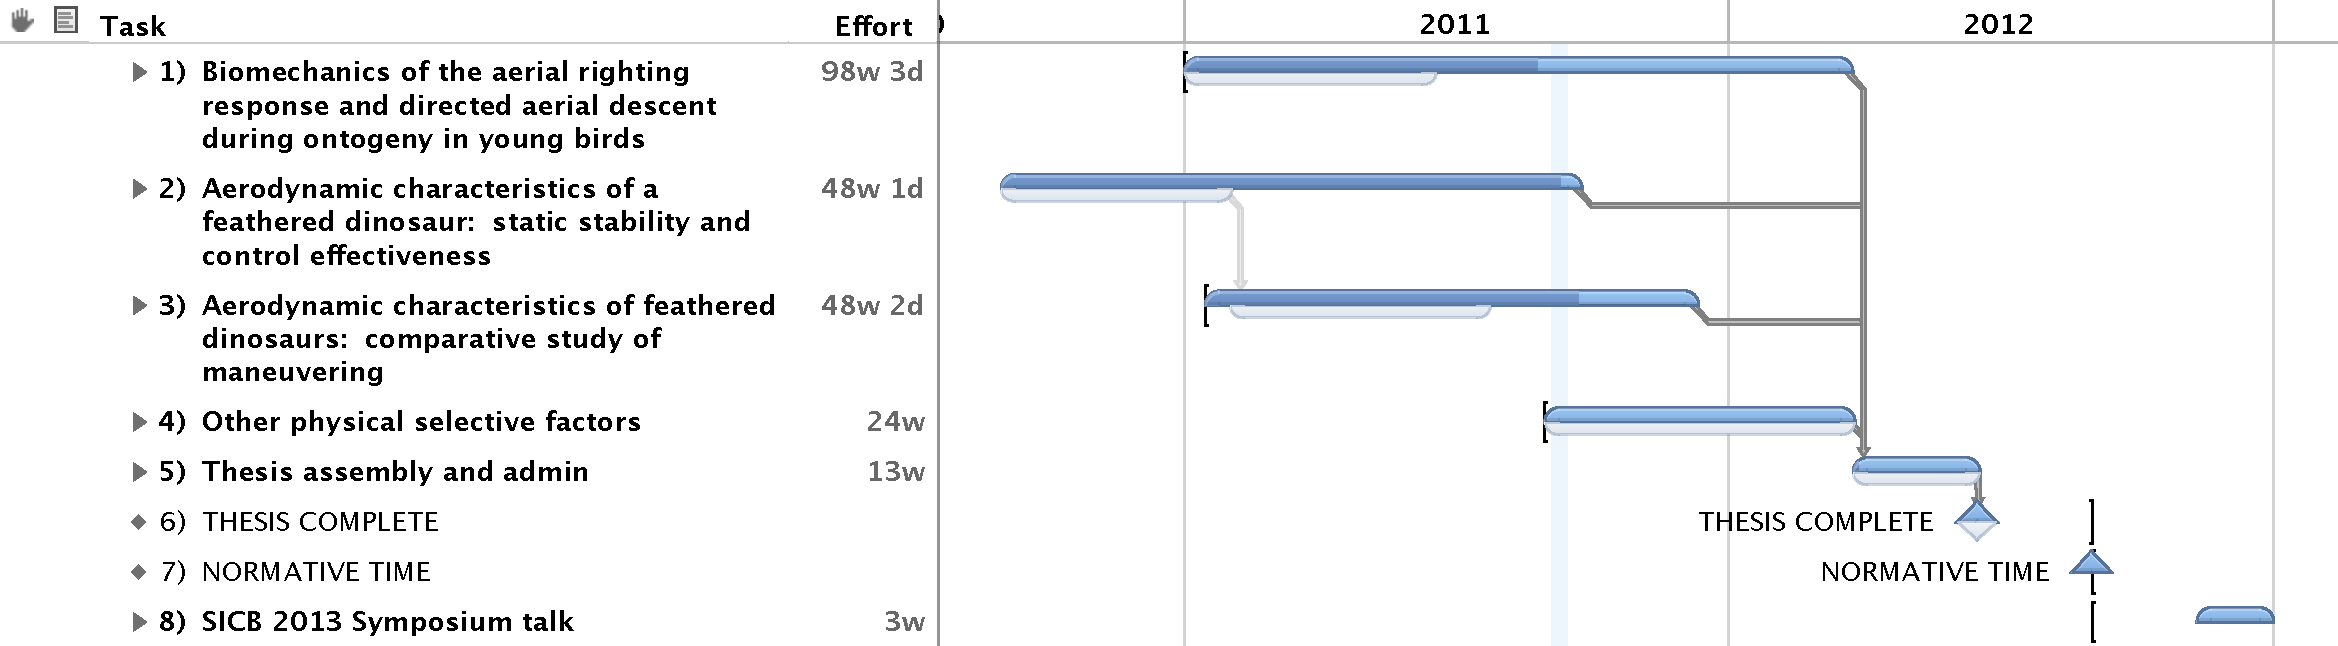
\includegraphics[width=9in]{figures/thesis-schedule-gantt.pdf}
\end{sidewaysfigure}

\rcsid{$Id$}
\rcsid{$Header$}
\rcskwsave{$Author$}
\rcskwsave{$Date$} 
\rcskwsave{$Revision$}

\chapter{Aerial righting and directed aerial descent during ontogeny in young birds}
\label{ch:1}
\index{maneuvering during ontogeny|(}

%\begin{abstract}
Abstract here  
%\end{abstract}

\section{Introduction}
\label{sec:1intro}

Write introduction here. 

%Introduction here\footnote{Target journal is \emph{J exp Biol}?} \citep{Dial:2003, Dial:2008}. The aerial righting reflex allows falling animals to reorient the body dorsoventrally, presumably to initiate gliding or parachuting and subsequent landing without injury using the legs.  
%
%Among vertebrates, aerial righting is likely widespread \citep{Dudley:2007} and others.  Aerial righting is achieved in cats and humans using zero-angular-momentum turns in which the body is twisted in sequence to rotate without external aerodynamic torque \citep{Kane:1969, Frohlich:1970, Liu:1985, Edwards:1986}.  In house geckos, aerial righting is similarly accomplished using torques generated by rapid rotation and nutation of the tail \citep{Jusufi:2008}.  (Fish? Frogs?)  
%
%Among terrestrial arthropods, aerial righting in stick insects (Zeng in preparation) is currently under study, and preliminary work indicates aerodynamic torques is dominates aerial righting (compared to inertial torques) in smaller stages.    
%
%(Has aerial righting been described in extant archosaurs, and have previous aerial righting studies considered size and aerodynamic effects?)  Do young birds possess an aerial righting reflex?  If so, how is aerial righting accomplished, and how does it change during ontogeny? 
%
%Previous workers have used the Chukar Partridge (\Alectorischukar), a ground-dwelling game bird native to Asia but imported to the US, as a model system to explore the use of the wings to assist incline running.  For comparison to this existing data set, chukars are a logical candidate for these experiments.  Alternative study organisms could include chickens or ducks (readily available from agricultural sources and able to be re-homed following experiments) or other birds in families that have evolved flightlessness (Ratites, penguins, kakapo parrots) or compromised flight abilities (various other running galliforms, puffins, cormorants).  However, unfortunately, unlike in stick insects, none of these has reversed the wing loss.  Another possibility is those birds for whom directed aerial descent in chicks is ecologically relevant (tree-nesting birds like murrelets or wood ducks). 

\section{Methods and materials}
\label{sec:1methods}

\subsection{Study animals}
A total of 29 Chukar Partridges (\Alectorischukar) in five batches, $x$ male and $y$ female, aged one day-post-hatching (dph), were obtained by hatching eggs from a local game bird farm (Fall Creek Game Birds; Felton, CA).  Clean, unwashed eggs were placed in a forced air incubator (HovaBator, GQF Manufacturing; Savannah, GA) equipped with a turning tray.  Eggs were held at \SI{37.5}{\celsius} (\SI{99.5}{\SIUnitSymbolDegree F}) for \SI{24}{\day}; turning was discontinued at \SI{21}{\day}.  Upon hatching, chicks were allowed to dry in the incubator for \SI{12}{\hour} and transferred to a brooder bin.  During the course of experiments, chicks were housed in \SI{53x38x30}{\centi\meter} brooder bins heated with two \SI{100}{\watt} floodlamps to maintain a brooder temperature of \SI{29.4}{\celsius} the first week, \SI{26.7}{\celsius} the second, and \SI{23.9}{\celsius} for subsequent weeks.  Birds were kept on wood shavings and offered crumbled chick starter rations (Purina; St.\ Louis, MO) and water \emph{ad libitum}.  Birds were also offered grit, freshly cut grass and mealworms. Chukars were studied at ages between \SIrange{1}{28}{dph}.  All handling of chicks and eggs was under protocols approved by the UC Berkeley Animal Care and Use Committee (ACUC).

To provide comparison with a species with slower wing development, a single batch of five Mallard Ducks (\Anasplatyrhynchos), 2 male and 3 female, was obtained as day-old-hatchlings from a local waterfowl farm (Metzer Farms; Gonzales, CA). Ducklings were housed on absorbent bedding in a large fiberglass tub and were fed on higher-protein waterfowl starter (Mazuri, Somewhere, NC).  Care of ducklings was similar to care for Chukar chicks, using protocols approved by the UC Berkeley ACUC.  Ducks were studied at ages between \SIrange{1}{70}{dph}.

For all birds, weights, lengths, and areas were measured daily to allow computation of wingspan, aspect ratio, area, and wing loading.  Birds were weighed using a digital scale (Scout Pro; Ohaus, Parsipanny, NJ).  Lengths and areas were obtained by restraining birds by hand against a gridded board and photographing using a digital camera (Canon PowerShot SD550); the photos were then digitized using ImageJ (NIH, Bethesda, MD). 

\subsection{Drop tests and manipulations}

Drop tests were conducted using methods similar to \citep{Jusufi:2008, Munk:2011, Zeng:2011}.  Birds were dropped in several different initial orientations (described below), from heights ranging between \SIrange{0.5}{2.5}{\meter}.  Aerial behaviors were captured using a suite of high speed and conventional digital video cameras.  High speed cameras consisted of between one and three cameras (AOS Technologies AG, Baden Daettwil, Switzerland; or Fastec Imaging, San Diego, CA) operated at \SI{500}{frames\per\second}, with one camera filming from the front and additional cameras filming from above or to the side.  Conventional cameras consisted of up to seven high definition (HD) cameras (FlipHD, Cisco Systems, San Francisco, CA), typically with four cameras filming at different angles from the front and additional cameras filming from above or to the side.  Camera pose and focus (intrinsic) parameters were estimated by filming a calibrated calibration object and using a Levenberg-Marquardt algorithm to minimize reprojection error, as described below.  Body positions were then digitized frame by frame using ImageJ (NIH, Bethesda, MD) and the resulting kinematics were analyzed as described below. 

The first batch of Chukars and the first batch of Mallard Ducks were dropped with upright, \ang{90}, and inverted (\ang{180}) orientations presented at random.  It was found that righting from the fully inverted position occurred very quickly in both (Section~\ref{sec:1results}, within \SI{4}{dph}) and that drops from upright position always remained upright.  Accordingly, subsequent drops were conducted only from the inverted position. 

In Chukar, manipulations to augment tail inertia were attempted by attaching plastic prosthetic long tails using veterinary wrap.  Tail augmentation was not successful\footnote{Birds tended to foul the prosthetic tail or mounting vet wrap with feces or groom it off.} and are not reported further here.  Symmetric and asymmetric clipping of wings (all remiges proximal to the outermost secondaries) and complete clipping of the tail (all retrices) were also performed at the end of all other runs.  

\subsection{Two-dimensional analysis}

As a first cut, a two-dimensional (2D) analysis was conducted to identify overall performance and changes during ontogeny.  2D analysis used a single side- or front view high-speed camera calibrated using scales within the image.  From the single view, 
the response time, righting angular velocity and angular position during the maneuver, vertical descent velocity, overall height lost, and success (\%) at righting were obtained. In additional, the righting method (discussed in Section~\ref{sec:1results}) was noted.  These were obtained for all ages.  

\subsection{Three-dimensional analyses}

For selected runs, a three-dimensional analysis was conducted to identify more precisely the onset of aerial behaviors and to determine the role of limb, tail, and body inertia in maneuvers.  

To perform three-dimensional analyses, a camera calibration technique was developed based on \cite{Munk:2011, Bradski:2008}. The calibration made use of homography transforms for multiple views of a two-dimensional chessboard calibration object to obtain camera poses (3D position and rotation), focus (intrinsic) parameters, and relative positions to one another.  With the camera parameters and with homologous points digitized in each image from each camera, a minimization routine was used to minimize the 2D reprojection error of the estimated 3D position. The method differs from \citep{Munk:2011} in the use of homography transforms and a 2D, repositionable calibration object compared to the large and fixed frame of \citep{Munk:2011}; this makes the method here more field-portable and easy to setup.  Details of the method are given in Appendix~\ref{app:cam}.  

The onset of aerial behaviors was detected by examining where the observed behaviors are no long well-described by a passive ballistic null model.  In the absence of any aerial behavior, the path of a falling object can be predicted using ballistics, \emph{i.e.\ } gravity, perhaps with drag.  The onset of aerial behavior is observed when we can detect behavior that deviates from this prediction.  To accomplish this, the likelihood of a given 3D trajectory was computed based on several candidate models for the behavior.  These were then compared using an Akaike Information Criterion (AIC):  
\begin{equation}
\mbox{AIC} = 2 k - 2 \ln(\mathcal{L})
\end{equation}
The candidate models are given by:
\begin{align}
\notag g_0:  x &= X_0 + \mathcal{N}(0,\sigma)& &\text{(stationary)}\\
\notag g_1:  x &= X_0 + V t + \mathcal{N}(0,\sigma)& &\text{(constant velocity)}\\
\notag g_2:  x &= X_0 + V t + \frac{1}{2}a t^2 + \mathcal{N}(0,\sigma)& &\text{(constant acceleration)}\\
\notag g_2':  x &= X_0 + V t - \frac{1}{2} \num{9.81} t^2 + \mathcal{N}(0,\sigma)& &\text{(Earth gravity)}\\
%\notag g_3:  x &= X_0 + V t + \frac{1}{2}a t^2 +\frac{1}{6}b t^3 + \mathcal{N}(0,\sigma)& &\text{(constant jerk)}\\
\notag g_3:  x &= X_0 + V t + X_1 e^{-t/\tau} + \mathcal{N}(0,\sigma)& &\text{(linear drag terminal velocity)}
\end{align}
 The derivation of these methods is given in Appendix~\ref{app:tdd}.

The relative role of inertia in accomplishing maneuvers was examined using a numerical method to predict how the maneuver would unfold in the absence of any aerodynamic forces.  The method is derived in Appendix~\ref{app:ang}.  Point masses are assigned 3D positions based on digitized body and limb positions obtained as described above.  These are then used in a forward calculation, to calculate the angular momentum and examine if it is constant (as would be predicted in a maneuver dominated by inertia) or if it is time-varying (as would be predicted where aerodynamic forces and torques are large).  The same data were also used in a reverse calculation, to obtain the whole body rotation that would result in a solely inertia case (i.e.\ in the case of a bird flying in a vacuum).  The methods here are superficially similar to \citep{Jusufi:2008, Bergou:2011} but avoid the need to derive explicit analytical expressions for multi-axis constrained linkages.  By numerically performing this calculation, this method is more applicable to a wider range of geometries and situations where the inertia acting to accomplish the maneuver is not straightforward to identify and lump into a single rotating element. 



\section{Results}
\label{sec:1results}
Write results here. 

\subsection{Morphometrics}
Figure~\ref{fig:1mass} shows chukar mass as a function of age.  
%Are there individual effects, yes probably.  Are there sex differences, I'm not sure. So maybe I'll have to plot the aerodynamic results versus mass, rather than age in days-post-hatching (doh), and will have to similarly convert the Dial stuff? 

\begin{figure}
\begin{center}
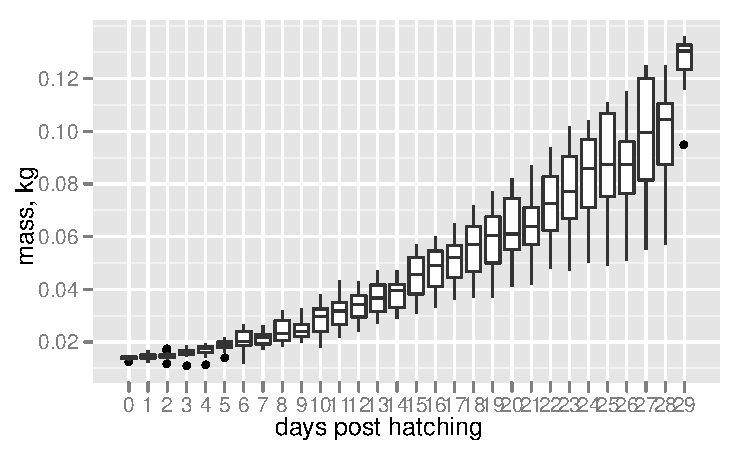
\includegraphics{figures/chukar-mass-boxplot.pdf}
\end{center}
\caption{Boxplot of chukar mass versus age. Explain what symbols are. Might be good to turn x-axis labels to avoid crowding.}
\label{fig:1mass}
\end{figure}

\subsection{Overall descent metrics}
\subsection{Onset of directed aerial descent}
\subsection{Inertial contribution to turns}


\section{Discussion}
\label{sec:1discussion}
Write discussion here. 

%\subsection{Evolutionary significance for the origins of bird flight}
%Birds lack a massive tail (unlike geckos) and their axial skeleton is stiffened by imbricated ribs and by the widespread fusion at the synsacrum (unlike mammals).  I would expect the avenues available to other vertebrate taxa for generating zero-angular-momentum turns are not present in birds, and dynamic models based on these other taxa should fail to predict the observed kinematics unless aerodynamic terms related to the wings or legs are added.  To test this further, patches could be used to augment areas (to simulate plumage changes with size held constant).  
%
%Theropod ancestors of birds had similar hips but lacked the rib cage stiffening; they also possessed long tails, and studies of falling bird chicks alone may not fully address this.  I may wish to test this further by manipulations to increase tail inertia by adding a boom similar to a theropod tail, or by testing aerial righting reflexes in other archosaurs (caimans).  This would provide a (somewhat weak) extant phylogenetic bracket for the presence of aerial righting in bird ancestors.
%
%The size-scaling of aerial righting ability may also be informative.  Many phylogenetic reconstructions of size in the clades leading to birds suggest they were small, perhaps small enough that both inertia and aerodynamics are important in the initial aerial righting given the phylogenetic constraints on axial body movement.  


\section{Acknowledgements}
We thank Dylan Marks for his assistance with filming.  We thank Luis Guillen and Kathy Moorhouse for their advice and assistance in raising birds.  We thank the Berkeley Center for Integrative Biomechanics Education and Research for the use of high speed cameras.  We thank Lindsay Waldrop, Kelly Dorgan, Yonatan Munk, Yu Zeng, Erica Kim, Marc Badger, Sofia Chang, Nir Sapir, Victor Ortega, and Marta Wolf for their analysis suggestions, assistance and support.  DE was supported by an NSF IGERT Fellowship and by a grant from the National and Berkeley local chapter of Sigma Xi.

\index{maneuvering during ontogeny|)}

% \bibliography{references/chukar} % copy all citations from this to main bibliography



\rcsid{$Id$}
\rcsid{$Header$}
\rcskwsave{$Author$}
\rcskwsave{$Date$} 
\rcskwsave{$Revision$}

\chapter{Aerodynamic characteristics of a feathered dinosaur shape measured using physical models: effects of form on static stability and control effectiveness}
\label{ch:2}
\index{Microraptor|(}

%\begin{abstract}
We report the effects of posture and morphology on the static aerodynamic stability and control effectiveness of physical models based loosely on a feathered dinosaur, \Microraptorgui, from the Cretaceous of China.  While some leg postures render \Mgui\ unstable, and thus quick to maneuver, others are stable, slower to maneuver but resistant to perturbation by wind gusts.  Depending on body posture, asymmetric leg positions can cause roll but have surprisingly little effect on yaw, while raising and lowering the tail or the hind limbs can alter pitch.  These results may help bound speculation and inform debate regarding \Mgui\ specifically, which has attracted much attention due to its leg and tail feathers.  Furthermore, while \Mgui\ lived after \Archaeopteryx\ and likely represents a side experiment with feathered morphologies, the general patterns of stability and control effectiveness as leg and tail morphologies are changed may help understand the evolution of flight control aerodynamics in vertebrates.  As further fossils with different morphologies or postures are found, these results could be applied in a phylogenetic context to understand potential biomechanical constraints on extinct flyers or gliders arising from the need to maneuver. 
%\end{abstract}

\section{Introduction}
The evolution of flight in vertebrates, and particularly in birds, is the subject of lively debate and considerable speculation.  Furthermore, flight ability of extinct vertebrates is often inferred from very simple parameters (such as lift and drag coefficients and glide angles \cite{Emerson:1990, Emerson:1990b}); these alone may not be sufficient as anything flying in a real environment will experience perturbations and need to maneuver around obstacles \cite{Dudley:2012}.  

Discoveries during the last decade of a diversity of feathered dinosaurs and early birds from the Cretaceous of Liaoning, China have led to considerable speculation about the roles that the feathers played on these extinct animals. Fossil forms are important in biomechanical studies because they may indicate ``missing links'', transitional forms within a lineage, between ancestral and derived, or they record ``experiments'' in form in side-branches; both are informative for questions of biomechanics.  Although we cannot observe the behavior of extinct animals, we can measure the aerodynamic forces on dynamically-scaled physical models in a wind tunnel to quantify the broader effects on performance of different postures and morphologies.  Since physical laws apply the same to all taxa, regardless of history, knowing about the physical implications of shape can suggest ``priors'' that would apply to anyone in the air. 
  
The Jiufotang Formation has been interpreted as a forest based on pollen data and plant fragments \cite{someone}.  The inference that \Mgui\ was arboreal solely based on pollen is not terribly strong, given that not everything that lives in a forest lives in the trees and that processes after death (taphanomy) that occur during fossilization also tend to wash everything together.  However, quite many things in forests make use of the trees even if they don't appear particularly arboreal. In addition, the vertebrate diversity includes stuff as well as numerous feathered theropod dinosaurs and early birds \cite{someone}, many with small size and similar feathered forms, suggesting that at least some might have been in the trees and performing aerial behaviors even if \Mgui\ was not. Somehow this needs to be dealt with. See Xu letter and Zhou letter in Nature. 
  
We used such models, loosely based on \Microraptorgui\ (Figure~\ref{fig:mgui}), a cat-sized dromaeosaur with flight feathers on its forelimbs, hindlimbs, and tail, enabling us to investigate effects of diverse aerodynamic surfaces in the aft/posterior of a body.  By measuring not just lift and drag, but also side forces and moments in pitch, roll, and yaw, we can assess static aerodynamic stability (tendency to experience righting torques when perturbed) and control effectiveness (moments generated by motions of control surfaces), both of which affect the ability to maneuver while gliding or parachuting through a complex forest habitat. 
\begin{figure}
%\includegraphics[width=6in]{figures/fossil/Microraptor-IVPP-V13352-5cm.jpg}
\caption{%
{ \Microraptorgui\ \cite{Xu:2003}, a dromaeosaur from the Cretaceous Jiufotang Formation of Liaoning, China.}  Holotype specimen IVPP V13352, scale bar \SI{5}{\centi\meter}.  Notable features include semilunate carpal bones, a boomerang-shaped furcula, a shield-shaped sternum without a keel, uncinate processes on the ribs, unfused digits, an intermediate angle of the scapulocoracoid, and a long tail of roughly snout-vent length.  In addition, there are impressions of feathers on the forelimbs, hindlimbs, and tail.%
}
\label{fig:mgui} 
\end{figure}

We compared the lift, drag, and side forces, and the pitch, roll, and yaw moments on models with vs. without leg feathers, and we tested the models in different symmetric and asymmetric postures that have been proposed by various researchers.  In some cases leg feathers had no effect, and in others they did (e.g. leg feathers reduced drag for some postures at some angles of attack). Therefore, whether or not leg feathers affected gliding, parachuting, or maneuvering performance depended on the posture and orientation of the dinosaur.  These results will contribute to our understanding of the role of aerodynamic surfaces aft of a gliding animal's center of mass.

This is the first of two paper dealing with the \Mgui\ aerodynamics.  In this paper we do some stuff.  In the second paper, we will...

\subsection{Previous work with models}

Further lit review add in later.  Gatesy and Dial 1996 looked at Archaeopteryx tails, Longrich did some maneuvering calcs based on McCay; Chatterjee and Templin did purely computer model of phugoid dynamics; Nova guys, Alexander (2010) did full scale flying models.  Our methods are most similar to Xu Jenkins Breuer Nova and Alexander 2010.  

\subsection{Additional engineering background}

Multiple surfaces in tandem might be expected to have large impacts for maneuvering.  In engineering practice, submarine snap rolls can be caused by interactions between the sail and rudder (citation).  In biology, interactions between median or paired fins can enhance maneuvering in fish; the four-(or more) flipper planform is widely seen in aquatic creatures but seems largely absent from fliers (exceptions frogs, four-winged flying fish, any others?). Why?  

Changes in flight performance from being a crappy flier to a good flier might be expected to have changes in glide angle or AOA associated with them.  High AOA aerodynamics can be vastly different from low AOA, with shifts in stability expected.  Shifts in stability at high AOA is responsible for crashes (citations). 

In engineering practice there is also the concept of control plane reversal, in which a control surface acts the opposite of what it ``normally'' does; for example, at low speed ships rudders or planes acting opposite to their normal direction has caused collisions of cruise ships (citations) others (citations), 





% You may title this section "Methods" or "Models". 
% "Models" is not a valid title for PLoS ONE authors. However, PLoS ONE
% authors may use "Analysis" 
\section{Materials and Methods}

\subsection{Models and postures}
Scale models of \Mgui\ (%mass \SIrange{1}{1.4}{\kilo\gram}, 
snout-vent length \SI{8}{\centi\meter}) were constructed from published reconstructions and photographs \citep{Xu:2003, Chatterjee:2007, Nova}.  The models are shown in Figure~\ref{fig:model}A.  Model construction was guided by dissection of Starlings (\emph{Sturnus vulgaris}), reference to preserved specimens of birds, bird wings, and lizards, teaching casts of \Archaeopteryx, and illustrated textbooks on vertebrate functional morphology and vertebrate paleontology \citep{Liem:2000, Benton:1997}.  Photographs of the \Mgui\ holotype IVPP V13352 were printed on a laser printer (Xerox, Norwalk, CT) at full scale and at model scale to further guide model construction.  %However, no member of our research team has ever had the opportunity to personally examine an \Mgui\ fossil or cast.  
\begin{figure}
\caption{%
{ Physical models of \Mgui, wingspan \SI{20}{\centi\meter}, snout-vent-length \SI{8}{\centi\meter}.}  Reconstruction postures (a-d) used for constructing physical models:  a, sprawled, after \citep{Xu:2003};  b, tent, after \citep{Nova}; c, legs-down, after \citep{Nova};  d, biplane, after \citep{Chatterjee:2007}. Additional manipulations (e-h): e, sprawled without leg or tail feathers; f, tent without leg or tail feathers; g, example asymmetric leg posture with \ang{90} leg mismatch \emph{arabesque}; h, example asymmetric leg posture with \ang{45} dihedral on one leg \emph{d{\'e}gag{\'e}}.%
}
\label{fig:model}
\end{figure}

Models were built on an aluminum plate with polymer clay (Polyform Products Co., Elk Grove, IL) to fill out the body using methods described in \citep{Koehl:2012}.  Removable tails and heads, to allow repositioning, were constructed using polymer clay over steel rods.  The forelimbs were constructed by bending 26-gauge steel wire scaled to the lengths of the humerus, radius and ulna, and digits as seen in published photographs of the holotype.  Similarly, hindlimbs were constructed with wire scaled to the lengths of the femur, tibiotarsus, tarsometatarsus, and digits.  For the appendages and tail, feathered surfaces were modeled using paper and surgical tape (3M, St.\ Paul, MN) stiffened by addition of monofilament line at the locations of the individual feather rachises.  This method of creating wing surfaces was compared to wings with craft feathers individually sewn onto them and seen to provide equivalent results\citep{Koehl:2012}.  In addition, models of Anna's Hummingbirds (\emph{Calypte anna}) constructed using the same techniques have been shown to faithfully reproduce the aerodynamic properties of diving hummingbirds (Evangelista, in preparation).  

Model reconstruction postures (Figure~\ref{fig:model}B-E) were chosen based on those previously published \citep{Xu:2003, Chatterjee:2007, Nova}.  Some of these postures are anatomically dubious; in particular the sprawled posture drawn in \citep{Xu:2003} has been criticized because of interference between the trochanter on the femur and the surrounding structures of the ilium and ischium \citep{someone}, while a feasible mechanism for maintaining feathers in the biplane / muffed feet posture of \citep{Chatterjee:2007} under load has never been proposed.  We also tested models in postures more strongly inferred for theropods, including a legs-down posture with no more than \ang{45} leg abduction \citep{Nova}, and a tent posture in which the legs are extended caudad with the feathered surface extending over the proximal part of the tail.  %Xu never intended the sprawled posture as an actual reconstruction per se. \citep{Xu:2005a} check this, and in the absence of fossil material illustrating otherwise there is no reason to assume extraordinary hip anatomy not seen in any other theropod.  

We recognize that some of the reconstruction postures are less feasible than others.  The approach taken here is to test all previously proposed reconstructions, in order to examine the aerodynamic implications of these shapes from a purely physical standpoint.  With the uncertainties inherent in applying a physical modeling approach to an extinct animal with only a single published skeleton, statements about aerodynamic performance in \Mgui\ should always be taken with a grain of salt.  %There are other reasonable things said in numerous letters that ought to be mentioned here. 

%\subsection*{Conditions for dynamic similarity}
%To achieve dynamic similarity in these models, it would be nice to match the Reynolds number ($\mbox{Re} = uL/\nu$), the nondimensional ratio of viscous to inertial forces.  Based on pilot studies we estimated $\mbox{Re}$ for the full scale \Mgui\ to be approximately \num{200000}.   Limitations on the wind tunnel size and speed required the Reynolds number of the model to be \num{32000}.  How bad is this? Check that correct scales are being used and that the old uraps did the calculation right. 
%\input{tables/similarity.tex}

\subsection{Force measurements}
As described in \citep{Koehl:2012}, models were mounted on a six-axis force transducer (Nano17, ATI Industrial Automation, Apex, NC), which was in turn mounted on a 1/4-20 threaded rod damped with rubber tubing, and attached to a tripod head used to adjust angle-of-attack.  The force sensor and sting exited the model on the right side of the body mid-torso at approximately the center of mass.

Wind tunnel tests were conducted in an open jet wind tunnel with an \SI{15 x 15 x 18}{inch} (\SI{38.1 x 38.1 x 45.7}{\centi\meter}) working section used previously for studies of gliding frogs \citep{McCay:2001, McCay:2001a}.  Tunnel speed was controlled using a variable autotransformer (PowerStat, Superior Electric Company, Bridgeport, CT) and monitored using a hot wire anemometer (Series 2440, Kurz Instrument Co., Monterey, CA).  

Force transducer readings were recorded at \SI{1000}{\hertz} sampling frequency using a National Instruments 6251 data acquisition card (National Instruments, Austin, TX).  Raw measurements were rotated from a frame fixed to the model to one aligned with the wind tunnel and flow using the angle-of-attack.  Transformed measurements were then averaged over a one-minute recording.  For each measurement, wind tunnel speed $v$ was recorded and used to compute Reynolds number ($\mbox{Re} = vL/\nu$, $\nu = \SI{15.e-6}{\meter\squared\per\second}$).  The sign convention for forces and moments is shown in Figure~\ref{fig:signconvention}

\begin{figure}
%\includegraphics[width=4in]{figures/sign-conventions/Pitch-signs.pdf}
%\includegraphics[width=2in]{figures/sign-conventions/yaw-signs.pdf}
\caption{%
{Sign conventions, rotation angles, and definitions for model testing, after \citep{Emerson:1990b,McCay:2001,McCay:2001a,McCormick:1995}.}%
}
%\caption{}
\label{fig:signconvention}
\end{figure}  

Aerodynamics forces and moments were  normalized to obtain nondimensional coefficients according to the following (rewrite this to use notation from \citep{McCormick:1995}): 
\begin{equation}
\mbox{lift} = C_L 0.5 \rho u^2 A_p
%C_L = \frac{\mbox{lift}}{1/2 \rho u^2 A_p}
\end{equation}
\begin{equation}
\mbox{drag} = C_D 0.5 \rho u^2 A_p
%C_D = \frac{\mbox{drag}}{1/2 \rho u^2 A_p}
\end{equation}
\begin{equation}
\mbox{side force} = C_S 0.5 \rho u^2 A_p
%C_S = \frac{\mbox{side force}}{1/2 \rho u^2 A_p}
\end{equation}
\begin{equation}
\mbox{pitching moment} = C_m 0.5 \rho u^2 A_p \lambda_{SVL}
%C_m = \frac{\mbox{pitching moment}}{1/2 \rho u^2 A_p \lambda_{SVL}}
\end{equation}
\begin{equation}
\mbox{rolling moment} = C_r 0.5 \rho u^2 A_p \lambda_{SVL}
%C_r = \frac{\mbox{rolling moment}}{1/2 \rho u^2 A_p \lambda_{SVL}}
\end{equation}
\begin{equation}
\mbox{yawing moment} = C_y 0.5 \rho u^2 A_p \lambda_{SVL}
%C_y = \frac{\mbox{yawing moment}}{1/2 \rho u^2 A_p \lambda_{SVL}}
\end{equation}
where $\rho=\SI{1.204}{\kilo\gram\per\meter\cubed}$ is the air density, $A_p$ is the model planform area, and $\lambda_{SVL}$ is the snout-vent length of the model.  To allow comparisons among models, a single, consistent baseline configuration is needed.  Accordingly, nondimensional coefficients are referenced to the planform area of the four-winged, sprawled position originally proposed in \citep{Xu:2003} unless specially noted.  The questions of interest for this study are tied to the absolute value of forces and moments produced and differences that occur from the same animal in different postures; our choice of normalization preserves these distinctions in most cases.  

%MK:  I do remember deciding that we should use the full plan area of the body in the sprawled posture for all the postures with four wings.  I'm glad you let me know that you used the four-wing plan area to calculate the coefficients for the two-winged models.

%DE: 
%\emph{If we hit a case where we want to see area differences, we can show raw forces and coefficients using are but that is probably irrelevant for this study.  It comes up in Draco studies of no - half - full - double wing but is not important to the questions here.}

\subsection*{Static stability coefficients}
To assess static stability, we calculated nondimensional static stability coefficients from fixed-wing aircraft stability and control theory \citep{McCormick:1995} and previously used in studies of gliding frogs \citep{McCay:2001, McCay:2001a}.

The pitching stability coefficient $C_{m,\alpha}$ is defined as \citep{McCay:2001}
\begin{equation}
\partial C_m = C_{m,\alpha} \partial\alpha
%C_{m,\alpha} = \frac{\partial C_m}{\partial\alpha}
\end{equation} 
where $\alpha$ is the angle-of-attack and $C_m$ is the pitching moment coefficient as defined above. It is the local slope of the pitching moment curve, and is thus an indication of the sense (restoring or non-restoring) and magnitude of the torque generated in response to a perturbation in angle-of-attack.  If $C_{m,\alpha}<0$, the response torque will be opposite the direction of perturbation; this is the condition for static stability. 

Similarly, for roll:
\begin{equation}
\partial C_r = C_{r,\phi} \partial\phi
%C_{r,\phi} = \frac{\partial C_r}{\partial\phi}
\end{equation}
where $\phi$ is the roll angle and $C_{r,\phi}<0$ is the condition for static stability in roll. By symmetry, models at zero angle-of-attack have neutral rolling stability, and we did not calculate roll stability for most cases.

For yaw, 
\begin{equation}
\partial C_y = C_{y,\psi} \partial\psi
%C_{y,\psi} = \frac{\partial C_y}{\partial\psi}
\end{equation}
where $\psi$ is the yaw angle and $C_{y,\psi}<0$ is the condition for static stability in yaw (also known as directional stability).  

Pitching stability coefficients were obtained from angle-of-attack ($\alpha$) runs taken from \ang{-15} to \ang{90} at \ang{5} increments.  Yawing stability coefficients were obtained from yaw angle ($\psi$) runs from \ang{-30} to \ang{30} at \ang{10} increments. For each series, central differences were used to estimate the slopes at each point for each replicate run.   

\subsection{Control effectiveness}
We also calculated nondimensional control effectiveness coefficients using methods from aerodynamic engineering \citep{Etkin:1996} used in previous studies of gliding frogs \citep{McCay:2001a}. In general, control effectiveness for a control surface whose angular orientation relative to the flow can be changed is the partial derivative of the moment generated with respect to the angle. High control effectiveness means a large amount of moment generated for a small movement of the surface.  

We calculated the pitching control effectiveness for the tail, forewings, and legs as follows:
\begin{equation}
\partial C_m = C_{m,\delta} \partial\delta
%C_{m,\delta} = \frac{\partial C_m}{\partial\delta}
\end{equation}
where $\delta$ is the angle of the control surface in question.  Similarly, we calculated yawing control effectiveness for these surfaces as follows:
\begin{equation}
\partial C_y = C_{y,\delta} \partial\delta
%C_{y,\delta} = \frac{\partial C_y}{\partial\delta}
\end{equation}
as well as rolling control effectiveness for asymmetric movements of the wings and legs:
\begin{equation}
\partial C_r = C_{r,\delta} \partial\delta
%C_{r,\delta} = \frac{\partial C_r}{\partial\delta}
\end{equation}

\subsection{Other flight performance metrics}
To allow comparison with previous studies, two additional measures of maneuvering performance we computed: the banked turn maneuvering index and crabbed turn maneuvering index \citep{Emerson:1990b, McCay:2001, McCay:2001a}.  The banked turn maneuvering index assumes turns accomplished by banking is computed in two ways, both of which assume that some component of lift generated is used to provide the force necessary for turning:
\begin{equation}
MI_{\mbox{banked,1}} = \frac{C_{L,\mbox{max}}}{mg/A_P}
\end{equation}
after \citep{Emerson:1990b} (note this is not a nondimensional index), and 
\begin{equation}
MI_{\mbox{banked,2}} = \frac{L \cos{\phi}}{mg}
\end{equation}
where $\phi=\ang{60}$ is arbitrarily chosen with no reasonable basis for picking it, after \citep{McCay:2001, McCay:2001a}.  Similarly, for crabbed turns, a nondimensional index is the horizontal component of side force normalized by body weight \citep{McCay:2001, McCay:2001a}:
\begin{equation}
MI_{\mbox{crabbed}} = \frac{F_{\mbox{side}} \sin{\psi}}{mg}
\end{equation}
again with $\psi=\ang{60}$ arbitrarily chosen based on frogs \citep{McCay:2001,McCay:2001a}. 

Actually the indices here from \citep{Emerson:1990b, McCay:2001, McCay:2001a} are stupid; they are just recast versions of other numbers that are more informative without being mucked around with. 

We also calculated several flight performance metrics not immediately tied to maneuvering \citep{McCay:2001, McCay:2001a, Emerson:1990, Emerson:1990b}. As a measure of horizontal glide performance, we computed $(C_L/C_D)_{\mbox{max}}$ for each posture \citep{Emerson:1990b}. Minimum glide speed, a measure of the ease of which gliding can be initated, was also computed as $U_{\mbox{min}} = [2mg /(A_P \rho C_L)]^{1/2}$ \citep{Emerson:1990b}. As a measure of parachuting ability, we also compared $D_{90}$, the full scale drag for parachuting \citep{Emerson:1990b}, as well as a nondimensionalized parachuting index $D_{90}/mg$.  

%\subsection*{Agility and maneuverability}
%McCay quantified agility as the time (latency) to achieve an arbitrary \ang{60} change in yaw and used live animal kinematics or benchmarked simulations to estimate it \citep{McCay:2001a}.  Similarly, McCay defined maneuverability (other than the maneuvering indices above) as turning radii from live animal kinematics or benchmarked simulations \citep{McCay:2001a}.  Without a live animal or a simulation with sufficient benchmarking to have some confidence in its predictions, we did not compute either of these quantities for \Mgui.   

%\subsection*{Reynolds number sweep}
%A sweep in speed was conducted to check how much coefficients varied with speed.  

%\subsection*{Estimation of mass and gravitationally induced moments}
%The mass of a live \Mgui\ was estimated by scaling using data from some sources.  Fill in more later.  To estimate gravitationally induced moments and the location of the center of mass, mass of some body parts were scaled from birds and dimensions and positions estimated from fossil and reconstruction position.  Fill in more later. 






% Results and Discussion can be combined.
\section{Results}
During the fall of 2010, we collected a dataset of 12,810 measurements for 180 combinations of postures and positions.  The raw data require approximately 5.3 GB of storage.  The work was accomplished during approximately 350 hours of wind tunnel time by a team of ten undergraduates led by one graduate student.

For the plots given here, color represents the base posture: red for sprawled, blue for tent, green for biplane, and purple for down.  All sign conventions are as in \citep{McCay:2001} and as shown in Fig~\ref{fig:signconvention}.  Symbols, where used, represent variations in position from the base posture, such as movement of legs, wings, or tail. All units are SI unless otherwise noted. 

%\subsection*{Mass, center, and gravitational moment estimates?}
%\subsection*{Method and model benchmarking?}
%Raw force data, papers versus feather, tunnel speed calibration, Reynolds number sweep mostly covered in stupid ICB paper.

\subsection{Baseline longitudinal plane aerodynamic data and effects of posture and the presence/absence of leg and tail feathers}
Fig~\ref{fig:coeffsvsaoa} gives the nondimensional coefficients of lift, drag, and pitching moment for \Mgui with full feathers.  
\begin{figure}
a %\includegraphics{figures/Gliding/pitch-stability/basicClvsaoa.pdf}
b %\includegraphics{figures/Gliding/pitch-stability/basicCdvsaoa.pdf}
c %\includegraphics{figures/Gliding/pitch-stability/basicClvsCd.pdf}
d %\includegraphics{figures/Gliding/pitch-stability/basicCmvsaoa.pdf}
\caption{{ Nondimensional coefficients for all models.}  Red is sprawled, blue is tent, green is biplane, purple is down. $\alpha$ from \ang{-15} to \ang{90} in \ang{5} increments, with 5 or more replicates per treatment. a: Lift coefficent. b: Drag coefficient. c: Lift drag polars.  d: Pitching moment coefficient.}
\label{fig:coeffsvsaoa}
\end{figure}
Scaling with the coefficients, the full scale forces for \Mgui\ at \SI{12}{\meter\per\second} are plotted in Fig~\ref{fig:fsall}.
\begin{figure}
a %\includegraphics{figures/Gliding/pitch-stability/basicfsLvsaoa.pdf}
b %\includegraphics{figures/Gliding/pitch-stability/basicfsDvsaoa.pdf}
c %\includegraphics{figures/Gliding/pitch-stability/basicfsLvsD.pdf}
d %\includegraphics{figures/Gliding/pitch-stability/basicfsMvsaoa.pdf}
\caption{{ Full scale forces and moments for \Mgui\ at \SI{12}{\meter\per\second}}.  Red is sprawled, blue is tent, green is biplane, purple is down. $\alpha$ from \ang{-15} to \ang{90} in \ang{5} increments, with 5 or more replicates per treatment. a: Full scale lift at \SI{12}{\meter\per\second}, all models. This figure must be annotated to show the band of \Mgui\ body weight. b:  Full scale drag at \SI{12}{\meter\per\second}, all models. This figure must be annotated to show the band of \Mgui\ body weight. c: Lift-drag polars. d: Full scale pitching moment at \SI{12}{\meter\per\second} versus angle of attack, all models.}
\label{fig:fsall}
\end{figure}
For comparison with previous work \citep{Emerson:1990b}, various other gliding performance metrics are compared in figures~\ref{fig:EKcomparisons1} and \ref{fig:EKcomparisons2}.  
\begin{figure}
a %\includegraphics{figures/Gliding/pitch-stability/liftdragratio.pdf}
b %\includegraphics{figures/Gliding/pitch-stability/glideangle.pdf}
c %\includegraphics{figures/Gliding/pitch-stability/Umin.pdf}
%d \includegraphics{figures/Gliding/pitch-stability/Upropelled.pdf}
d %\includegraphics{figures/Gliding/pitch-stability/Uterm.pdf}
e %\includegraphics{figures/Gliding/pitch-stability/pitchstab.pdf}   
\caption{ Red is sprawled, blue is tent, green is biplane, purple is down. $\alpha$ from \ang{-15} to \ang{90} in \ang{5} increments, with 5 or more replicates per treatment. a: Lift to drag ratio. b: Glide angle. c: Minimum glide speed. d: Terminal velocity (assuming stability). e: Pitching stability coefficient (note pitching moment must also be zero for stable equilibrium).}
\label{fig:EKcomparisons1}
\end{figure}
\begin{figure}
a %\includegraphics{figures/Gliding/emerson-koehl-1/ClCdvsposture.pdf}
b %\includegraphics{figures/Gliding/emerson-koehl-1/Uminvsposture.pdf}
c %\includegraphics{figures/Gliding/emerson-koehl-1/D90vsposture.pdf}
\caption{%
{ Comparison of simple glide metrics after \citep{Emerson:1990b} suggests the metrics are not informative.}
Red is sprawled, blue is tent, green is biplane, purple is down.%
a:  Maximum lift to drag ratio, by posture, without regard to stability.  \citep{Emerson:1990b}'s minimum ratio is never achieved because the models are not stable at the point where $L/D$ is maximum.  There is no difference in maximum lift to drag ratio among postures (Kruskal-Wallis, $P=0.1740$). b: Minimum glide initiation speed, by posture, without regard to stability. The minimum speed is never achieved because the models are not stable at the point where $U_{min}$ is lowest.  There is no difference in $U_{min}$ among postures (Kruskal-Wallis, $P=0.575$).  c:  Parachuting drag, by posture, without regard to stability. This drag is never achieved because the models are not stable at a \ang{90} angle-of-attack.  There are significant differences in $D_{90}$ among postures (Kruskal-Wallis, $P=\num{9.2e-5}$); sprawled position has higher parachuting drag.}
\label{fig:EKcomparisons2}
\end{figure}
A Reynolds number sweep (Fig~\ref{fig:Reynoldsnothing}, Table~\ref{tbl:similarity}) was also conducted to check for scale effects. 
\begin{figure}
%\includegraphics{figures/Methods/reynolds-sweeps/liftvsRe.pdf}\\
%\includegraphics{figures/Methods/reynolds-sweeps/dragvsRe.pdf}\\
%\includegraphics{figures/Methods/reynolds-sweeps/pitchvsRe.pdf}
\caption{Reynolds number sweeps for lift, drag, and pitch coefficients. There are not large changes in aerodynamic coefficients over the ranges shown here.  This is similar to what is seen in \emph{Draco} lizard and Anna's Hummingbird (\emph{Calypte anna}) models. The coefficients are roughly constant in the range of \emph{\dag Archaeopteryx} and are constant enough for these results to be applicable to \emph{\dag Microraptor}.}
\label{fig:Reynoldsnothing}
\end{figure}
%\input{tables/similarity.tex}

%\subsection*{Effect of leg and tail feathers}
The effects on longitudinal plane coefficients of the presence or absence of leg and tail feathers is shown in Fig~\ref{fig:feathers1} and \ref{fig:feathersEK}, as a ``what if'' examination of morphological changes that may put the results in context.  
\begin{figure}
a %\includegraphics{figures/Gliding/adrian-eric-pitch-stability2/aeClvsaoa.pdf}
b %\includegraphics{figures/Gliding/adrian-eric-pitch-stability2/aeCdvsaoa.pdf}
c %\includegraphics{figures/Gliding/adrian-eric-pitch-stability2/aeClvsCd.pdf}
d %\includegraphics{figures/Gliding/adrian-eric-pitch-stability2/aeLDvsaoa.pdf}
e %\includegraphics{figures/Gliding/adrian-eric-pitch-stability2/aeCmvsaoa.pdf}
f %\includegraphics{figures/Gliding/adrian-eric-pitch-stability2/aepitchstab.pdf}
\caption{{ Presence or absence of leg and tail feathers can drastically alter longitudinal plane aerodynamics.}.  Sprawled and tent postures with and without feathers. All coefficients shown versus angle-of-attack. a: Lift coefficient.  Stall occurs at higher angle-of-attack when leg feathers are present. b: Drag coefficient.  Leg feathers increase drag at high angle-of-attack, improving parachuting performance. c: Lift coefficient versus drag coefficient. d: Lift to drag ratio. Lift to drag ratio is improved slightly without the additional drag and less-efficient lift generation of hind wings. e: Pitching moment coefficient. Without leg feathers, stability is not achieved in either posture. f: Pitching stability coefficient.}
\label{fig:feathers1}
\end{figure}
\begin{figure}
%\includegraphics{figures/Gliding/emerson-koehl-2/ClCdvsposturefeathers.pdf}
%\includegraphics{figures/Gliding/emerson-koehl-2/Uminvsposturefeathers.pdf}
%\includegraphics{figures/Gliding/emerson-koehl-2/D90vsposturefeathers.pdf}
\caption{{ Presence or absence of leg and tail feathers has effects on \citep{Emerson:1990b} metrics}.  a:  Maximum lift to drag ratio, by sprawled and tent postures with and without feathers.  The maximum lift to drag ratio for tent without leg or tail feathers is significantly higher than for other postures (ANOVA, $P < 0.003$), however, this improvement is never achieved because the tent posture is never stable without leg feathers. b:  Minimum glide speed, by sprawled and tent postures with and without feathers.  There are no differences in minimum glide speed between postures (ANOVA, $P > 0.08$). c:  Parachuting drag, by sprawled and tent postures with and without feathers.  There are significant differences in parachuting drag between postures (ANOVA, $P < 0.04$), however, the straight-down parachuting position is not stable in any posture. }
\label{fig:feathersEK}
\end{figure}


\subsection*{A closer look at stability, control effectiveness, and maneuvering}
Perhaps from here and below will go in Part 2???
\subsection{Yaw stability}
\begin{figure}
%\includegraphics{figures/Gliding/yaw-stability/yaw-0/Cyawvshdg.pdf}\\
%\includegraphics{figures/Gliding/yaw-stability/yaw-0/Csidevshdg.pdf}
\caption{At \ang{0} angle-of-attack, there are clear differences in yaw stability between postures.  In particular, with legs down, the legs strongly act as weathervanes to stabilize the body in yaw. }
\label{fig:yaw1}
\end{figure}
\begin{figure}
\ang{0} %\includegraphics{figures/Gliding/yaw-stability/yaw-0/Cyawvshdg.pdf}\\
\ang{60} %\includegraphics{figures/Gliding/yaw-stability/yaw-60/Cyawvshdg.pdf} \\
\ang{90} %\includegraphics{figures/Gliding/yaw-stability/yaw-90/Cyawvshdg.pdf} \\
\caption{There are also clear differences in yaw stability at different angles-of-attack. At \ang{0}, some postures are more stable in yaw than others.  At \ang{60}, postures that were stable at \ang{0} may go unstable, such as tent posture.  At \ang{90}, all postures are marginally stable due to symmetry. }
\label{fig:yaw2}
\end{figure}
\begin{figure}
\ang{0} %\includegraphics{figures/Gliding/adrian-eric-yaw-stability/aeyaw-0/aeCyawvshdg.pdf}\\
\ang{60} %\includegraphics{figures/Gliding/adrian-eric-yaw-stability/aeyaw-60/aeCyawvshdg.pdf} \\
\ang{90} %\includegraphics{figures/Gliding/adrian-eric-yaw-stability/aeyaw-90/aeCyawvshdg.pdf} \\
\caption{The differences in yaw stability at different angles-of-attack also depend on the presence or absence of leg feathers. At \ang{0}, some feathered-leg postures are more stable in yaw than others.  At \ang{60}, postures that were stable at \ang{0} may go unstable, such as tent posture with leg feathers.  At \ang{90}, all postures are marginally stable due to symmetry. }
\label{fig:yaw3}
\end{figure}




\subsection{Control effectiveness of tail, symmetric wing and leg movements}
\begin{figure}
%\includegraphics{figures/Gliding/control-effectiveness-1/tail/biplane/Clvsaoa.pdf} \\
%\includegraphics{figures/Gliding/control-effectiveness-1/tail/biplane/Cmvsaoa.pdf} \\
\caption{Tail control effectiveness for biplane posture for tail angles of \ang{-15} (down triangle), \ang{0} (square), and \ang{+15} (up triangle).  At low angle-of-attack, tail up produces a nose up moment relative to zero tail angle, while tail down produces a nose down moment relative to zero tail angle.  The small effect on lift suggests the tail is primarily effective because of moments generated by its long length.}
\end{figure}
\begin{figure}
%\includegraphics{figures/Gliding/control-effectiveness-1/tail/down/Clvsaoa.pdf} \\
%\includegraphics{figures/Gliding/control-effectiveness-1/tail/down/Cmvsaoa.pdf} \\
\caption{Tail control effectiveness for down posture for tail angles of \ang{-15} (down triangle), \ang{0} (square), and \ang{+15} (up triangle).  At low angle-of-attack, tail up produces a nose up moment relative to zero tail angle, while tail down produces a nose down moment relative to zero tail angle.  At high angle of attack, the tail experiences reversal in which tail down produces nose up moments / tail up produces nose down moments.}
\end{figure}
\begin{figure}
%\includegraphics{figures/Gliding/control-effectiveness-1/tail/sprawled/Clvsaoa.pdf} 
%\includegraphics{figures/Gliding/control-effectiveness-1/tail/sprawled-no-feathers/Clvsaoa.pdf} \\
%\includegraphics{figures/Gliding/control-effectiveness-1/tail/sprawled/Cmvsaoa.pdf} 
%\includegraphics{figures/Gliding/control-effectiveness-1/tail/sprawled-no-feathers/Cmvsaoa.pdf} \\
\caption{Tail control effectiveness for sprawled posture for tail angles of \ang{-15} (down triangle), \ang{0} (square), and \ang{+15} (up triangle).  At low angle-of-attack, tail up produces a nose up moment relative to zero tail angle, while tail down produces a nose down moment relative to zero tail angle.  Reversal is not seen at high angle-of-attack.  Without leg feathers, the tail is ineffective at producing lift or pitching moment.}
\end{figure}
\begin{figure}
%\includegraphics{figures/Gliding/control-effectiveness-1/tail/tent/Clvsaoa.pdf} 
%\includegraphics{figures/Gliding/control-effectiveness-1/tail/tent-no-feathers/Clvsaoa.pdf} \\
%\includegraphics{figures/Gliding/control-effectiveness-1/tail/tent/Cmvsaoa.pdf} 
%\includegraphics{figures/Gliding/control-effectiveness-1/tail/tent-no-feathers/Cmvsaoa.pdf} \\
\caption{Tail control effectiveness for tent posture for tail angles of \ang{-30} (large down triangle),\ang{-15} (down triangle), \ang{0} (square), \ang{+15} (up triangle), and \ang{+30} (large up triangle).  At low angle-of-attack, tail up produces a nose up moment relative to zero tail angle, while tail down produces a nose down moment relative to zero tail angle.  Some reversal occurs at high angle-of-attack.  Without leg feathers, the tail is ineffective at producing lift or pitching moment.}
\end{figure}
\begin{figure}
%\includegraphics{figures/Gliding/control-effectiveness-1/legs/sprawled/Clvsaoa.pdf} \\
%\includegraphics{figures/Gliding/control-effectiveness-1/legs/sprawled/Cmvsaoa.pdf} 
\caption{Leg control effectiveness for sprawled posture for leg angles of \ang{-15} (down triangle), \ang{0} (square), and \ang{+15} (up triangle).  At low angle-of-attack, legs up produces a nose up moment relative to zero leg angle, while legs down produces a nose down moment relative to zero leg angle. Leg movement is ineffective at high angle of attack.}
\end{figure}
\begin{figure}
%\includegraphics{figures/Gliding/control-effectiveness-1/legs/tent/Clvsaoa.pdf} 
%\includegraphics{figures/Gliding/control-effectiveness-1/legs/tent-no-feathers/Clvsaoa.pdf} \\
%\includegraphics{figures/Gliding/control-effectiveness-1/legs/tent/Cmvsaoa.pdf} 
%\includegraphics{figures/Gliding/control-effectiveness-1/legs/tent-no-feathers/Cmvsaoa.pdf} \\
\caption{Leg control effectiveness for tent posture for leg angles of \ang{-30} (large down triangle),\ang{-15} (down triangle), \ang{0} (square), \ang{+15} (up triangle), and \ang{+30} (large up triangle).  At low angle-of-attack, leg up produces a nose up moment relative to zero leg angle, while leg down produces a nose down moment relative to zero leg angle. Without leg feathers, the legs still have some effect?  This plot may have bad data in it.}
\end{figure}
\begin{figure}
%\includegraphics{figures/Gliding/control-effectiveness-1/wings/tent-sweep/Clvsaoa.pdf} \\
%\includegraphics{figures/Gliding/control-effectiveness-1/wings/tent-sweep/Cmvsaoa.pdf} 
\caption{Symmetric wing sweep control effectiveness for tent posture for wing sweep angles of \ang{-45} (large down triangle), \ang{-22.5} (down triangle), \ang{0} (square), \ang{+22.5} (up triangle) and \ang{+45} (large up triangle).  Wing sweep is very effective at generating pitching moments.  Forward sweep generates nose up moments, while backwards sweep generates nose down moments.  This is like steering a wind surfing rig and is similar to what is seen in Anna's Hummingbird dive models (Evangelista, in preparation). This mode of control does not exhibit reversal.}
\end{figure}
\begin{figure}
%\includegraphics{figures/Gliding/control-effectiveness-1/wings/tent-pronation/Clvsaoa.pdf} \\
%\includegraphics{figures/Gliding/control-effectiveness-1/wings/tent-pronation/Cmvsaoa.pdf} 
\caption{Symmetric wing pronation/supination control effectiveness for tent posture for wing angles of \ang{-30} (large down triangle), \ang{-15} (down triangle), \ang{0} (square), \ang{+15} (up triangle) and \ang{+30} (large up triangle).  Wing pronation/supination (wing angle-of-attack) is effective at changing the lift generated but exhibits reversal at high angle-of-attack where stall occurs.}
\end{figure}

\eject



\subsection{Control effectiveness of asymmetric wing positions}
\begin{figure}
%%\includegraphics{figures/Gliding/control-effectiveness-2/sweep/Clvsaoa.pdf} \\
%%\includegraphics{figures/Gliding/control-effectiveness-2/sweep/Cdvsaoa.pdf} \\
%\includegraphics{figures/Gliding/control-effectiveness-2/sweep/Cmvsaoa.pdf} \\
%\includegraphics{figures/Gliding/control-effectiveness-2/sweep/Crollvsaoa.pdf} \\
%%\includegraphics{figures/Gliding/control-effectiveness-2/sweep/Cyawvsaoa.pdf} \\
\caption{Asymmetric wing sweep control effectiveness for tent posture for wing sweep angles of \ang{-45} (large down triangle), \ang{-22.5} (down triangle), \ang{0} (square), \ang{+22.5} (up triangle) and \ang{+45} (large up triangle). Forward sweep generates upward pitching moments, backward sweep generates downoard pitching moments.  Considerable roll moments are also generated at higher angles-of-attack.}
\end{figure}
\begin{figure}
%%\includegraphics{figures/Gliding/control-effectiveness-2/pronation/Clvsaoa.pdf} \\
%%\includegraphics{figures/Gliding/control-effectiveness-2/pronation/Cdvsaoa.pdf} \\
%%\includegraphics{figures/Gliding/control-effectiveness-2/pronation/Cmvsaoa.pdf} \\
%\includegraphics{figures/Gliding/control-effectiveness-2/pronation/Crollvsaoa.pdf} \\
%\includegraphics{figures/Gliding/control-effectiveness-2/pronation/Cyawvsaoa.pdf} \\
\caption{Asymmetric wing pronation control effectiveness for tent posture for wing pronation angles of \ang{-30} (large down triangle), \ang{-15} (down triangle), \ang{0} (square), \ang{+15} (up triangle) and \ang{+30} (large up triangle). At low angles-of-attack, asymmetric wing pronation generates large rolling moments.  At high angles-of-attack, there is a shift in function and asymmetric wing pronation tends to generate yawing moments instead of rolling moments.}
\end{figure}
\begin{figure}
%\includegraphics{figures/Gliding/control-effectiveness-2/tuck/Clvsaoa.pdf} \\
%%\includegraphics{figures/Gliding/control-effectiveness-2/tuck/Cdvsaoa.pdf} \\
%%\includegraphics{figures/Gliding/control-effectiveness-2/tuck/Cmvsaoa.pdf} \\
%\includegraphics{figures/Gliding/control-effectiveness-2/tuck/Crollvsaoa.pdf} \\
%\includegraphics{figures/Gliding/control-effectiveness-2/tuck/Cyawvsaoa.pdf} \\
\caption{Asymmetric wing tucking control effectiveness for tent posture; both wings out (solid square), no right wing (open square) and no wings (open diamond). Tucking one wing produces large roll moments but at the expense of one quarter of the lift.  Large yaw moments are not generated except at higher angles-of-attack where the leg and tail positions become more important.}
\end{figure}
\subsection{Control effectiveness of asymmetric leg positions in yaw}
Control effectiveness of asymmetric leg positions in yaw is plotted below.
\begin{figure}
\ang{0} %\includegraphics[width=2in]{figures/Gliding/control-effectiveness-3/leg-dihedral/0/Cyawvshdg.pdf}
%\includegraphics[width=2in]{figures/Gliding/control-effectiveness-3/leg-dihedral/0/Csidevshdg.pdf}
%\includegraphics[width=2in]{figures/Gliding/control-effectiveness-3/leg-dihedral/0/Crollvshdg.pdf} \\
\ang{30} %\includegraphics[width=2in]{figures/Gliding/control-effectiveness-3/leg-dihedral/30/Cyawvshdg.pdf}
%\includegraphics[width=2in]{figures/Gliding/control-effectiveness-3/leg-dihedral/30/Csidevshdg.pdf}
%\includegraphics[width=2in]{figures/Gliding/control-effectiveness-3/leg-dihedral/30/Crollvshdg.pdf} \\
\ang{60} %\includegraphics[width=2in]{figures/Gliding/control-effectiveness-3/leg-dihedral/60/Cyawvshdg.pdf}
%\includegraphics[width=2in]{figures/Gliding/control-effectiveness-3/leg-dihedral/60/Csidevshdg.pdf}
%\includegraphics[width=2in]{figures/Gliding/control-effectiveness-3/leg-dihedral/60/Crollvshdg.pdf} \\
\ang{90} %\includegraphics[width=2in]{figures/Gliding/control-effectiveness-3/leg-dihedral/90/Cyawvshdg.pdf}
%\includegraphics[width=2in]{figures/Gliding/control-effectiveness-3/leg-dihedral/90/Csidevshdg.pdf}
%\includegraphics[width=2in]{figures/Gliding/control-effectiveness-3/leg-dihedral/90/Crollvshdg.pdf} \\
\caption{Asymmetric leg dihedral (leg \emph{degage}) effect on yaw.  Baseline down position (solid square) versus one leg at \ang{45} dihedral (down arrow).  Placing one leg at a dihedral is destabilizing in yaw and produces side force and yawing moments.}
\end{figure}
\begin{figure}
\caption{Asymmetric leg dihedral (leg \emph{degage}) effect on yaw, without leg feathers.  Baseline down position (solid square) versus one leg at \ang{45} dihedral (down arrow).  Without leg feathers, nothing happens in this position.}
\end{figure}
\begin{figure}
\caption{Asymmetric one leg down (leg \emph{arabesque}) effect on yaw.  Baseline tent position (solid square) versus one leg at \ang{90} mismatch (down arrow).  Placing one leg down has little effect.}
\end{figure}
\begin{figure}
\caption{Asymmetric one leg down (leg \emph{arabesque}) effect on yaw without leg feathers.  Baseline tent position (solid square) versus one leg at \ang{90} mismatch (down arrow).  Placing one leg down had little effect; with no leg or tail feathers there is no effect.}
\end{figure}
\begin{figure}
\caption{Asymmetric tail movement effect on yaw, down posture.  Baseline down position (solid square), tail \ang{10} left (open square), tail \ang{20} left (open triangle), tail \ang{30} left (open diamond). The tail is effective at creating yawing moments but at low angles-of-attack it is shadowed by the body and larger movements are needed.}
\end{figure}
\begin{figure}
\caption{Asymmetric tail movement effect on yaw, tent posture.  Baseline tent position (solid square), tail \ang{10} left (open square), tail \ang{20} left (open triangle), tail \ang{30} left (open diamond). The tail is effective at creating yawing moments but at low angles-of-attack it is shadowed by the body and larger movements are needed.}
\end{figure}
\begin{figure}
\caption{Asymmetric tail movement effect on yaw, down posture.  Baseline down position (solid square), tail \ang{10} left (open square), tail \ang{20} left (open triangle), tail \ang{30} left (open diamond). The tail is effective at creating yawing moments but at low angles-of-attack it is shadowed by the body and larger movements are needed.}
\end{figure}
\begin{figure}
\caption{Asymmetric one wing down effect on yaw, tent posture.  Baseline tent position (solid square), left wing down (down triangle). Placing one wing down does not make large yawing moments.  Some roll and side force is produced at low angles-of-attack, at the expense of one quarter to one half of the lift.}
\end{figure}







\section{Discussion}

\subsection{Postures have similar lift and drag coefficients but exhibit very different stability}
All postures have roughly similar lift coefficients at low angles-of-attack (Fig.~\ref{fig:coeffsvsaoa}a); at high angles-of-attack, the main differences are due to the orientation and projected area of the legs.  

Examining the pitching moments reveals that only the biplane and tent postures have stable points (Fig.~\ref{fig:coeffsvsaoa}c).  For the tent position, the stable glide angle is \ang{35}, at roughly \SI{12}{\meter\per\second} and an angle-of-attack of \ang{27}.  For the biplane positions... The sprawled posture, which possesses roughly equal fore and aft area, is marginally stable in pitch (in effect, the longitudinal center of pressure is at the center of mass), while the down posture is never stable because the legs are not employed in lift generation (the longitudinal center of pressure is ahead of the center of mass).  

These stability results agree with \citep{Chatterjee:2007}, who argued from (something) that the biplane posture was stable. In contrast, Xu et al. \citep{Nova}, found the biplane to be unstable except at high angle-of-attack, however, without those results to review it is not possible to comment why. Xu et al. \citep{Nova} also found the tent posture to be stable, which agrees with our results. Alexander \citep{Alexander:2010} found that with nose-heavy ballasting, a sprawled/biplane posture could be made stable; we agree with this, with the caveat that such ballasting may not be biologically realistic as the densities of biological tissues do not vary as greatly as the density difference between lead and styrofoam.  

Our predicted equilibrium glide angle for the tent position seems reasonable given (comparison data here).  The animal would be fast enough to require some kind of landing maneuver to avoid injury; using an approach similar to Tedrake (citation), one could evaluate the perching or landing ability of this animal using our data.  Our glide angle and speed are higher than in Alexander \citep{Alexander:2010}, however, their weight estimate is half ours, and their models were constructed from model airplane parts that were already designed to fly.

Based on projected full scale forces (Fig.~\ref{fig:fsall}) and stability considerations, we estimate the \Mgui\ could glide in tent position.  Sprawled posture and down posture are unstable in pitch.  Biplane position does not appear to generate sufficient lift.  We did not mechanically evaluate if feathers cantilevered out the feet in the style of muffed feet on pigeons is able to carry significant loads; however this was a common point of failure in our models suggesting it would have been a limitation for that hypothetical posture.    

At first glance, there also appear to be differences in the maximum lift to drag ratio, minimum glide initiation speed, and parachuting drag for different postures (Figs.~\ref{fig:EKcomparisons1} and \ref{fig:EKcomparisons2}). It is important to note that these ``optima'' reflect a very narrow criteria of optimality and are not always achievable because of constraints, such as from stability or anatomy.  In particular, none of the most ``optimal'' configurations are stable.  Blind application of gross aerodynamic performance parameters (such as \citep{Emerson:1990b} may be misleading if it ignores such other constraints.  

%\subsection*{Coefficients are insensitive to Reynolds number}
The Reynolds number sweep (Fig~\ref{fig:Reynoldsnothing}, Table~\ref{tbl:similarity}) shows that the models under test here are in a regime where aerodynamic coefficients are relatively insensitive to Reynolds number, so that results are valid for the full-scale \Mgui, as well as for full-scale \Archaeopteryx.  This result was briefly discussed in \citep{Koehl:2012} but additional details are relevant here.  Unlike in gliding ants (Munk, in preparation) or in typical low Reynolds number structures such as crab antennas (Waldrop, in preparation) or copepod feeding appendages (Koehl citation), there are not dramatic shifts in function of the wings as Reynolds number is varied over a range of sizes and speeds (Fig.~\ref{fig:Reynoldsnothing}).  This is similar to what is observed in wind tunnel models of \Draco\ lizards (Evangelista, in preparation) and Anna's Hummingbirds (\emph{Calypte anna}) (Evangelista, in preparation) and similar to what is expected from typical high Reynolds number aerodynamics (citation). The result here suggests that these principles may also be applicable in evaluating maneuvering in juvenile birds during ontogeny.  

%\subsection*{Leg and tail feathers have important implications for aerodynamics and stability}
Leg feathers forming a hindwing will experience delayed onset of stall (Fig.~\ref{fig:feathers1}a, similar to a jib and a mainsail, or flaps on an airliner), increase drag at high angles-of-attack (Fig.~\ref{fig:feathers1}b), and drastically alter stability (Fig.~\ref{fig:feathers1}d.  None of the shapes tested were stable without leg feathers present (Fig.~\ref{fig:feathers1}d).  This suggests that leg/tail morphology in fossils may be informative as to the stable glide angles or positions an organism can adopt in the air. The leg feathers were initially downplayed in criticism as a taphonomic artifact; however subsequent finds of a wealth of specimens with feathers on the legs beg further work to evaluate their aerodynamic significance in a comparative framework. 

Leg feathers increased $D_{90}$ and decreased the lift to drag ratio, however, without leg feathers the models were not stable (Fig.~\ref{fig:feathersEK}). Higher L/D without leg feathers may be achieved by reduced drag from surfaces whose ability to produce lift is limited by their downstream location behind the forewings.  This may be a reason to shift from a feathered leg form to a larger forewing reduced leg form (as is seen in the evolution of birds).  For \Mgui\ in tent position with no leg feathers, it ought to glide slightly shallower, at the expense of having to go 1.4x faster (about \SI{17}{\meter\per\second}) and requiring some invisible hand of optimal but unachievable L/D ratios to stabilize it.  In reality, it would pitch upwards until stalling, and then crash and die.  This illustrates once again that assuming ``better glide performance'' is a single number such as L/D is an oversimplification; higher L/D means only lower steady glide angle when there's no guarantee an animal actually uses such trajectories (\emph{Draco}?); high L/D does not mean lower glide speed, and a high L/D may be unachievable because of constraints from stability or anatomy.





 



\subsection{Yaw stability depends on posture and leg feathers, and exhibits shifts based on angle-of-attack}
Perhaps here and below will go in Part 2?

Some postures (notably down) were observed to be more stable than others (Fig.~\ref{fig:yaw1}).  More importantly, postures which are stable at low angle-of-attack (such as tent) were unstable at intermediate angle-of-attack, and all postures were marginally stable at \ang{90} angle-of-attack (Fig.~\ref{fig:yaw2}.  Leg feathers were similarly seen to have different effects on stability with angle-of-attack (Fig.~\ref{fig:yaw3}).  The significance of this result is that during a shift from parachuting, through mid-AOA gliding, to low-AOA flight, different plan forms have drastically different stability characteristics in yaw.  The aerodynamic basis for this is not yet clear, though likely due to effects of vortex shedding or separation.  Further work is needed to examine this using flow visualization. 

\subsection{Control effectiveness varies with AOA and can exhibit reversal or shifts from one axis to another}
Control effectiveness was observed to vary with AOA (Figs. 42 onwards); furthermore there were cases in which its sign completely switched, i.e. when a control surface does the opposite of what it normally does (Fig. 43, down posture with the tail in pitch; Fig. 45, tent posture with the tail in pitch; Fig. 49 wing pronation in tent posture).  These happen in pitch at high angles of attack and in yaw at different angles of attack and postures.  Reversal during abnormal operating conditions in vehicles/ships etc can cause collisions and crashes; in a biological system it is a complete shift in function that happens in some interesting operating condition (like steep gliding versus shallow gliding). This deserves further study; the basis for reversal is unclear in these models and flow visualization is needed.   

As with our other measurements, removal of leg feathers tended to drastically reduce control effectiveness (for example, Fig. 44).  This might suggest that as birds evolved and moved away from long tails and feathered legs, the control effectiveness that those surfaces once possessed became reduced, or possibly was shifted to another surface (the wings).  This is bolstered by the observation that birds with partially amputated tails can still fly (citation).  In our data, wing sweep (in a manner similar to steering a windsurfing rig) was very effective at creating pitching moments.  

For asymmetric movements, similar trends were observed.  In particular, tent posture with one wing changing its pronation/supination was observed to produce large rolling moments at low AOA but large yawing moments at high AOA (Fig. 51).  This is another observation of a major shift in the function of a control surface with AOA.  

On the other hand, some movements (such as tucking one wing (Fig. 52) in or placing one wing down (Fig. 60)) did surprisingly little for yaw, roll or side force, at the tremendous expense of the loss of a large portion of lift.  There is no basis for such postures in the fossils and no basis for such postures in the flight of any extant creature, and no further work is needed on these. 










\subsection{Maneuvering must be considered when considering the evolution of flight in vertebrates}
Taken together, these results show that morphology can have large effects on the stability and control effectiveness and also place constraints on aerodynamic performance as to if reduced glide angles, lower glide speeds, or improved parachuting performance can be achieved. The changes in tail and leg morphology during the transition from theropods to birds (and convergent changes from early pterosaurs to later pterosaurs and early bats to later bats) beg for the metrics observed here to be studied in a comparative context, to examine how they change as the morphologies are changed and to examine what skeletal or other features co-occur with changes in aerodynamics.  If we move away from a false dichotomy of ``ground up'' versus ``trees down'', we are left with trying to understand flight itself, as the production of forces either for traction (WAIR), aerial maneuvering or weight support and propulsion; to all of these an deeper understanding of stability and control, enabled by what we have found here, is essential. 




















% Do NOT remove this, even if you are not including acknowledgments
\section{Acknowledgments}
We thank the following students, who also participated in the \Mgui project over the years: Chang Chun, Michael Cohen, Vincent Howard, Shyam Jaini, Felicia Linn, Divya Manohara,  Francis Wong, Karen Yang, Olivia Yu, and Richard Zhu. This research was done through the Berkeley Undergraduate Research Apprentice Program (URAP). We also thank Robert Dudley for occasional use of his wind tunnel, Tom Libby and the Berkeley Center for Integrative Biomechanics in Education and Research (CIBER) for use of a force sensor.  We are sad to have lost one member of our team to tragedy, Alex Lowenstein, and are grateful for our time with 
him.  

\index{Microraptor|)}

% copy all citations from this to main bibliography



\rcsid{$Id$}
\rcsid{$Header$}
\rcskwsave{$Author$}
\rcskwsave{$Date$} 
\rcskwsave{$Revision$}

\chapter{ A comparative study of maneuvering}
\label{ch:3}
\index{comparative study|(}

%\begin{abstract}
Aerial maneuvering was likely a pervasive force shaping the evolution of flying animals. Regardless of how aerial behaviors might have arisen, we can analyze the physical effects of structural changes on aerial maneuvering as they present themselves in fossils and along evolutionary lineages. To accomplish this, we measured the aerodynamic maneuvering characteristics of a series of models based on Mesozoic birds and avian ancestors to determine whether or not measures of aerodynamic performance correlated with morphological changes. Maneuvering characteristics during glides were quantified by measuring static stability ($\partial C/\partial\alpha$; the tendency to experience righting moments when deflected from equilibrium) and control effectiveness ($\partial C/\partial\delta$; the amount of torque or moment generated for each degree of movement of a limb or control surface).  We then mapped the results of our aerodynamic study onto a phylogenetic tree of Avialae, using \Microraptor\ (Dromaeosauridae) and \Anchiornis\ (Troodontidae) as outgroups, in order to test whether or not changes in maneuvering characteristics correlated with changes in morphology during early bird evolution. We specifically examined the performance effects of the shortening of the tail and control effectiveness of leg and tail plumage compared to that of the forelimb wing.  We also briefly examined similar trends in the pterosaurs and bats, which also appear to show reduction in tails in derived forms. Our analysis offers a biomechanical perspective to the evolution of avian flight that integrates morphological evidence from fossils with modeled performance in a phylogenetic framework.\footnote{Draft intended for submission to PLoS}
%\end{abstract}



\section{Introduction}
This is the second part of a study of maneuvering and control in birds and bird ancestors using physical models.  In the first part of the study \cite{plos:part1}, based on the mid-Cretaceous dromeosaur \Microraptorgui\ \cite{Xu:2003}, we found that changes in planform, such as the presence or absence of a feathered tail or of leg feathers or the reconstructed posture of the animal, can drastically alter static stability. In addition, appendage function (e.g.\ as an elevator, rudder, or aileron, generating control forces and torques in different directions) also depends on posture and glide angle, and the function of appendages can shift dramatically due to reversal or cross-coupling effects.

Fill in more introduction here... 
%Introduction here.  The origins of vertebrate flight have been hotly debated for a long time... (ground up versus trees down is old way to frame it and kind of false dichotomy).  Wing-assisted incline running in vertebrates, as an intermediate development of the flight stroke necessary to power flight, has received much attention recently.  Consideration of the use of the wings in vertical behaviors is useful, but proponents focus too much on it as a veiled ``ground up'' argument.  This is propped up by phylogenetic arguments that trace the origin of three traits deemed ``necessary'' for flight by specious analogy to airplanes:  (1) a fast metabolism - an ``engine'' (2) an airfoil - ''wing'' and (3) a flight stroke - ''propeller'' (Padian 200x).  Say nicer: Padian dumped on Bock for arbitrarily picking a sequence; he is as guilty of this by arbitrarily picking 3 functions that aren't right. 
%
%	On the other hand, maneuvering and the production of left-right asymmetries appears very important in the evolution of flight in insects (add citations).  Ongoing studies of ants (Munk 200x) and stick insects (Zeng 200x) look at the consequences of body postures, winglets, etc for maneuvering or other functions (Kingsolver:1985).  Blah blah.  For a balanced biomechanical assessment of the origins of vertebrate flight, this same logic should be applied by expanding the phylogenetic arguments in (Padian 200x) to consider a different set of functions necessary for flight:  (1) stability; (2) maneuvering and (3) safety from damage on landing.  
%	
%	Arbitrarily defining that ``powered flight'' is a special entity and then selecting traits based on that, in the way Padian does, is not quite right because it postulates that maneuvering-related uses of traits during non-powered flight are not important.  So the difference here will be taking these into account with an open mind rather than being locked into an artificial bias that powered is different from other flight (which may be true for engined- airplanes but is not true in general for organisms - Padian being teleological?)

\subsection{Quantifying maneuvering: Stability and control effectiveness}
Recall that a body in flight at sufficiently high speed will experience aerodynamic forces (lift and drag) from the air flow around it \cite{McCormick:1995, Etkin:1996}.  The body will also feel aerodynamic torques or moments that may cause it to pitch up or down, roll to one side or the other, or yaw left or right in heading \footnote{In aerodynamics usage, roll, pitch and yaw are generally used to refer to perturbations about a particular operating point given by a body's bank, elevation, and azimuth; in the interest of not confusing a general reader, we use the more widely understood terms here.}.  The moments, which are of primary interest for this study, can be measured (see Methods) and used to quantify maneuvering ability of a shape by examining stability and control effectiveness \cite{McCormick:1995, Etkin:1996, McCay:2001, McCay:2001a, plos:part1}.  It is typical to nondimensionalize the moments, to compare primarily the effect of shape, rather than of size or speed.  For example, the pitching moment coefficient is given by
\begin{equation}
\mbox{pitching moment} = M = \num{0.5} C_m \rho u^2 A \lambda
\end{equation}
where $\rho=\SI{1.2}{\kilo\gram\per\meter\cubed}$ is the density of air, $u$ is the speed, $A$ is a characteristic area taken here as the planform area and $\lambda$ is a characteristic length taken here as the estimated snout-vent length \cite{McCay:2001, McCay:2001a, Koehl:2011}. Rolling moment coefficient $C_r$ and yawing moment coefficient $C_y$ are similarly defined.

For a given shape or body in a particular posture, a stable equilibrium point is a fixed point (zero moments) in which the body feels a restoring moment when deflected away \cite{McCormick:1995, Etkin:1996, McCay:2001, McCay:2001a, plos:part1}.  To quantify stability, the moments acting on the body are measured as it is perturbed (in pitch, roll, or yaw). Stability is indicated by the slope; negative slope results in restoring moments and indicates static stability, while positive slope indicates that the moments are destabilizing \cite{McCormick:1995, Etkin:1996, McCay:2001}.  For example, in pitch, the pitching stability coefficient is given by 
\begin{equation}
\mbox{pitching stability coefficient} =
C_{m,\alpha} = \frac{\partial C_m}{\partial \alpha}
\end{equation}
where $\alpha$ is the angle of attack.  Stability for roll ($C_{r,\phi} = \partial C_r / \partial \phi$) and yaw ($C_{y,\psi} = \partial C_y / \partial \psi$) are similarly evaluated. As a simple example, consider the case of a sphere versus a weather vane, shown in Figure~\ref{fig:sphere}.  The symmetrical sphere feels no restoring moments and is marginally stable, while the weather vane is stable near zero.  A backwards weathervane would show positive slope indicating instability.  A weathervane with larger tail feathers would show a greater slope, indicating larger restoring torques felt for a given deflection.   
\begin{figure}[!ht]
\begin{center}
%\includegraphics[width=4in]{figures/example-aero-data/sphere-weathervane.pdf}
\end{center}
\caption{
{ Stability of a sphere versus a weathervane.}  Ain't it pretty? Need to add lines and annotations and clean up this figure per Yonatan's suggestions. Change this to nondimensional coefficients too.}
\label{fig:sphere}
\end{figure}

Just as stability can be quantified by wiggling the position of the entire body, the control effectiveness of a particular appendage or body movement can be examined by wiggling the appendage, to measure the change in moments as the appendage moves.  In aeronautical engineering, the control effectiveness measured in this way might be used to understand how much yawing torque is exerted on an airframe for every degree of rudder deflection, for example: $C_{y,\delta} = \partial C_y / \partial \delta$.  For this study, we examine the change in aerodynamic torques for small movements of the wings, legs or tail. A graphical example for the effect of tail dorso-flexion on pitch in \Microraptor\ is given in Figure~\ref{fig:microraptor-tail-example}, from \cite{Tisbe:2011, Koehl:2011}.  As the tail is deflected upwards \ang{15} the body feels a nose-up pitching moment, while deflecting the tail downwards \ang{15} results in a nose-down pitching moment; this fits with intuition and experience with toy gliders.   
\begin{figure}[!ht]
\begin{center}
%\includegraphics[width=4in]{figures/example-aero-data/microraptor-Cm-vs-aoa.pdf}
\end{center}
\caption{
{ Example of control effectiveness of tail deflection in \Microraptor.}  From \cite{Tisbe:2011, Koehl:2011}. As the tail is deflected upwards the body feels a nose-up pitching moment, while deflecting the tail downwards results in a nose-down pitching moment.  Equivalently, tail movement shifts the stable equilibrium point to higher or lower angle of attack, respectively.  Shrink and combine with Figure 1? }
\label{fig:microraptor-tail-example}
\end{figure}

Maneuvering ability is determined by the combination of stability and control-effectiveness.  A biomechanical tradeoff is inherent here; a highly stable object can resist perturbations (from disturbances in the air, impacts or collisions) with minimal control effort, but it will also have difficulty in changing direction (to right or direct its descent to safe landing areas, resources of interest, or to maneuver away from predators).  Locomotion is a complex task and passive stability is often exploited to reduce control effort \cite{someone}; conversely, passive instability is often exploited in extreme (and likely selective) maneuvers when organisms are possess enough actuator and brain to provide closed-loop control around the unstable system \cite{someone}.  It is instructive to examine the evolution of both, within a phylogenetic context, using comparative methods. 

\subsection{Examining patterns in evolution of maneuvering using phylogenetic comparative methods} 
To examine patterns in the evoltiuon of maneuvering, we examined how morphological characters and performance change during the evolution of the Avialae (\Archaeopteryx\ and descendants, source for name \cite{someone}).  The phylogeny (Figure~\ref{fig:phylogeny}) used was assembled from \cite{Zhou:2010, Li:2010, OConnor:2011} (strict consensus? parsimony for $n$ morphological traits) for extinct taxa and \cite{Cracraft:2004} for four extant birds used in the comparison. Two outgroups (\Anchiornis\ \cite{Hu:2009} and \Microraptor\ \cite{Xu:2003}) were also included in the analysis.  Mapping stability, control effectiveness, and morphological traits onto the tree allows examination of patterns in the evolution of maneuvering, as well as testing... other stuff. 
\begin{figure}[!ht]
\begin{center}
%\includegraphics[width=0.75\columnwidth]{figures/phylogeny/just-tree.pdf}
\end{center}
\caption{{ Phylogeny of the Avialae, after \cite{Zhou:2010, Li:2010, OConnor:2011, Cracraft:2004}.}  Assembled based on... some assumptions that should be listed here.  Currently drawn for landscape on a screen; redraw version of this for portrait orientation in a paper.}
\label{fig:phylogeny}
\end{figure}

Fill in more about what comparative methods were used here... first we map the discrete characters onto Figure~\ref{fig:phylogeny} using parsimony.  Then we carry out a few different continuous trait analyses too, which are... ??? 





% You may title this section "Methods" or "Models". 
% "Models" is not a valid title for PLoS ONE authors. However, PLoS ONE
% authors may use "Analysis" 
\section{Materials and Methods}
\label{sec:methods}
Forces and torques were measured on specially constructed physical models in a wind tunnel using methods identical to \cite{plos:part1}, which describes the general methods used.  

\subsection{Models}
\label{sec:methods:models}
To compare maneuvering as morphology changes during the evolution of the clade, we created physical models (\SI{8}{\centi\meter} SVL) of four extant birds and eight theropods.  Species were selected to sample available phylogenies; fossils were also selected to provide reasonable support for relative limb and body proportion and wing and tail feather planform. Table~\ref{tab:taxatested} gives the source fossils and references used in construction. In addition to the models discussed here, we created models of three pterosaurs, two bats, and two artificial shapes for checking calibration and to explore parallel evolution.  

Fossil theropods were reconstructed in a position with the wings spread and the legs extended back \cite{Nova}. Completed models are shown in Figure~\ref{fig:models} and summarized in Table~\ref{tab:modelgeom}.
%\input{tables/taxatested} % Table of source fossils
%\input{tables/modelgeom} % Table of model geometry

\subsection{Aerodynamic measurements}
\label{sec:methods:measurements}
As in \cite{plos:part1}, wind tunnel tests were conducted with a six-axis force and torque sensor (Nano17, ATI Industrial Automation, Apex, NC).  The sensor was mounted to a \SI{0.5}{inch} (\SI{1.27e-2}{\meter}) aluminum sting damped with rubber. The force sensor and sting exited the models at mid-torso, at approximately the center of mass, on the right side (for pitch measurements), dorsally (for yaw measurements) and posteriorly (for roll measurements).  In some measurements, use of a \SI{2}{\milli\meter} steel extension rod was necessary to avoid interferences between the model and sensor.  As in other studies \cite{Munk:2011}, these were accounted for using the sensor's built in tool transformation to calculate the effective torques at the body given known sensor displacements. 

Wind tunnel tests were conducted as in \cite{plos:part1}, primarily at \SI{6}{\meter\per\second} resulting in a Reynolds number of around \num{32000}.  The $\mbox{Re}$ here corresponds to full-scale \Archaeopteryx, however we do not anticipate major scale effects.  In this regime and at high angles of attack, the aerodynamic constants of interest are reasonably constant with $\mbox{Re}$ \cite{Koehl:2011}. 

Force transducer readings were recorded at \SI{1000}{\hertz} sampling frequency using a data acquisition card (PCI-6251, National Instruments, Austin, TX), as in \cite{plos:part1}.  In these experiments, the sting was mounted to a standard-size digital servo modified for \ang{180} operation (HS-5485HB, Hitec USA, Poway, CA) and interfaced to the data acquisition computer via a specially constructed interface box based on an Arduino microcontroller (SparkFun, Boulder, CO) using specially written code in Python.  This allowed the computer to automatically position the sting, zero the sensor, control wind tunnel speed, and take measurements.  As in \cite{plos:part1}, raw measurements were rotated from a frame fixed to the model to one aligned with the wind tunnel and flow using the sting angle. 

Using the automated sting, we obtained 13,792 points for 247 positions (86 pitch, 69 roll, 92 yaw).  The positions focused on static stability in pitch, roll, and yaw; control effectiveness of symmetric wing, leg, and tail movements; and control effectiveness of asymmetric wing and tail movements. 

%\subsection{Phylogenetic comparative methods}
%Do Padian's thing but with a revised set of maneuvering-based ``requirements'' for flight.   Specifically, take phylogenies published by phylogeny guys and map onto them (1) aerial righting reflexes; (2) directed aerial descent; (3) stability and maneuverability metrics and (4) safety from damage using ancestral state reconstruction to compare the timing and sequence of changes in these to the timing and sequence of those traits addressed in Padian's work. 
%\subsection{Broader ad hoc comparisons}
%Outside of a phylogenetic context, do a revised Bockian-thing considering broad support for maneuvers as a sort of Bayesian proof... so that from both a strict phylogenetic standpoint and from a broader total-evidence consideration things tell a consistent story.  What I am getting at is that if there are 30+ independent originations of gliding... it seems reasonable to ask that a scenario for the evolution of flight that does not include gliding would need to add some extra in order to convince... 


\subsection{Phylogenetic comparative methods}
\label{sec:methods:phylo}
A Nexus file without branch lengths was prepared representing the topology of trees assembled from (references) and shown in Figure~\ref{fig:phylogeny}. Mapping of the discrete maneuvering traits (supplemental material file X) was performed in Mesquite (reference) using (routine). 

Additional analyses were carried out in R (reference) using the \texttt{ape} library (reference) to examine (STUFF).  

Continuous analyses did (STUFF).  

\subsection{Testing correlation}
tip shuffles to test for phylogenetic signal in patterns seen - lack of pattern would suggest convergence because of dominant physical or biomechanical factors.  Need citations for this method. \cite{Pagel:1999}

\subsection{Ancestral state reconstruction with linear parsimony?}
ancestral state reconstruction to get at the sequence of various changes and guess at the sequence of selective physical factors.  Need citations for this method. 
%These are the same thing Padian was arguing but with a more informed choice of characters and should give a more convincing answer.  






% Results and Discussion can be combined.
\section{Results}
\subsection{Aerodynamic measurements}
Typical data for a series is given in Figures~\ref{fig:exampleall}-\ref{fig:example}.  Figure~\ref{fig:example} also illustrates how stability and equilibrium point are read from a given run.  The results for all runs are summarized in the tables below. 
\begin{figure}[!ht]
\begin{center}
%\includegraphics[width=6in]{figures/example-pitch/all-pitch.pdf}
\end{center}
\caption{
{ Example raw aerodynamic measurements.}  All pitch data.  Not sure best way to present this.  Probably best to omit this, give a few examples and the summary tables and trees. Old plot file - may have bugs.    
}
\label{fig:exampleall}
\end{figure}
\begin{figure}[!ht]
\begin{center}
%\includegraphics[width=6in]{figures/example-pitch/wings-by-sp.pdf}
\end{center}
\caption{
{ Example raw aerodynamic measurements.}  All wing control effectiveness runs.  Not sure best way to present this.  Probably best to omit this, give a few examples and the summary tables and trees. Old plot file - may have bugs.    
}
\label{fig:exampleall}
\end{figure}
\begin{figure}[!ht]
\begin{center}
A%\includegraphics[width=3in]{figures/example-pitch/longtailsummary.pdf}
B%\includegraphics[width=3in]{figures/example-pitch/shorttailsummary.pdf}
\end{center}
\caption{
{ Example raw aerodynamic measurements.}  Long-tailed taxa in A, short-tailed taxa in B.  Square shows straight tail, upward triangle \ang{15} tail up, downward triangle \ang{15} tail down. Long-tailed taxa have a stable equilibrium point at \num{10}-\ang{25}, and the tail is effective at low angles of attack.  Short-tailed taxa have an unstable equilibrium point at \num{0}-\ang{5} and the tail is ineffective at low angles of attack.   
}
\label{fig:example}
\end{figure}

Pitch stability data for all runs and models are given in Table~\ref{tab:pitchstability}.  Control effectiveness in pitch of tail dorso-flexion and symmetric wing protraction are given in Tables~\ref{tab:pitchtail} and \ref{tab:pitchwings}.
%\input{tables/pitch-stability.tex}
%\input{tables/pitch-tail.tex}
%\input{tables/pitch-wings.tex}

Roll stability data for all runs and models are given in Table~\ref{tab:rollstability}. Control effectiveness in roll of asymmetric wing tucking is given in Table~\ref{tab:rollwings}.
%\input{tables/roll-stability.tex}
%\input{tables/roll-wings.tex}

Yaw stability data for all runs and models are given in Table~\ref{tab:yawstability}. Control effectiveness in yaw of tail lateral movement and asymmetric wing pronation/supination is given in Tables~\ref{tab:yawtail} and \ref{tab:yawwings}.
%\input{tables/yaw-stability.tex}
%\input{tables/yaw-tail.tex}
%\input{tables/yaw-wings.tex}
%\input{tables/yaw-head.tex}

The aerodynamic measurements are coded into two character matrices included in the supplemental materials.  The first character matrix gives discretized (stable, marginal, unstable) values for each taxa.  The second character matrix gives the continuous character states based on the mean values reported here.  



\subsection{Mapping onto trees}
Mapping of the discrete character states onto the phylogeny of Figure~\ref{fig:phylogeny} gives the results in Figures~\ref{fig:pitchstabeq}-\ref{fig:pitchall}. Potentially I have a lot of these too, so summary figures like Figure~\ref{fig:pitchall} may be the way to go here.  
\begin{figure}[!ht]
\begin{center}
%\includegraphics[width=4in]{figures/pitch-mapping/pitch-stab-eq.pdf}
\end{center}
\caption{%
{ Pitch stability at equilibrium changes within the tree.}  Long-tailed taxa are stable in pitch at equilibrium; short-tailed taxa are not.
}
\label{fig:pitchstabeq}
\end{figure}
\begin{figure}[!ht]
\begin{center}
%\includegraphics[width=4in]{figures/pitch-mapping/pitch-tail-eq.pdf}
\end{center}
\caption{%
{ Control effectiveness of the tail changes within the tree.}  Long-tailed taxa have large tail control effectiveness; short-tailed taxa do not.
}
\label{fig:pitchtaileq}
\end{figure}
\begin{figure}[!ht]
\begin{center}
%\includegraphics[width=4in]{figures/pitch-mapping/pitch-wing-15.pdf}
\end{center}
\caption{%
{ Control effectiveness of symmetric wing protration changes within the tree} Wing control effectiveness increases in later taxa.
}
\label{fig:pitchwing15}
\end{figure}
\begin{figure}[!ht]
\begin{center}
%\includegraphics[width=4in]{figures/pitch-mapping/pitch-all.pdf}
\end{center}
\caption{%
{ Evolution of pitch maneuvering within the tree.}  Consilence between three traits (pitch stability, tail control effectiveness, and wing control effectiveness). Early in the tree, taxa are stable and with some amount of tail control effectiveness.  Later in the tree, taxa are unstable and control effectiveness has been lost in the short tails.  However, it has migrated to the wings.
}
\label{fig:pitchall}
\end{figure}

For continuous characters, may have plots of those? 

\subsection{Other comparative tests}
Need to beef this up. Independent contrasts?  Pagel's tests for correlation?  Plot trait grams? 









\section{Discussion}
\subsection{Observed trends}
Morphologically, the clade shows progressive tail loss as well as loss of leg-associated control surfaces along with a concomitant increase in forward wing size and bony features associated with the pectoral girdle.  While traditionally these are assumed to be related to generation of a power stroke (citation), an alternative explanation may be that they are related to improvements in fine control. 

Functionally, the models show shifts in stability (from ancestrally stable to unstable in derived taxa).  Control effectiveness also appears to migrate from ancestral large and feathered after surfaces (tail and legs) to the wings, which become larger in derived taxa.   

\subsection{Inconsistencies with WAIR}
WAIR proponents have posited that control comes later, that a WAIR-capable wing stroke provided power only (need source!).  Our findings are inconsistent with this; the wing control effectiveness is comparatively small in ancestral taxa given their stability and large tail control effectiveness.  This is further supported by stiffness of feathers (cite Nudds and Dyke) and (other stuff). 

\subsection{What is this consistent with}
Our findings are more consistent with a maneuvering based hypotheses (cite Dudley SICB 2011). Early in the clade, the tail posesses large aerodynamic control effectiveness and the body posesses some degree of stability.  Combined with likely dynamic forces and torques generated by tail whipping (cite full) or flapping (cite dudley), this suggests that the ancestral organisms were very capable of righting or directed aerial descent.  

Coefficient trends with AOA (as proxy for glide angle) further support this.  Describe them here... early on the control system functions well at high angles of attack expected during flight at steep glide angles.  Later, the shifts in control system function are consistent with lower glide angles (also predicted by L/D ratios not presented here).  (and also consistent with baby bird stuff, in prepartion).

\subsection{Does the same story hold in other taxa?}
The same trends hold in the three pterosaur models we tested, which also exhibit long tails in ancestral forms (\Rhamphorynchus) shifting to shorter tails in derived forms (\Pteranodon, \Pterodactylus).  

The trends observed here dod not appear strongly in our bat models, probably because the earliest bat (\Onychonycteris) is mostly a modern bat with only a slightly long tail, within tail lengths seen in other extant bats.  The fossil record of bats does not provide a sufficiently transitional form to perform the tests we used here, however others have noted the same sequence in baby bats (cite Padian?)
































% Do NOT remove this, even if you are not including acknowledgments
\section{Acknowledgments}
We thank the following for their assistance: Griselda Cardona, Chang Chun, Michael Cohen, Vincent Howard, Shyam Jaini, Austin Kwong, Felicia Linn, Alex Lowenstein, Divya Manohara, Dylan Marks, Neil Ray, Francis Wong, Karen Yang, Olivia Yu, and Richard Zhu. This research was done through the Berkeley Undergraduate Research Apprentice Program (URAP).  D.\ Evangelista was supported by an NSF IGERT. T.\ Huynh was supported by the University of California Museum of Paleontology (UCMP).  We also thank Robert Dudley for use of his wind tunnel, Tom Libby and the Berkeley Center for Integrative Biomechanics in Education and Research (CIBER) for use of a force sensor and 3D printer.


\index{comparative study|)}

%\bibliography{references/plos}
% copy all citations from this to main bibliography



\rcsid{$Id$}
\rcsid{$Header$}
\rcskwsave{$Author$}
\rcskwsave{$Date$} 
\rcskwsave{$Revision$}

\chapter{Disturbance forces and sensitivity of simple and biological shapes to turbulent incident air velocities }
\label{ch:4}
\index{turbulence sensitivity|(}

%\begin{abstract}
Airborne objects (animals, plants, and vehicles) flying in real environments experience disturbances from turbulence in the air they are flying through.  The shape of an object and its size relative to turbulent eddies should affect the magnitudes and frequencies of the disturbances felt, in other words, the sensitivity to turbulence.  To test this, we quantified the sensitivity of simple two- and three-dimensional models to turbulent incident air velocity using simultaneous measurements of forces and torques and air velocities in a wind tunnel. Preliminary results compare well with theoretical predictions of the disturbances an airborne organism of a given shape might experience in a particular environment.  We also found good general agreement between simplified geometric shapes and 2D animal planforms of equivalent aspect ratio.  Elongated shapes with low aspect ratio are better filters of turbulent noise, while high aspect ratio shapes experience more of the turbulence.  This may have important consequences for maneuvering and noise pickup from a turbulent environment as body plans evolve.
%\end{abstract}

\section{Introduction}
%JFM likes citations in \citep{Feitl:2010, Reynolds:2010} format, text citations are also OK as in \citet{Webb:2010}.
Consider the case of an airborne object translating through the air.  In most real environments, the air is not perfectly still but instead has some velocity that can vary in time and space.  The variation is often due to turbulence, i.e. blobs of vorticity that advect, diffuse, and stretch in complicated and unpredictable ways \cite{Tennekes:1972,Davidson:2004}.  We can go outdoors on windy days and experience this: a light breeze, or heavy gusts, for example. 

Turbulent eddies have length and time scales associated with the swirling fluid they contain \cite{Tennekes:1972,Davidson:2004}.  The eddies in a cup of tea are on the scale of millimeters, while larger scale eddies may be of the size of entire weather systems.  How an airborne object experiences the turbulence should depend on size.  For example, consider an Airbus and a bee.  When experiencing large eddies around the size of the Airbus, the crew and passengers experience disturbance forces and torques, and as a consequence are asked to remain seated with seatbelts fastened.  When eddies of such large size are experienced by the bee, the bee feels slow, uniform disturbances.  Eddies the size of the bee are simply not felt by the passengers on the Airbus because they average out over the large size of the airframe. The eddies also give rise to a cascade of energy from large eddies to smaller eddies and down \cite{Davidson:2004, someone}; the cascade will also play a role in understanding size effects. 

The size and shape of the object should alter which eddies are able to exert forces and the magnitude of the forces (Fig~\ref{fig:cartoon}), which for a flying or swimming animal or robot represent force and torque disturbances which must be controlled or damped in order to remain on course.  To our knowledge we know of no widely accepted method to quantify this, so we developed the methods described herein.  First, we describe an empirical method in which we correlate force recordings from a stiff six degree-of-freedom (\sixDOF) force/torque sensor with recordings of the turbulent velocity from a sonic anemometer.  We then compare this to theory based on consider spatial filtering of the eddies. 

\begin{figure} 
%\centerline{\includegraphics[width=0.2\textwidth]{figures/cartoon/DSC_0903.jpg}}%
\caption{Cartoon goes here. After \citep{McCay:2003}. Need cute picture and drawings of small and large eddies.  Kind of like the frog picture but different and better.}
\label{fig:cartoon}
\end{figure}


%Aside from size, we may also wonder if the shape of the object affects how much of the turbulent environment it ``feels''.  For many ``large'' objects, such as flying animals or aircraft, shape can have drastic consequences for lift, drag, stability, and control effectiveness, and animal studies have characterized some of the overall body kinematic effects of turbulence on ``large'' animals such as fish \cite{Feitl:2010, Tritico:2010, Pavlov:2009, Lupandin:2005}, flying frogs \cite{McCay:2003, McCay:2004}, orchid bees \cite{Combes:2009}, and hummingbirds \cite{Ortega:2012x}.  On the other hand, for aircraft, such effects are usually ignored completely, and typical specifications will require analysis of uniform changes in wind using baseline control models of the entire aircraft \cite{milspec} -- in essence, the aircraft is a point and the entire wind changes instantaneously; an Airbus is treated as a bee.  It is reasonable to wonder if there is a more precise way to consider shape, and if there are shapes or postures that are more or less sensitive to environmental turbulence. 

\subsection{Relevance of turbulence to biological processes and animal flight}
Turbulence is of critical importance to many biological processes.  Turbulence enhances mixing and transport phenomena that are vital to nutrient exchange, respiration, etc.  Turbulence can affect dispersal of seeds, gametes, propagules, or organisms both in water and in air.  (add citations).  In the case of flying organisms, turbulence is of biological interest in two ways.  The sensitivity of an animal or plant shape to incident eddies could affect its dispersal distance, its ability to navigate, or provide limits on conditions during which it cannot fly (e.g. birds in severe storms) or during which dispersal might be ``optimal'' (e.g. plants releasing aerial propagules on gusty days).  Add citations later \citep{Denny:1998, Feitl:2010, McCay:2003, Pavlov:2009, Webb:2010, Reynolds:2010, Lupandin:2005}. 

Another consideration is the evolution of flight itself.  If we consider the role of maneuvering and flight control throughout the evolution of animal flight (cite Dudley, others, myself), the nature of disturbances becomes of key importance.  Maneuvering refers to the ability of a gliding animal to change its flight path, which is important for safely navigating to a given destination, avoiding obstacles and evading predators, and may be important for impressing potential mates (citations).  Animal studies have characterized some of the overall body kinematic effects of turbulence on ``large'' animals such as fish \citep{Feitl:2010, Tritico:2010, Pavlov:2009, Lupandin:2005}, flying frogs \cite{McCay:2003, McCay:2004}, orchid bees \citep{Combes:2009}, and hummingbirds \citep{Ortega:2012x}. Maneuvering and flight control may make use of passive stability (citations) as afforded by posture, or it may use of static and dynamic asymmetries to effect turns, rolls, and righting (citations); and it is reasonably straightforward to measure both stability and control effectiveness, for example in model tests with perturbations in attitude and body position (citations).  These address two of the key aspects (and a major tradeoff) of any flight control system \citep{McCormick:1976}; stability means an organism is able to resist perturbations (perhaps with reduced requirements for active control from a complicated nervous system), while control effectiveness means body motions can generate the necessary forces and torques; the tradeoff is balancing ease of control with speed of response.  

A third major part of a classical control system, the sensitivity of the system to external environmental noise, is what we seek to address quantiatively here.  In this context, the environmental noise incident on an organism consists of eddies.  An organism may simply accept the resulting disturbance forces, opt not to fly, or alter body position or behavior to ameliorate the disturbance.  For example, orchid bees in high turbulence are known to extend their hind legs \citep{Combes:2009}; while hummingbirds in turbulence are able to compensate to a point, beyond which major alterations in body kinematics are observed \citep{Ortega:2012x}.  In water, eddies of certain sizes may be exploited to save energy (cite Triantafyllou), or may reduce the effectiveness of forward swimming \citep{Webb:2010}.  A general theoretical framework is needed as a null hypothesis here: what are the broad patterns of sensitivity versus body size or shape?  

\subsection{Two engineering methods for identifying sensitivity to incident eddies}
To answer the biological questions, we must use or expand engineering methods.  Two ways to identify the patterns of sensitivity versus shape and size are to empirically measure it or to model it.  The empirical measurement is obtained using a series of model tests to systematically vary shape (in this case, aspect ratio) and relative size of the model to the eddies (here taken as the size of an upstream cylinder initiating the eddies). This is described below.  Need to expand this section by reviewing some previous literature  \citep{Fox:2010, Marmarelis:1977, Marmarelis:1993}.

%On the other hand, for aircraft, such effects are usually ignored completely, and typical specifications will require analysis of uniform changes in wind using baseline control models of the entire aircraft \cite{milspec} -- in essence, the aircraft is a point and the entire wind changes instantaneously; an Airbus is treated as a bee.  It is reasonable to wonder if there is a more precise way to consider shape, and if there are shapes or postures that are more or less sensitive to environmental turbulence.

Typical design guidelines \citep{navair:1996} ignore size and shape dependence and instead prescribe a given level of disturbance (aircraft is a point, entire wind changes instantaneously, and an Airbus is a bee), which is not helpful for our biological questions. The spatial filtering alluded to in Fig~\ref{fig:cartoon} immediately suggests a a more precise way to consider shape and size. If we treat the turbulence as a stationary stochastic process with a distribution chosen to match typical turbulence cascade models, we can examine the effect of spatial filtering computationally and compare it to our empirical results. 









\section{Methods and materials}

\subsection{Models}
%Shapes Construction
%2D geometric shapes including circles (1:1), ellipse (1:2; 1:4), squares (1:1) and rectangles (1:2; 1:4) with same area.
%	Designed in Illustrator 5.5
%		-Adjust according to laser printer (model #) settings
%	Laser cut the shapes on hardened cardboard (specified?) 
%-Settings-- (blah blah blah)

% Model data table here?
We prepared a series of two-dimensional (2D) flat plate models consisting of rectangles of equal area (\SI{50e-4}{\meter\squared}) and varying aspect ratios (1, 2, 4, 6, and 8). Models were designed using a vector graphics program (Illustrator 5.5; Adobe Systems Inc., San Jose, CA). The models were cut out of \SI{3}{\milli\meter} acrylic stock (McMaster-Carr, Los Angeles, CA) using a laser cutter (VLS6.60; Universal Laser Systems, Scottsdale, AZ).  2D model dimensions are given in table~\ref{tab:flatmodels}. 

%\input{tables/newrect.tex} %tab:flatmodels

To check for three-dimensional (3D) effects, a series of 3D ellipsoidal models was also constructed using the same aspect ratios (1, 2, 4, 6, and 8).  The three-dimensional models were based on a standard table tennis ball (\SI{40}{\milli\meter} diameter), stretched to preserve planform area.  Two models were also designed to preserve frontal area.  3D models were designed using a solid modeling program (Solidworks; Dassault Systems, Waltham, MA) to prepare stereolithography (STL) files, which were then output to a 3D printer (ProJet HD 3000; 3D Systems Corp., Rock Hill, SC) printing in acrylic. 3D model dimensions are given in table~\ref{tab:3dmodels}.

\begin{figure}
%\centerline{\includegraphics[width=0.5\textwidth]{figures/setup/DSC_0663.jpg}\includegraphics[width=0.5\textwidth]{figures/setup/DSC_0580.jpg}}
\caption{A. Flat plate and ellipsoidal physical models used during testing. B. Example test setup.  Replace with drawing. Tables can go in backup material.  Need pictures of bio models.}
\end{figure}

%\input{tables/solids.tex}%tab:3dmodels

To examine a simple case of biologically relevant geometries, two Avialae (sea gull (\Larus)  and the Jurassic feathered dinosaur \Anchiornis), and three teleost fish (salmon (\Oncorhynchus), butterflyfish (\Chaetodon), and seahorse (\Hippocampus)) were designed using methods identical to the 2D models.  \Larus\ and \Anchiornis\ were chosen to examine the effect of tail reduction during the evolution of flying vertebrates.  The fish were chosen to examine the effect of an ancestral morphology (\Oncorhynchus) versus two extremely derived modified body forms (\Chaetodon\ and \Hippocampus). 2D biological model dimensions are given in table~\ref{tab:flatbiomodels}. 

%\input{tables/bios.tex}%tab:flatbiomodels

\subsection{Generation of a turbulent incident flow}
Models were placed in the \SI{1x1x1}{\meter} working section of a Eiffel-type wind tunnel (Engineering Laboratory Design, Lake City, MN) and subjected to turbulent flow in the wake of an upstream obstruction. The time-averaged airspeed in the wind tunnel ranged from 0 to approximately \SI{7}{\meter\per\second}.  Two types of obstruction were used to simulate biologically relevant situations: a cylinder (simulating a branch or other structure) or a screen (simulating leafy cover or other porous obstruction).  

%Turbulent flow was simulated using a horizontal wind tunnel set up with a specified wind speed (in \SI{}{\hertz}). A table tennis ball was used to model a spherical airborne object. We designed and constructed the chamber that simulated the environment, shown in Figure 2 with manual machining of four acrylic plates. The ping pong was mounted on to a stiff \sixDOF\ force torque sensor in order to measure force experienced by the sphere within the eddy currents. The \sixDOF\ force torque sensor was in turn mounted onto the acrylic plate (with drilled holes). The air flow within the chamber is measured using a hot-wire anemometer located equidistant from one side of the acrylic plate as the sphere from the other side plate. A rod is also placed vertically on the sagittal plane of the wind tunnel to simulate a tree branch in front of, but at an angle of the flying object.  The hot-wire anemometer, tree branch and sphere would form an isosceles triangle from a top view, as shown in Fig 1. 

Cylinders were placed \SI{10e-2}{\meter} upstream of the model leading edge.  Cylinders were vertical sections of pipe in one of three sizes: large (3-inch schedule 40, OD \SI{88.9e-3}{\meter}), medium (3/4-inch schedule 40, OD \SI{26.7e-4}{\meter}) and small (1/2-inch schedule 40, OD \SI{21.3e-3}{\meter}).  %Except for ping pong (pong1) runs which had a \SI{38.1e-3}{\meter} cylinder made from a piece of discarded pole vault pole.  
At the airspeeds used in this experiment, vortex shedding frequencies from the \vonKarman\ instability are expected to be in the range \SIrange{0}{}{\hertz} for the large cylinder. Cylinders were identical to those used in other studies of hummingbirds in turbulence (cite Ortega et al). 

Screens consisted of no screen, coarse (1/4-inch \SI{6.35e-3}{\meter} spacing), fine (1/16-inch \SI{1.69e-3}{\meter} spacing), and middle (1/8-inch \SI{3.18e-3}{\meter} spacing). Coarse and middle screens also had a 1/16-inch smaller mesh stretched across the left side of the tunnel to generate turbulence via Helmholtz-Kelvin instability.  

\subsection{Measurement of forces and velocities}
A six degree-of-freedom (6DOF) force and torque sensor (Nano17; ATI Industrial Automation, Apex, NC) provided measurements of the forces and torques acting on the model.  Sensor axes were aligned with the wind tunnel at the start of runs.  A data acquisition card (PCI-6251; National Instruments, Austin, TX) recorded sensor readings at a sample rate of \SI{10000}{\hertz}.  The sensor was zeroed immediately before each measurement.  To eliminate high frequency electrical noise and avoid aliasing in downstream processing, force and torque data were filtered using a 16-point moving average filter, reducing the effective sampling rate to \SI{625}{\hertz}.  

A three-axis ultrasonic anemometer (Model 81000, R.~M.~Young Co., Traverse City, MI) provided non-contact measurements of the streamwise and both crosswise velocities as well as ambient temperature and speed of sound to verify calibration.  Anemometer axes were aligned with the wind tunnel at the start of runs.  The sampling rate for the anemometer was \SI{32}{\hertz}. The anemometer was connected to the host computer via a serial connection.   

For each combination of model, upstream obstruction, and tunnel speed, measurements were taken simultaneously during a \SI{3}{\minute} interval.  Additional measurements of velocity for each upstream obstruction at additional speeds, to further characterize the downstream flow.  

\subsection{Additional velocity measurements}
As an additional means of checking the flow and turbulence levels, we borrowed PIV data from Marta.  PIV boilerplate words here. 

We also used a microphone (Blue Microphone, wherever; range \SIrange{20}{20000}{\hertz}, sampling at \SI{44.1}{\kilo\hertz}) placed within the tunnel to record a measure of velocity at frequencies higher than the anemometer was able to sample.  The power spectral density of the microphone cuts was used to check that the flow showed a turbulence cascade as expected from theory and also allowed verification of frequencies for noises within the tunnel (notably, motor noise and blade passing frequency, duct and cavity resonances associated with the tunnel itself, and inverter switching noise). 

%Testing:
%	Mount Force sensors (model) on top of each constructed shapes
%	Place individual shapes in wind tunnel.
%		Sonic - Young 81000
%-Connected to com4, 38400 N81 no flow control.
%-Anemometer is configured to give X Y Z plus speed of sound (c) and temp (Ts) and error code.
%checked proper function using PuTTY.
%Force - ATI Nano17
%-Connected via convoluted DAQ setup on dev1
%-Checked proper function using ATI DAQFT 
%	Run with wind speed (???) for (???) minutes, # of trials
%	Place PVC tube (diameter and length) at a distance (?) away from the testing shapes
%	Manipulated Variable: ???
%Simultaneously acquire wind speed, force, moment data, each in three directions (X,Y,Z).
%Automation with Python (Data Collection)
%	-automated to run n number of tests, etc
%-output format?
%	-?

%The sphere and anemometer are located side by side (shown in figure 3) with same distance from the saggital line in order to create a mirror image to the tree branch. This would avoid the variation in turbulence distribute arise from the asymmetry of set up.

%Both wind speed and force (three translational axes and three rotational axes) measurements are collected simultaneously through two data acquisition software; ATI force for force and moment data and MATLAB for wind speed data (with a sampling rate of \SI{625}{\hertz}). Two sizes of rod are used to model the tree branch in order to evaluate how the tree branch size can alter the turbulence sensitivity of the sphere; the wind speed data was also obtained under two directions: \ang{0} facing the direction of air flow and \ang{90}, facing the side of the chamber. Furthermore, the tests were also run under two prescribed air flow of \SI{10}{\hertz} or \SI{30}{\hertz}. A total of eight tests were run, with each test lasting \SI{10}{min} for data collection. 

\subsection{System identification of turbulence sensitivity transfer function}
Transfer functions were obtained using a Python script.  The script computed the Fourier transform of each signal using Welch's method.  Transfer functions were obtained from the ratio of the magnitudes of the Fourier transforms.  Say more later. 

We examine data using both time domain and spatial domain assuming frozen turbulence. Consideration of spatial domain is important for understanding spatial filtering effects of shape.  Data are plotted against frequency as well as summed to give one-third-octave-band results. 

%After force, moment and wind velocity data are collected, they are plotted in MATLAB against elapsed time. The force data were sampled at the same frequency as the wind speed data. Then we perform Fourier Transform on these two series of data in order to observe the vortex shedding frequency and the respond of force in the turbulent flow. We then perform cross-correlation between the two sets of data and find the logarithmic ratio of the two in order to obtain the empirical transfer function between them.
%-Matlab
%	Plot force, torque and velocity (X,Y,Z) against time 
%	Fast Fourier Transform (FFT) applied on force, torque and velocity
%	Calculate Vortex shedding frequency
%		-from previous experiments?
%	Compute transfer function
	







\section{Results}

\subsection{Example raw measurements}
Example raw measurements with time series, histogram, spectrum. PIV shots.  These show that yeah the measuring system works as expected and the turbulence obtained fits models for ``turbulence'' whatever that Russian guy is complaining about. 

\begin{figure} 
%\centerline{\includegraphics{figures/flow/example-data/fig6a.pdf}%
%\includegraphics{figures/flow/example-data/fig6b.pdf}}
\caption{Example data for velocity measurements axial and cross-stream (normal to model).}
\end{figure}

\begin{figure} 
%\centerline{\includegraphics{figures/force/example-data/fig7a.pdf}%
%\includegraphics{figures/force/example-data/fig7b.pdf}}
\caption{Example data for force measurements axial and cross-stream (normal to model).}
\end{figure}

\begin{figure} 
%\centerline{\includegraphics{figures/force/example-data/fig7at.pdf}%
%\includegraphics{figures/force/example-data/fig7bt.pdf}}
\caption{Example data for torque measurement in yaw.}
\end{figure}

\begin{figure} 
%\centerline{\includegraphics{figures/flow/acoustic/fig8a.pdf}%
%\includegraphics{figures/flow/acoustic/fig8b2.pdf}}

%\centerline{\includegraphics{figures/flow/acoustic/fig8c.pdf}%
%\includegraphics{figures/flow/acoustic/fig8d.pdf}}

\caption{Example data for velocity measurements from anemometer (solid line) and from microphone (dotted line) showing that measured responses are consistent with what is expected for a turbulent cascade of eddies. Left plots are in frequency domain, right plots are corresponding data in wavenumber (spatial frequency) domain assuming frozen turbulence.  Upper plots are for Fourier transformed data; lower plots are for one-third-octave-band data.}
\end{figure}


\begin{figure} 
\centerline{}
\caption{PIV shot goes here.}
\end{figure}

\eject









\subsection{Time-averaged forces, velocities, and overall transfer functions}
Means, standard deviations, and covariances.Distributions of incident flow velocity. Blah. Blah bleh. 

\begin{figure} 
%\centerline{\includegraphics{figures/transfer-functions/overall/fig1.pdf}%
%\includegraphics{figures/transfer-functions/overall/fig1nd.pdf}}
\caption{Check of setup for time-average force and velocity.  Time-averaged (\textit{a}) drag versus speed and (\textit{b}) nondimensional drag coefficient versus Reynolds number, for flat rectangular plates with an empty screen.  Grey scale indicates model aspect ratio ($l/w$), from $\frac{1}{8}$ (dark) to \num{8} (light), indicating that shorter plates achieve fully turbulent boundary layers at relatively slower speed, thus experiencing higher drag than longer plates of the same area.}
\label{fig:overalldrag}
\end{figure}

\begin{figure} 
%\centerline{\includegraphics{figures/transfer-functions/overall/fig2.pdf}%
%\includegraphics{figures/transfer-functions/overall/fig2nd.pdf}}
\caption{Overall transfer of turbulent velocity fluctuation to disturbance force.  Root-mean-square (rms) (\textit{a}) side disturbance force versus side velocity fluctuation and (\textit{b}) nondimensional rms side disturbance force versus Reynolds number, for flat rectangular plates with upstream cylinders, size medium (circles) or small (triangles).  Grey scale indicates model aspect ratio ($l/w$), from $\frac{1}{8}$ (dark) to \num{8} (light).  At the lowest speeds, the noise floor of the force sensor dominates the signal.  However, when speed is high enough ($u'_{y,rms}>\SI{0.2}{\meter\per\second}$) to provide measurable force fluctuations, the resulting nondimensional disturbance force takes values between \num{0.1} and \num{0.5} and also exhibits dependence on aspect ratio, with shorter models experiencing higher disturbance forces. }
\label{fig:overallfluctuations}
\end{figure}

\begin{figure} 
%\centerline{\includegraphics{figures/transfer-functions/overall/fig2t.pdf}%
%\includegraphics{figures/transfer-functions/overall/fig2ndt.pdf}}
\caption{Overall transfer of turbulent velocity fluctuation to disturbance torque.  Root-mean-square (rms) (\textit{a}) yawing disturbance torque versus side velocity fluctuation and (\textit{b}) nondimensional rms yawing disturbance torque versus Reynolds number, for flat rectangular plates with upstream cylinders, size medium (circles) or small (triangles).  Grey scale indicates model aspect ratio ($l/w$), from $\frac{1}{8}$ (dark) to \num{8} (light).  At the lowest speeds, the noise floor of the force sensor dominates the signal.  However, when speed is high enough ($u'_{y,rms}>\SI{0.2}{\meter\per\second}$) to provide measurable force fluctuations, the resulting nondimensional disturbance torque shows strong dependence on aspect ratio, with shorter models experiencing lower disturbance torques. }
\label{fig:overallfluctuations}
\end{figure}

\subsection{Spectral and one-third-octave band transfer functions}

\begin{figure} 
%\centerline{\includegraphics{figures/flow/spectra/fig3a.pdf}%
%\includegraphics{figures/flow/spectra/fig3b.pdf}}
%\centerline{\includegraphics{figures/flow/spectra/fig3c.pdf}%
%\includegraphics{figures/flow/spectra/fig3d.pdf}}
\caption{Power spectral density and one-third-octave band spectra for incident flow, upstream cylinder, medium size. (\textit{a},\textit{c}) side velocity fluctuation versus frequency (\textit{b}, \textit{d}) side velocity fluctuation versus wavenumber (assuming frozen turbulence).  Grey scale indicates motor speed... }
\label{fig:exampleflowspectra}
\end{figure}

\begin{figure} 
%\centerline{\includegraphics{figures/force/spectra/fig4a.pdf}%
%\includegraphics{figures/force/spectra/fig4b.pdf}}
%\centerline{\includegraphics{figures/force/spectra/fig4c.pdf}%
%\includegraphics{figures/force/spectra/fig4d.pdf}}
\caption{Power spectral density and one-third-octave band spectra for side disturbance force, upstream cylinder, medium size. (\textit{a},\textit{c}) side disturbance force versus frequency (\textit{b}, \textit{d}) side disturbance force versus wavenumber (assuming frozen turbulence).  Grey scale indicates model aspect ratio ($l/w$), from $\frac{1}{8}$ (dark) to \num{8} (light)...}
\label{fig:exampleforcespectra}
\end{figure}

\begin{figure} 
%\centerline{\includegraphics{figures/force/spectra/fig4at.pdf}%
%\includegraphics{figures/force/spectra/fig4bt.pdf}}
%\centerline{\includegraphics{figures/force/spectra/fig4ct.pdf}%
%\includegraphics{figures/force/spectra/fig4dt.pdf}}
\caption{Power spectral density and one-third-octave band spectra for yawing disturbance torque, upstream cylinder, medium size. (\textit{a},\textit{c}) yawing disturbance torque versus frequency (\textit{b}, \textit{d}) yawing disturbance torque versus wavenumber (assuming frozen turbulence).  Grey scale indicates model aspect ratio ($l/w$), from $\frac{1}{8}$ (dark) to \num{8} (light)...}
\label{fig:exampleforcespectra}
\end{figure}



\subsection{Flat plates}
Transfer functions

\begin{figure} 
%\centerline{\includegraphics{figures/transfer-functions/spectra/fig5a.pdf}%
%\includegraphics{figures/transfer-functions/spectra/fig5b.pdf}}
%\centerline{\includegraphics{figures/transfer-functions/spectra/fig5c.pdf}%
%\includegraphics{figures/transfer-functions/spectra/fig5d.pdf}}
\caption{UPDATE CAPTION - THIS IS TRANSFER FUNCTION FOR FLAT PLATE IN FORCE Power spectral density and one-third-octave band spectra for side disturbance force, upstream cylinder, medium size. (\textit{a},\textit{c}) side disturbance force versus frequency (\textit{b}, \textit{d}) side disturbance force versus wavenumber (assuming frozen turbulence).  Grey scale indicates model aspect ratio ($l/w$), from $\frac{1}{8}$ (dark) to \num{8} (light)...}
%\label{fig:exampleforcespectra}
\end{figure}

\begin{figure} 
%\centerline{\includegraphics{figures/transfer-functions/spectra/fig5at.pdf}%
%\includegraphics{figures/transfer-functions/spectra/fig5bt.pdf}}
%\centerline{\includegraphics{figures/transfer-functions/spectra/fig5ct.pdf}%
%\includegraphics{figures/transfer-functions/spectra/fig5dt.pdf}}
\caption{UPDATE CAPTION THIS IS TRANSFER FUNCTION FOR FLAT PLATE IN TORQUE Power spectral density and one-third-octave band spectra for yawing disturbance torque, upstream cylinder, medium size. (\textit{a},\textit{c}) yawing disturbance torque versus frequency (\textit{b}, \textit{d}) yawing disturbance torque versus wavenumber (assuming frozen turbulence).  Grey scale indicates model aspect ratio ($l/w$), from $\frac{1}{8}$ (dark) to \num{8} (light)...}
%\label{fig:exampleforcespectra}
\end{figure}



\subsection{Biological and 3D shapes}
Transfer functions for birds, fish, ellipsoids.  Fill in later. 

\begin{figure} 
%\centerline{\includegraphics[width=0.2\textwidth]{figures/funbox/birds-overall-med-small.pdf}%
%\includegraphics[width=0.2\textwidth]{figures/funbox/fish-overall-med-small.pdf}}
%\centerline{\includegraphics[width=0.2\textwidth]{figures/funbox/pongs-overall-med-small.pdf}%
%\includegraphics[width=0.2\textwidth]{figures/funbox/pongWmed_s250.pdf}}
\caption{Birds, fish, pong}
%\label{fig:exampleforcespectra}
\end{figure}

% JFM example figure incantation here
%\begin{figure} 
%\centerline{\includegraphics[width=13cm]{figures/image.png}}
% \centerline{\includegraphics{trapped.eps}}% Images in 100% size
%  \centerline{\includegraphics[height=7cm,width=13cm]{modes.eps}}
%  \centerline{\includegraphics{modes.eps}}
 % \caption{Power spectral density of 
 % (\textit{a}) velocities and (\textit{b}) forces and torques. This example plot is for old hotwire data on a sphere in the minitunnel and will be replaced later.}
%\label{fig:example}
%\end{figure}

% JFM example table incantation here
%\input{tables/example.tex}







%\newpage
\section{Discussion}

\subsection{Yes the instrumentation is working OK and the turbulence looks like typical cascades of eddies.}
For flow, see figures 3, 4, 5, 6 and 7. 

For force, see figure 8.  It gives exactly what is expected for drag, even including small and known effects of changing length.

\subsection{Shape and size alter turbulence sensitivity}
Figure 9 shows the effect of changing shape (aspect ratio) and relative size (triangles versus cirles) on turbulence sensitivity.  Expand. See also figures 9, 10, 11, 12. Preliminary results compare well with theoretical predictions of the disturbances an airborne organism of a given shape might experience in a particular environment.  We also found good general agreement between simplified geometric shapes and 2D animal planforms of equivalent aspect ratio.  Elongated shapes with low aspect ratio are better "filters" of turbulent noise, while high aspect ratio shapes "feel" more of the turbulence.

\subsection{Comparison between measurement and filter theory}
Theory is derived in appendix~\ref{app}.  Yeah it compares where we have measurements.  Would need a faster anemometer to get the other parts better. 

%Austin says: Based on the experimental set shown in Fig 1, 2, 3, force, moment measurements were obtained with three directions ($\hat x$, $\hat y$, and $\hat z$ of Cartesian coordinates). Wind velocities to the side of the sphere were obtained simultaneously with force, moment. Shown in Fig 4 is the raw wind velocity for the eight tested conditions. Turbulence of velocity is prominent and appears generally similar among conditions. As expected, there is no distinct peak or slope, which shows that the experimental set up was stable and does not interfere with the intrinsic turbulence within the system. To further examine the turbulent flow in wind velocity and force/moment, we perform Fourier Transform on each force and moment data sets in three directions for all eight conditions using Matlab. Fourier transformed data for one of the eight conditions is shown in Fig 5 and Fig 6. Although we do not see the expected peak, which represents the vortex shedding frequency in the wind velocity Fourier transformed data (Fig 5), we can see a prominent peak in the Fourier transformed force data (Fig 6). We speculate that the hotwire anemometer might have mechanisms that internally filtered out the vortex shedding frequency, since it appears that forces and torques data in all three directions contain a distinct peak at the same frequency, with similar amplitude. These figures suggest that the force experienced by the sphere would change in respond to the turbulence at a specific frequency; the sphere hence is sensitive to turbulent airflow. If a different shape were used instead of sphere, we would expect to different sensitivity. In order to quantify or characterize this sensitivity, we will perform cross-correlation between the Fourier transform force/moment and wind velocity; we would then be able to compute a distinct transfer function as a ratio of the force and wind velocity that can characterized the sensitivity of an object of specific shape to turbulent airflow. By using different shapes such as various flying biological shapes in this model, we could gain more insights about the aerodynamic control and maneuver of different flying animals including those of extinct species; these could potentially also serve as an extra parameter for comparative study between flying animals. 





%Acknowledgements should be included at the end of the paper, before the References section or any appendicies, and should be a separate paragraph without a heading. Several anonymous individuals are thanked for contributions to these instructions.
%\section{Acknowledgements}
We thank Robert Dudley and the Animal Flight Lab at UC Berkeley.  We also thank Tom Libby and the Center for Integrative Biomechanics Education and Research (CIBER) for use of a force sensor and laser cutter.  JD and AK acknowledge the support of the UC Berkeley Undergraduate Research Apprenticeship Program.  DE was supported by an NSF IGERT fellowship. 

%\appendix
\section{Derivation of filter theory}
%\label{app}

\subsection{Definitions}
Have to check how Sponberg defines these, but we will compute three quantities.  I call them sensitivity in the sense that they characterize how external disturbances, which are measurable quantities in the flow environment, provide extraneous forcing inputs to the ``plant'' (it's not robustness which, in a control sense generally deals with variation of internal control parameters). 

The first quantity we compute is an overall measure of turbulence sensitivity, defined as the ratio of the standard deviations ($\sigma_x = (E((x-\overline{x})^2)^{0.5}$) of force or torque and velocity: 
\begin{equation}
S %\si{newton\second\per\meter} 
\equiv 
\frac{\sigma_f } %\si{\newton}}
{\sigma_u } % \si{\meter\per\second}}
\quad\mbox{or}\quad
\frac{\sigma_\tau}
{\sigma u}
\end{equation}
where $S_{f_y,u_y}=\sigma_{f_y}/\sigma_{u_y}$, $S_{\tau_z,u_y}=\sigma_{\tau_z}/\sigma_{u_y}$, and so on. The dimensions of $S$ are dimensions of mechanical impedance, i.e. \si{\newton\second\per\meter} or \si{\kilo\gram\per\second} for forces, or \si{\newton\second} or \si{\kilo\gram\meter\per\second} for torques. This quantity is straightforward to compute from measured data. 

Alternatively we can nondimensionalize $f$ or $\tau$ by making use of a turbulence sensitivity coefficient, $C_S$: 
\begin{equation}
f_y = C_{S_{f_y,u_y}} 0.5 \rho u_y^2 A
\end{equation}
\begin{equation}
\tau_z = C_{S_{\tau_z,u_y}} 0.5 \rho u_y^2 A l
\end{equation}
where $A$ is the planform area, $l$ is a characteristic length, and $C$ are expected to vary based on shape, $\mbox{Re}$, or possibly other terms. This quantity is also straightforward to compute from measured data.  We choose the planform area for $A$ and either the body length or the integral (length) scale of the turbulent flow as $l$.  

The third measure, $S(j\omega)$ or $S(jk)$, is a turbulence sensitivity transfer function, and is used to examine the frequency (or wavenumber) dependence of sensitivity.  It is obtained from the Fourier magnitudes of the force or torque, and velocity, for example: 
\begin{equation}
\| S_{f_y,u_y}(j\omega) \| \equiv \frac{\| F_y(j\omega) \|}{\| U_y(j\omega) \|}  
\end{equation}
\begin{equation}
\| S_{f_y,u_y}(jk) \| \equiv \frac{\| F_y(jk) \|}{\| U_y(jk) \|}  
\end{equation}
\begin{equation}
\| S_{\tau_z,u_y}(jk) \| \equiv \frac{\| T_z(jk) \|}{\| U_y(jk) \|}  
\end{equation}

The last two examples above use the wavenumber (spatial frequency) $k$ for the frequency domain and will allow us to examine changes in sensitivity due to shape. 

\subsection{Stuff from Davidson}

\begin{table}
\caption{Notation from \cite{Davidson:2004}, Chapter 3}
\begin{tabular}{ll}
Total velocity field & $\mathbf{u} = \mathbf{V}+\mathbf{u'}$ \\
Mean flow in wind tunnel & $\mathbf{V}$ \\
Turbulent fluctuations & $\mathbf{u'}$ \\
Size of large eddies (integral scale) & $l$ \\
Typical fluctuating velocity of large eddies & $u$ \\
Size of smallest eddies (Kolmogorov scale) & $\eta$ \\
Typical fluctuating velocity of smallest eddies & $v$ \\
\end{tabular}
\end{table}

Davidson uses:
\begin{equation}
\mbox{Re} = \frac{u l}{\nu}
\end{equation}
where $u$ is the typical fluctuating velocity of large eddies, $l$ is the size scale of large eddies, and $\nu = \SI{15e-6}{\meter\squared\per\second}$ for air. 

Velocity correlation function \cite{Davidson:2004}:
\begin{equation}
Q_{ij} = \langle u'_i(\mathbf{x}) u'_j(\mathbf{x}+\mathbf{r}) \rangle
\end{equation}

Energy spectrum:
\begin{equation}
E(k) = \frac{2}{\pi} \int_0^\infty R(r) k r \sin{kr} dr
\end{equation}
\begin{equation}
R(r) = \int_0^\infty E(k) \frac{\sin{kr}}{kr} dk
\end{equation}
Except that there is something wierd about this $E(k)$ equation. Like what's with this $kr\sin{kr}$ crap? 

Properties $E(k)\geq 0$, for eddies of size $r$, $E(k)$ peaks around $k \sim \pi/r$, and:
\begin{equation}
\frac{1}{2}\langle \mathbf{u}^2 \rangle = \int_0^\infty E(k) dk
\end{equation}

Strictly speaking, since the energy function is nonlinear, eddies at a given size (say $r$) will contribute broadly to the energy spectrum.  However, we'll treat the force they generate as linear and see how bad it is. 

Model spectrum \cite{Davidson:2004}:
\begin{equation}
E(k) = \hat{k}^4 (1+\hat{k}^2)^{-17/6} \exp{[-\hat{k} \mbox{Re}^{-3/4}]}, \hat{k} = kl
\end{equation}

\subsection{Simulating turbulence}

First set magnitude:
\begin{equation}
|U(jk)| = u' \left( E(k) \right)^{\frac{1}{2}}
\end{equation}
Let the phase $\phi$ be random, uniformly distributed on the interval $[0,2\pi)$.

$u$ is given by the inverse Fourier transform, however since we will be implementing this using discrete Fourier transform there is some normalization that needs to be done. 
\begin{equation}
u = ifft(U)
\end{equation}

We want Parseval's Theorem to hold, so 
\begin{equation}
\int_{-\infty}^\infty |u(x)|^2 dx 
=
\int_{-\infty}^\infty |U(k)|^2 dk
\end{equation}
or
\begin{equation}
x_s \sum |u[n]|^2 
=
\frac{k_s}{N} \sum |U[k]|^2
\end{equation}
or
\begin{equation}
\frac{1}{N} \sum |u[n]|^2 
=
\frac{k_s^2}{N^2} \sum |U[k]|^2
\end{equation}
or
\begin{equation}
\mbox{var}(u) 
=
\frac{k_s^2}{N^2} \sum |U[k]|^2
\end{equation}

\subsection{Shapes as spatial filters}

Davidson \cite{Davidson:2004} gives Fourier transform pair for purpose of signal processing of measured turbulence spectra:
\begin{equation}
h(r) = \left\{
\begin{array}{ll}
L^{-1} & |r|<L/2 \\
0 & \mbox{otherwise}
\end{array} \right.
\end{equation}


\begin{equation}
H(k) = \frac{1}{2\pi}\mbox{sinc}(\frac{kl}{2})
\end{equation}








\index{turbulence sensitivity|)}

%\bibliography{references/turbulence-sensitivity}
% copy all citations from this to main bibliography




\appendix
\rcsid{$Id$}
\rcsid{$Header$}
\rcskwsave{$Author$}
\rcskwsave{$Date$} 
\rcskwsave{$Revision$}

\chapter{\emph{Alectoris chukar} Animal Use Protocol}
\label{app:AUP}
\index{Chukar}
\index{Alectoris chukar@\textit{Alectoris chukar}}
\index{Animal Use Protocol|(}
The following are excerpts from UC Berkeley Animal Use Protocol R282, revision 1 for the use of Chukars (\emph{Alectoris chukar}) in studies of directed aerial descent and righting.

\section{Research goals}
\index{Animal Use Protocol!goals}
Existing paleobiological scenarios for the origin of flapping flight in bats, birds, and pterosaurs strongly implicate transition from a gliding and maneuvering form, but the biomechanical and aerodynamic correlates of this transition are unclear. To examine biomechanical constraints relevant to such a transition, recent and past work includes studies of falling geckos \citep{Jusufi:2008}, gliding frogs \citep{Emerson:1990, McCay:2001}, extinct feathered dinosaurs \citep{Xing:2003}, and flying squirrels.  Other parallel work in invertebrate taxa, such as gliding ants \citep{Yanoviak:2005} and gliding stick insects also strongly implicate transition from a gliding and maneuvering form.

An alternate scenario for the origin of flapping flight in vertebrates involves the use of wings to assist running and traction up steep terrain \citetext{wing-assisted incline running, \citealp{Dial:2003, Bundle:2003, Dial:2008}}.  Studies in support of this alternative scenario have observed that hatchling birds utilize flapping movements when running up inclines \citep{Dial:2008}.   However, these studies ignore use of the wings during other aerial-related behaviors, for example, use of the wings when descending vertically.  Using the same species and general experimental setup, we plan to address this gap by determining limb and body kinematics, both symmetric and asymmetric, that contribute to aerial righting and directed aerial descent maneuvers, and that may have historically led to bilateral limb flapping in birds.  Wind tunnel studies of static and flapping models and computer simulations based on aerodynamics and inertial mechanics will complement these kinematic studies.


\section{Justification for animal use}
\index{Animal Use Protocol!justification for animal use}
\subsection{Rationale for use of animals}
Flying and gliding animals are paradigmatic examples of the generation and control of unsteady aerodynamic forces, and exhibit both neuromuscular regulation and multimodal sensory integration that far surpass current technological capacities.  To understand both generation and control of these aerodynamic phenomena, it is necessary to study living animals as they naturally locomote in the air.

\subsection{Rationale for choice of species and numbers}
Chukar Partridges are a model system for wing-assisted inclined running; as this work examines a gap in WAIR theory and seeks to extend it, they are a logical choice to start with as the data obtained will be directly comparable to previous studies \citep{Bundle:2003, Dial:2003, Dial:2008}.  Chukars are widely available through the poultry trade \citep{Heinrichs:2009, OToole:2003, Willis:2009}.  The number of study birds is based on our lab�s previous work in similar kinematic studies and should provide sufficient replicate measurements. \index{Animal Use Protocol!species rationale}\index{Animal Use Protocol!number rationale}


\section{Description of laboratory research}
\index{Animal Use Protocol!research description}
With Chukar Partridges, we seek to determine 1) the presence or absence of an aerial righting reflex over ontogeny; 2) the presence or absence of directed aerial descent ability over ontogeny; 3) three-dimensional trajectories and limb and tail usage during such maneuvers; and 4) the impact of a limited set of non-invasive manipulations (attachment/augmentation of feathers, especially pelvic wing feathers \citep{Lippincott:1920, Xing:2003, Thomas:1997, Evans:1992, Evans:1994} and augmentation of tail inertia \citep{Jusufi:2008}.  

All experiments will involve filming with video cameras illuminated with \SI{500}{\watt} lights.  Each filming event lasts up to thirty seconds.  Birds may be filmed on a daily basis for periods of three hours  During all experiments, animals will be observed for signs of weakness and will be removed from the study if such signs are evident.  Animals showing signs of reluctance will be given time to habituate to experimental setups.  Animals may be non-destructively marked by either attachment of adhesive-backed \SI{3}{\milli\meter} reflectors  or use of Wite-out and black marker, both typical in other studies of bird locomotion \citep{Dial:2008, Hedrick:2007, Daley:2007, Essner:2002, Wischusen:1989}.  During marking, animals will be restrained by hand.


\subsection{Presence or absence of aerial righting reflexes over ontogeny}
Chicks will be placed on a platform such as a ladder and allowed to take off freely, or dropped at a random orientation by tipping out of a cup.  Their vertical orientation will be observed during descent using high-speed video recording of kinematics.  Gentle vibration may be applied to the cup to induce takeoff.  The experimental setup will provide for a soft landing area, such as a loosely spanned, soft and eleastic cloth or foam.  The methods here will be identical to those we have used to study aerial righting and directed aerial descent in rain forest canopy ants, stick insects, and also in geckos \citep{Jusufi:2008}.\index{Animal Use Protocol!kinematics}

All chukar experiments will be conducted using a ladder, ramp, or scaffold structure within a \SI{5 x 3}{\meter} full-ceiling-height animal enclosure with fabric or netting walls in Haas 97/99.  For runs in which voluntary bird behavior is recorded, filming will be conducted up to daily for up to three hours per day.  For runs in which birds are gently stimulated, \SI{5}{\minute} rest periods will be provided between glides and a \SI{30}{\minute} rest every five glides, with an absolute maximum of 15 glides per animal per day. \index{Animal Use Protocol! drop tests} 

\subsection{Presence or absence of directed aerial descent ability over ontogeny}
Using methods similar to \citep{Dial:2008}, chicks will be allowed to run up an incline and jump off it freely; or will be placed at the top of an obstacle and gently stimulated to descend from it into a soft landing area. Filming of the descent with multiple high-speed video cameras will assess if trajectories show evidence of turns or if they are random or confined to a single plane \citep{Essner:2002, Socha:2002}.  Most runs will film the free, volitional behavior of chicks as they explore the experimental setup.  

To provide additional testing of the extent of directed aerial descent abilities, the target landing zone may be displaced over small distances after the chick jumps, as has been done in what was done in previous studies of flying squirrels \citep{Wischusen:1990}.

\subsection{Three-dimensional trajectories and limb and tail usage during such maneuvers}
Part of this experiment will be conducted concurrently with experiments 1 and 2, which already film the animals using multiple high-speed video cameras that are sufficient to obtain three-dimensional trajectories and appendage use during maneuvers.  

To obtain additional information on aerodynamic use of appendages , chicks may be placed in the working section of a vertical wind tunnel  to simulate conditions of free fall \citep{McCay:2001, Jusufi:2008}. Equilibrium gliding at terminal falling velocity is reached when the aerodynamic drag and lift forces balance the force of gravity. A small animal like a Chukar Partridge will attain terminal velocity at a ventral airflow of less than \SI{6}{\meter\per\second}, depending on individual mass and surface area.  Chicks will not be exposed to air speeds exceeding the equivalent of individual terminal velocity. To prevent chicks from maneuvering sideways out of the test section and to enable high-speed video filming, transparent acrylic sidewalls will be mounted around the opening of the wind tunnel. A safety net will be installed in the test section to prevent animals from contacting the expansion chamber of the wind tunnel.\index{Animal Use Protocol! use of wind tunnel}


\subsection{Relative effects of inertia and aerodynamic forces in maneuvers}
 To examine the role of inertia, small weights no more than \SI{10}{\percent} of body weight will be attached to the chicks using veterinary wrap, similar to methods used in \citep{Daley:2007}.  Inertia will be increased by addition of a ``prosthetic tail'' made from a lightweight shaft (e.g. music wire, wood, plastic or cut turkey feathers) with a small weight held onto to the chick�s natural tail using veterinary wrap.  For control purposes, an equivalent amount of weight may be added at the hips, near the center of mass, or on a leg or wing \citetext{as in \citealp{Daley:2007}}. Weights will be removed at the end of each session. index{Animal Use Protocol!inertial augmentation}
 
To examine the role of aerodynamic forces, we will observe aerial behaviors over ontogeny as the bird�s natural feathers develop.  In addition, we may clip the primary feathers and retrices, augment the primary feathers or retrices by gluing of additional feather extensions \citetext{\citealp{Evans:1994}, approved UCB Animal Use Protocol R282}, or augment feathers by gluing flight feathers at the position of other, non-flight feathers such as the pelvic ``wing'' plumage \citep{Lippincott:1920}.
 
Feather extensions will be conducted using the method of \citet{Evans:1994}.  Feathers will be cut near the base and new feathers glued on to vary length from between \SIrange{5}{10}{\percent} of the original length.  Feather extensions will be glued using a combination of pins and cyanoacrylate superglue.  Attached feathers will have been frozen several months to kill any parasites that may have been present. 
During these manipulations, chicks will be restrained by hand.  No anesthetization is necessary because the manipulations involve no living tissue; no living tissue is manipulated other than whole-body restraint for no more than \SI{10}{\minute} during these procedures.  Feathers are attached carefully so that they retain aerodynamic function; this method has been used extensively for other avian taxa \citep{Evans:1994, Evans:1992, Thomas:1997} and these authors report that manipulated birds folded their tails naturally and did not pick at or seem to unduly notice the manipulated feathers.  Maneuverability and aerodynamic performance of individuals with manipulations will be assessed using the methods described above.  Upon completion of manipulation experiments, manipulated feathers will be plucked to induce their replacement.  Birds that pick at extensions will have the extensions checked and adjusted as practicable and will be given time to acclimate, but extensive picking or grooming of the extensions may invalidate the experiment and such birds will be removed from study. \index{Animal Use Protocol!feather extensions}

\section{Method of euthanasia and disposition of specimens}
\index{Animal Use Protocol!euthanasia}
Euthanasia, if needed for Chukar Partridges at study's completion: overdose of isoflurane or carbon dioxide inhalation followed by bilateral thoracotomy.

\section{Proposed animal housing}
Chukar Partridges will be maintained within the Animal Behavior Research Suites on the fifth floor of VLSB.  Chukar Partridge chicks will be maintained within the Animal Behavior Research Suites on the fifth floor of VLSB.  Birds will be kept on brooder bedding litter (wood shavings, sawdust, compressed wood pellets, or other suitable material) changed bi-weekly or as necessary \citep{Heinrichs:2009, Willis:2009}.  Lamps will be provided to maintain a warm temperature as necessary \citep{Heinrichs:2009, Willis:2009}.  Birds will be kept in an enclosure with approximately 25 chicks to a \num{4 x 3} foot area \citep{Heinrichs:2009, Willis:2009}.  We will keep an individual Chukar Partridge for up to eight weeks, to allow completion study up to the point of being fully feathered and slightly beyond.  Most work will be completed at approximately four weeks.  Batches of chicks will not be mixed and additional space will be provided as birds age beyond four weeks (approximately \num{2} square feet per bird) \citep{Heinrichs:2009, Willis:2009}. \index{Animal Use Protocol!housing}

Chukar Partridge will be fed typical chick starter rations (\SI{20}{\percent} protein) in suitably designed feeding containers \citep{Heinrichs:2009, Willis:2009}.  OLAC personnel will feed the birds daily following standard UCB arrangements.  Diet will occasionally be supplemented with grit, vegetable material, or insect larvae \citep{Heinrichs:2009, Willis:2009}.  Water will be available at all times in suitably designed watering containers no more than a few inches deep \citep{Heinrichs:2009, Willis:2009}. \index{Animal Use Protocol!feeding}

When Chukar Partridges are returned to fifth floor housing after flight experiments, they will be monitored one hour after return and again the following morning to ensure normal behavior.  We typically check in on all of our animals one to two times daily independent of the occurrence of flight experiments.
	
\section{Breeding}
No breeding will be undertaken. \index{Animal Use Protocol!breeding}

\section{Capture and transportation of animals}
Chukar Partridges will be obtained as one-day-old chicks and shipped via standard shipping methods for poultry \citep{Heinrichs:2009, Willis:2009}.   For experiments, chicks will be transported between the Animal Behavior Research Suites on the fifth floor of VLSB and Haas 97/99 (a one minute walk) using a small animal carrier with litter and provision for ventilation.  No more than 12 chicks will be placed in one box (or less depending on size).  \index{Animal Use Protocol!transport of birds}

\section{Description of field research}
No field components are associated with studies of Chukar Partridges.\index{Animal Use Protocol!field research}

\index{Animal Use Protocol|)}


\rcsid{$Id$}
\rcsid{$Header$}
\rcskwsave{$Author$}
\rcskwsave{$Date$} 
\rcskwsave{$Revision$}

\chapter{Camera calibration and three-dimensional reconstruction routine}
\label{app:cam}
\index{camera calibration|(}

This appendix describes a method to recover the three-dimensional (3D) position of birds and their appendages using several two-dimensional (2D) views, obtained from cheap fixed-focus FlipHD cameras.  The methods are also applicable to AOS and Fastec high speed cameras used in other parts of the work.  

While the techniques are similar to those used to track ants in the rain forest \cite{Munk:2011}, and to methods I used to track ballistically launched amphipods (cite me), there are some important differences incorporated here in order to make simplify the calibration procedure and setup. The primary difference is the use of multiple views of multiple poses of a two dimensional calibration object (chessboard), enabled by use of homographies, freeing the setup from the need for a large, fixed calibration shape that remains present and un-moved/un-altered through all filming runs.  This reduces setup time and is critical when cameras must be shared between multiple setups and must be setup and broken down each day or multiple times each day.  

% needed in second column of first page if using \IEEEpubid
%\IEEEpubidadjcol


\section{Camera extrinsics}
In computer vision applications, it is typical to convert from world coordinates to camera-fixed spatial coordinates using a translation $\vec{t}$, followed by rotations about $\hat{z}$, then the new $\hat{y}$, then the new $\hat{x}$ (in that order) \cite{Bradski:2008}. 
\begin{equation}
\mathbf{R_x}(\psi) =
\begin{pmatrix}
1 & 0 & 0 \\ 0 & \cos{\psi} & \sin{\psi} \\ 0 & -\sin{\psi} & \cos{\psi}
\end{pmatrix}
\end{equation}
\begin{equation}
\mathbf{R_y}(\phi) =
\begin{pmatrix}
\cos{\phi} & 0 & -\sin{\phi} \\
0 & 1 & 0 \\
\sin{\phi} & 0 & \cos{\phi}
\end{pmatrix}
\end{equation}
\begin{equation}
\mathbf{R_z}(\theta) = 
\begin{pmatrix}
\cos{\theta} & \sin{\theta} & 0 \\
-\sin{\theta} & \cos{\theta} & 0 \\
0 & 0 & 1
\end{pmatrix}
\end{equation}
\begin{equation}
\vec{x}_{cam} = 
\mathbf{R_x R_y R_z}
(\vec{x}_{world} - \vec{t})
\end{equation}
\begin{equation}
\vec{x}_{cam} = 
\mathbf{R}
(\vec{x}_{world} - \vec{t})
\end{equation}
The inverse of this operation is given by:
\begin{equation}
\vec{x}_{world}
=
\mathbf{R}^{-1} \vec{x}_{cam} + \vec{t} 
\end{equation}
where
\begin{equation}
\mathbf{R}^{-1} =
\mathbf{R}^T =
\mathbf{R_z}^T \mathbf{R_y}^T
\mathbf{R_x}^T
\end{equation}
Alternatives to this formulation include axis-angle and quaternion methods, which avoid problems at \ang{+-90} pitch angles.  This is often handy, e.g. when integrating inertial sensor data, but for now we will stick to the orthogonal rotation matrix method as it is standard in computer graphics practice. 

\section{Camera intrinsics and pinhole model}
It is useful at this point to introduce homogenous coordinates, in which a point in an $n$-dimensional space is expressed as an $n+1$-dimensional vector; any two points whose values are proportional (``within a scale factor'') are equivalent \cite{Bradski:2008}.  The pinhole model of camera is thus: 
\begin{equation}
\begin{pmatrix}
x \\ y \\ w
\end{pmatrix}_{im}
=
\begin{pmatrix}
f_x & 0 & c_x \\
0 & f_y & c_y \\
0 & 0 & 1
\end{pmatrix}
\begin{pmatrix}
x \\ y \\ z
\end{pmatrix}_{cam}
\end{equation}
where $f$ is the focal length and $c$ is the displacement of the imaging plane from optical zero.  To find pixel coordinates we make use of the equivalence of homogenous coordinates, i.e. $x_{pal} = x_{im}/w_{im}$ and $y_{pel} = y_{im}/w_{im}$.

\section{Homography, chessboards, and calibration}
Ignoring distortion, we can map real world coordinates to image coordinates using the following:
\begin{equation}
\begin{pmatrix}
x \\ y \\ 1
\end{pmatrix}_{im}
=
s
\begin{pmatrix}
f_x & 0 & c_x \\
0 & f_y & c_y \\
0 & 0 & 1
\end{pmatrix}
\begin{pmatrix}
\vdots & \vdots & \vdots & \vdots \\
\vec{r}_1    & \vec{r}_2    & \vec{r}_3    & \vec{t} \\
\vdots & \vdots & \vdots & \vdots
\end{pmatrix}
\begin{pmatrix}
x \\ y \\ z \\ 1
\end{pmatrix}_{world}
\end{equation}
Rearranging for the case of a flat chessboard on which we arbitrarily pick $z=0$,
\begin{equation}
\begin{pmatrix}
x \\ y \\ 1
\end{pmatrix}_{im}
=
s
\begin{pmatrix}
f_x & 0 & c_x \\
0 & f_y & c_y \\
0 & 0 & 1
\end{pmatrix}
\begin{pmatrix}
\vdots & \vdots & \vdots \\
\vec{r}_1 & \vec{r}_2 & \vec{t} \\
\vdots & \vdots & \vdots
\end{pmatrix}
\begin{pmatrix}
x \\ y \\ 1
\end{pmatrix}_{chessboard}
\end{equation}
Collecting the matrices into a single homography matrix for a particular view (source and destination pair) gives:
\begin{equation}
\vec{p}_{dest} = \mathbf{H} \vec{p}_{source}
\end{equation}
By collecting many points in a particular view, a best-fit $\mathbf{\hat{H}}$ can be found that minimizes the back projection error $\sum \|\vec{p}_{dest}-\mathbf{\hat{H}}\vec{p}_{source} \|$. Open source camera calibration routines then use numerically determined $\mathbf{\hat{H}}$ for many views, and the constraints of orthonormality to obtain camera intrinsics, as well as extrinsic parameters for each particular view \cite{Bradski:2008}.  

\section{Correcting for distortion}
Distortion from cheap lenses and short focal lengths is expected to be large.  It is possible to run the calibration ignoring distortion, then solve for distortion parameters and iterate until convergence \cite{Bradski:2008}. Radial distortion arises from the lens and is given by:
\begin{equation}
x_{corr} = x (1+k_1 r^2 + k_2 r^4 + k_3 r^6)
\end{equation}
\begin{equation}
y_{corr} = y (1+k_1 r^2 + k_2 r^4 + k_3 r^6)
\end{equation}
Tangential distortion arises from skewed mounting of the sensor and is given by: 
\begin{equation}
x_{corr} = x + [2 p_1 y + p_2 (r^2 + 2 x^2)]
\end{equation}
\begin{equation}
y_{corr} = y + [p_1 (r^2 + 2 y^2) + 2 p_2 x]
\end{equation}

\section{Completing the calibration}
The equations given so far are combined in the OpenCV routine \texttt{cvCalibrateCamera2()}, which allows solving for a single camera's intrinsic and distortion parameters and the extrinsic rotation and translation associated with each view used.  The next step is to combine information from multiple cameras.  While most computer vision texts focus on stereo vision applications and use of epipolar geometry and fundamental matrices \cite{Bradski:2008}, we are more concerned with more than two cameras, in arbitrary arrangements that make such approaches non-intuitive.  The stereo vision application is also optimized somewhat for speed (by reducing search dimensionality using epipolars); while here we wish to search in 3D and find the most accurate positions possible. 

From the single camera calibration, we have an initial guess of the position of the cameras relative to one another.  However, we have a lot of extra parameters since the calibration shape is the same in all views.  The next step is to re-run the calibration with some of these extra parameters fixed.  How the heck do we do that? We sort of have to break into the calibration routine and recast the objective function... I suppose I could run pairwise stereo calibrations with the zero camera. 

\section{Locating points}
Once we have the calibrations, we take the approach of \cite{Munk:2011} to find 3D positions from multiple 2D images.  To accomplish this, we assume a position and minimize the squared projection error in all images:
\begin{equation}
\hat{x}_{world} = 
\argmin V
\end{equation}
\begin{equation}
V =
\sum_{all\ cameras} 
\| \vec{x} - s \mathbf{M} 
\begin{bmatrix}
\mathbf{R} & \vec{t}
\end{bmatrix}
\hat{x}_{world}
\|
\end{equation}
where $s$, $\mathbf{M}$, $\mathbf{R}$, and $\vec{t}$ were all obtained from the calibration step. 


% use section* for acknowledgement
\section*{Acknowledgment}
I thank Yonatan Munk for his assistance in implementing these improved methods.  I also thank the Berkeley Center for Integrative Biomechanics Education and Research (CIBER) for providing camera availability problems that motivated this work.  

\index{camera calibration|)}


\rcsid{$Id$}
\rcsid{$Header$}
\rcskwsave{$Author$}
\rcskwsave{$Date$} 
\rcskwsave{$Revision$}

\chapter{Testing for directed aerial descent using an Akaike Information Criterion}
\label{app:tdd}
\index{trajectory testing|(}

These notes give my thoughts on how to test a recorded animal trajectory for directed aerial descent using log-likelihood functions and the Akaike Information Criterion (AIC).\footnote{Several undergraduates helped me to crystallize some of these thoughts when we were puzzling over how, using finite differences, some animals dropped from a ladder in Haas gymnasium, could reach accelerations of \SI[separate-uncertainty]{+-900}{\meter\per\second\squared}; Dave Bapst assured me I was not on crack.}

\section{Introduction}
In studies of the comparative biomechanics of aerial behaviors, we often obtain the trajectory of an animal traveling through space and we wish to decide if it is moving as a passive ballistic projectile would, or if it is ``doing something.'' Is it using bits of its body to generate forces and moments that change its trajectory through the air in order to right itself, land on some target, move towards some goal or away from something it wishes to avoid?  More generally, we wish to test some data and see if it is well explained by a certain model with some terms, or if an alternative model with other terms is a better description.  We may also need (or have) some idea of what our measurement noise is. 

\section{A toy example: estimating position of a stationary object with noisy measurements}
Let us imagine we have a calibrated high speed video recording of a dead limpet on a rock.  Frame by frame, we digitize the $x$ position of the limpet for the portion of the video we wish to analyze.  The data are given in Figure~\ref{fig:limpet}.  While digitizing such positions are tedious, they allow us to answer two questions.  First, what is the position of the limpet?  Second, is it still moving or is it dead?  

To answer the first question, a simple-minded thing to do first would be to simply take the mean of the measured positions.  We could report then the position as the mean along with the standard deviation; the limpet is at \SI[separate-uncertainty]{0.423+-0.001}{\meter}.  This frequentist approach is pretty standard in biology and biomechanics.  

However, we run into problems if we try to answer the second question - is the limpet still moving?  Now we must somehow approximate the derivative.  We may try using a finite difference approximation, approximating the derivative $\frac{dx}{dt}$ as $\frac{x_{n+1}-x_{n}}{\Delta t}$, then testing to see if this is significantly different from zero using an appropriately chosen frequentist statistical test.  The drawback with this is that numerical differentiation in this manner introduces noise, and since we are often after accelerations and forces, which require a second derivative, the noise can quickly mask anything interesting that may be happening in realistic data.  We could employ filters (e.g. Butterworth, Chebyshev, moving average) or interpolating spline procedures, however, these add additional layers of manipulation to the data and may be unintuitive to those not used to filtering approaches.  Furthermore, they do not make use of whatever we might happen to know about the noise in our measuring system. 

\section{An alternative using maximum likelihood estimation}
Let us proceed by imagining a model of the process of measuring the position of a dead, stationary limpet.  Unless it is being moved by something, the limpet's measured position at some discrete time $n$ may be thought of as an actual position plus some additive measurement error:
\begin{equation}
x[n] = X_0 + \mathcal{N}(0,\sigma)
\end{equation}
We might consider this model as a null model for a dead limpet.  $\mathcal{N}$ here is some model of the measurement noise; in this case for simplicity we will consider zero-mean, stationary, Gaussian noise.  For this case, it is clear that our earlier procedure of simply taking the mean and standard deviation of our measurements should recover $X_0$ as the position fo the limpet and $\sigma$ as the standard deviation, provided we take enough samples. 

Let's consider a different approach known as maximum likelihood estimation \cite{Burnham:2002, Rauch:1965}. Imagine we knew $X_0$ and $\sigma$; then we could figure out how likely it is that we observe the actual measurements by computing $P(\text{data}|\text{model},\text{parameters})$:  
\begin{equation}
\ln(\mathcal{L}(X_0,\sigma | x, \text{stationary})) = \sum_n \ln \left(f_{\mathcal{N}(0,\sigma)}(x[n]-X_0) \right)
\end{equation}
$\ln(\mathcal{L})$ is the log-likelihood; it is easier for us to use because it turns the product of many small numbers into a sum of something that is more easily represented within the computational range of our computer.  To figure out the most likely estimate of the position of the limpet (and the noise of our measuring setup), we can search for the values of those parameters that maximize the likelihood:
\begin{equation}
\hat{X_0}, \hat\sigma = \argmin_{X_0, \sigma} \left[ - \sum_n \ln \left(f_{\mathcal{N}(0,\sigma)}(x[n]-X_0) \right) \right]
\label{eq:MLE}
\end{equation}
The search is done in our computer, using whatever minimum-seeking routine we wish to use, such as various flavors of \texttt{fmin} in Matlab, Octave or Python, ``GoalSeek'' in ExcelSucks, etc.  

At first glance, the log-likelihood approach appears to make life more complicated, but it is an improvement.  With our old approach, we heavily manipulate the data to get velocities and accelerations, compute some test statistics (mean, standard deviation) and then perform some set, voodoo-like procedure (ANOVA or non-parametric test) to see if this is different from the position of another dead limpet.  The test procedure is, to many biomechanics practitioners, a black box relegated to a stats course taken long ago.  The old approach is ``no thought required'' - which is precisely its drawback.  By instead modeling the process that produced the measurements, we can get a handle on both the physical process driving the measurement and the measurement noise.  We can also then compare different models, to select which is a more appropriate description of what we have observed.

\section{Comparing models}
Back to the question of is the limpet moving?  Our null approximating model (repeated below) was that it is stationary: 
\begin{equation}
g_0:  x[n] = X_0 + \mathcal{N}(0,\sigma)
\label{eq:stationary}
\end{equation}

A reasonable alternative approximating model is that the limpet is crawling along with some constant velocity $V$:
\begin{equation}
g_1:  x_v[n] = X_0 + V \frac{n}{f} + \mathcal{N}(0,\sigma)
\label{eq:constantv}
\end{equation}
where the positions are sampled at some known sample rate $f$; this is simply $x=X_0+Vt$.  We could perform a log-likelihood calculation for $g_1$ and get a decent guess for what $X_0$, $V$ and $\sigma$ are for that model, noting that we've added an additional parameter $V$.  We might like to know if the data are better explained by $g_0$ or $g_1$? Additionally, if $g_1$ is ``better'', is it better by enough to justify the additional parameter $V$, or are we guilty of what is known as \emph{over fitting}?

\subsection{Akaike information criterion (AIC)}
The Akaike information criterion (AIC) \cite{Akaike:1974} provides a way to compare several candidate approximating models and ask if the additional explanatory power of a given model is worth the extra parameters ($k$ is the number of parameters):  
\begin{equation}
\mbox{AIC} = 2 k - 2 \ln(\mathcal{L})
\end{equation}
The AIC is computed for the maximum likelihood parameter estimate for each model.  The model that best explains the data is the one with the minimum AIC value.  In essence, we are searching for the model that requires as little information as necessary to describe the observed data well.  

We can see that increasing the number of parameters increases the AIC. On the other hand, a model that is more likely to explain the observed data will have a smaller AIC.  Models within 1-2 of the minimum have substantial support and should not be discarded; models within 4-7 have less support and models 10 and above have no support and can be discarded \cite{Akaike:1974, Burnham:2002}.  

%There are alternatives to this procedure; a likelihood ratio test could be used, or an equivalent Bayesian approach adopted.  I am not able enough in probability and statistics to make sense of these yet and the AIC appears to fit my needs.  

%PARAPHRASE- Akaike weights are can be used in model averaging. They represent the relative likelihood of a model. To calculate them, for each model first calculate the relative likelihood of the model, which is just exp( -0.5 * �AIC score for that model). The Akaike weight for a model is this value divided by the sum of these values across all models.
%
%DAVE BAPST NOTES - I'd use AIC weights rather than change in AIC. AIC weights are more easily interpretable for assessing model support. Check Burnham and Anderson for the equation. Gene Hunt has a nice akaike.wts() function in R in his paleoTS library. I'm pretty certain you can do the same thing with the BIC.
%
%DAVE BAPST NOTES - Likelihood ratio tests can only be used if two models are nested, which I think may be the case here (does setting V=0 collapse one model into the other? I think it does.) They are considered 'better' than AIC or BIC (by some people), but you can only compare pairs of models with them and they must be nested. Bayesian analyses are nice in some ways, but its unclear to me why you would want to go that route here. The likelihood method is just simpler and more understandable to non-statistically minded people. If you aren't going to use LRT or Bayesian analysis, I would just drop any mention of those methods.

\subsection{Bayesian information criterion (BIC)}
An alternative to AIC is the Bayesian information criterion (BIC) \cite{Schwarz:1978}.  It is similar in form but includes a term related to the number of observations $n$.  This means that the penalty for having more parameters is larger than in the AIC.  We can check both and see if similar answers are given with each index.
\begin{equation}
\mbox{BIC} = k \ln(n) - 2 \ln(\mathcal{L}) 
\end{equation}



\subsection{So is the limpet moving?}
Let us apply these to some (simulated) limpet data for two limpets, shown in Figure~\ref{fig:limpet}:
\begin{figure}
\includegraphics[width=\textwidth]{figures/tdd-Limpet2.jpg}
\caption{Simulated limpet data. Limpet 1 is blue, Limpet 2 is green.}
\label{fig:limpet}
\end{figure}
The simple estimate of the position of Limpet 1 is \SI[separate-uncertainty]{0.423+-0.001}{\meter}, obtained by taking the mean and standard deviation.  If we apply the maximum likelihood estimation algorithm of Equation~\ref{eq:MLE} to Limpet 1, we obtain the same, \SI[separate-uncertainty]{0.423+-0.001}{\meter}.  It's nice to get the right answer (these correspond to the ``true'' values for Limpet 1 in the simulation), and we can go a little further.

We wish to test if the limpets are moving, by checking which fits the data best, stationary model $g_0$, or constant velocity model $g_1$.  Tables~\ref{tbl:limpet} and \ref{tbl:limpet2} summarize the maximum likelihood estimates for the limpets for each model.  The table also contains the AIC and BIC values for the models.  Limpet 1 is stationary and the model with a constant velocity term estimates zero speed (Table~\ref{tbl:limpet}).  We conclude that Limpet 1 is not moving.  On the other hand, there is substantial support that Limpet 2 is moving to the right (Table~\ref{tbl:limpet2}, $\Delta_i\;\text{AIC} = \num{61.1}$).  Comparing the $\Delta_i\;\text{AIC}$ and $\Delta_i\;\text{BIC}$ shows that the constant velocity model has substantially more explanatory power for Limpet 2.  Limpet 2 is not dead, it is moving to the right at \SI{0.0001}{\meter\per\second} (which is also the ``true'' value for Limpet 2 in the simulation). 
 
Note that taking finite differences of the data in Figure~\ref{fig:limpet} would have been hopelessly fracked by the measurement noise; the mean speed of Limpet 2 by that method is \SI{-8.9e-5}{\meter\per\second}.  The ``true'' values here would have been very hard to pick out of the noisy data using simple finite differences.

%\begin{table}
%\begin{tabular}{lrrrr}
% & \multicolumn{2}{c}{Limpet 1} & \multicolumn{2}{c}{Limpet 2} \\
%%         & Limpet 1 & Limpet 1 & Limpet 2 & Limpet 2\\
%         & \textbf{stationary} & constant v & stationary & \textbf{constant v}\\
%$\sigma$, \SI{}{\meter} & \num{0.001} & \num{0.001} & \num{0.0012} & \num{0.0009}\\
%$X_0$, \SI{}{\meter}    & \num{0.423} & \num{0.423} & \num{0.4235} & \num{0.423}\\
%$V$, \SI{}{\meter\per\second}  & \num{} & \num{0.000} & \num{} & \num{0.0001} \\ 
%\vspace{1ex}\\
%$\ln(L)$ & \num{3308.2} & \num{3308.2} & \num{3308.8} & \num{3340.3} \\
%AIC & \num{-6612.3} & \num{-6610.3} & \num{-6613.5} & \num{-6674.6} \\
%$\Delta\mbox{AIC}$ & \num{} & \num{2.0} & \num{61.1} & \num{} \\
%BIC & \num{-6603.5} & \num{-6597.1} & \num{-6604.7} & \num{-6667.8} \\
%$\Delta\mbox{BIC}$ & \num{} & \num{6.4} & \num{63.1} & \num{} \\
%\end{tabular}
%\end{table}

\begin{table}
\caption{Maximum likelihood parameter estimates and model comparison information for Limpet 1 in the simulated data of Figure~\ref{fig:limpet}.  The generating model (``truth'') for Limpet 1 is stationary at $X_0 = \SI{0.423}{\meter}$.} 
\label{tbl:limpet}
\begin{tabular}{lccccccccc}
      & \multicolumn{3}{c}{Parameter estimates} & \multicolumn{6}{c}{Model comparison information} \\
Model & $\sigma$, \SI{}{\meter} & $X_0$, \SI{}{\meter} & $V$, \SI{}{\meter\per\second} & $K$ & $MSE$ & $\ln{(\mathcal{L})}$ & $\Delta_i\;\text{AIC}$ & $\Delta_i\;\text{BIC}$ & $w_i$ \\
\hline 
\rowcolor[gray]{0.8} $g_0$, stationary & \num{0.001} & \num{0.423} & \num{} & 2 & & \num{3308.2} & \num{0.0} & \num{0.0} & \\
$g_1$, constant v & \num{0.001} & \num{0.423} & \num{0.000} & 3 & & \num{3308.2} & \num{2.0}& \num{6.4} & \\
%$g_2$, constant a & & & & 4 & & & & & \\
\end{tabular}
\end{table}

\begin{table}
\caption{Maximum likelihood parameter estimates and model comparison information for Limpet 2 in the simulated data of Figure~\ref{fig:limpet}. The generating model for Limpet 2 is moving right at $V=\SI{0.0001}{\meter\per\second}$.} 
\label{tbl:limpet2}
\begin{tabular}{lccccccccc}
      & \multicolumn{3}{c}{Parameter estimates} & \multicolumn{6}{c}{Model comparison information} \\
Model & $\sigma$, \SI{}{\meter} & $X_0$, \SI{}{\meter} & $V$, \SI{}{\meter\per\second} & $k$ & $MSE$ & $\ln{(\mathcal{L})}$ & $\Delta_i\;\text{AIC}$ & $\Delta_i\;\text{BIC}$ & $w_i$ \\
\hline
$g_0$, stationary & \num{0.0012} & \num{0.4235} & \num{} & 2 & & \num{3308.8} & \num{61.1} & \num{63.1} & \\
\rowcolor[gray]{0.8} $g_1$, constant v & \num{0.0009} & \num{0.423} & \num{0.0001} & 3 & & \num{3340.3} & \num{0.0}& \num{0.0} & \\
%$g_2$, constant a & & & & 4 & & & & & \\
\end{tabular}
\end{table}


\section{Real example:  Angry Bird / Ping pong ball}

Rather than just testing with simulated data, we wish to check our methods with a real, physical example of a passive projectile in flight.  This will allow us to check the performance of our techniques given realistic noise from typical biomechanics data gathering setups.  

We filmed the trajectory of a commercially available toy (Angry Birds\footnote{The physical toy was inspired by a popular computer game in which various birds are shot by a slingshot at structures containing evil green pigs.  Analysis of the game physics used shows that either the birds are \SI{5}{\meter} tall \cite{Allain:2010}, heights only seen in extinct, non-volant birds; or the computer game does \emph{not} conform to our normal rules of physics; for example $g$ is substantially less than \SI{9.8}{\meter\per\second\squared}.  } Knock on Wood Game, Mattel Inc., El Segundo, CA) consisting of a spring-powered catapult and (approximately) spherical, 1-inch (\SI{2.54}{\centi\meter}) projectile, mass \SI{5.88}{\gram}.  The trajectory was filmed at \SI{60}{frame\per\second} using a fixed-focus HD camcorder (Flip MinoHD; Cisco Systems, San Jose, CA) placed perpendicular to the plane of movement.  Calibration was provided by a \SI{15}{\centi\meter} scale placed in view of the camera.  Projectile positions were digitized on a MacBook Pro (Apple; Cupertino, CA) using a freely available software package (GraphClick; Arizona Software).  Subsequent analysis, described in detail below, was carried out in R \cite{R:2011}.    

A typical trajectory is given in Figure~\ref{fig:redbird1}. The digitized result is shown in Figure~\ref{fig:redbird2}. 

\begin{figure}
\includegraphics[width=\textwidth]{figures/tdd-AngryBirdComposite.pdf}
\caption{Trajectory of an Angry Bird.  Composite image with multiple frames superimposed, \SI{30}{frame\per\second}, elapsed time approximately \SI{0.5}{\second}. Scale \SI{15}{\centi\meter}.  Inset shows catapult device and projectile.}
\label{fig:redbird1}
\end{figure}

\begin{figure}
\includegraphics[width=\textwidth]{figures/tdd-angrybird2.pdf}
\caption{Digitized trajectory of an Angry Bird.  Body positions at \SI{1/60}{\second} intervals shown by dots. Blue line shows the best supported candidate models for $x(t)$ and $y(t)$.  Red line shows an unsupported candidate model.  It would be nice to add some kind of confidence interval or bootstrapping indication.}
\label{fig:redbird2}
\end{figure}

To continue with the analysis, we construct several physically-motivated candidate approximating models that we will then test to see which is best supported by the data:  

\begin{align}
\notag g_0:  x &= X_0 + \mathcal{N}(0,\sigma)& &\text{(stationary)}\\
\notag g_1:  x &= X_0 + V t + \mathcal{N}(0,\sigma)& &\text{(constant velocity)}\\
\notag g_2:  x &= X_0 + V t + \frac{1}{2}a t^2 + \mathcal{N}(0,\sigma)& &\text{(constant acceleration)}\\
\notag g_2':  x &= X_0 + V t - \frac{1}{2} \num{9.81} t^2 + \mathcal{N}(0,\sigma)& &\text{(Earth gravity)}\\
%\notag g_3:  x &= X_0 + V t + \frac{1}{2}a t^2 +\frac{1}{6}b t^3 + \mathcal{N}(0,\sigma)& &\text{(constant jerk)}\\
\notag g_3:  x &= X_0 + V t + X_1 e^{-t/\tau} + \mathcal{N}(0,\sigma)& &\text{(linear drag terminal velocity)}
\end{align}

For simplicity we consider similar forms for $y$ and assume that noise in $x$ and $y$ are uncorrelated, stationary, zero-mean Gaussian random processes $\mathcal{N}(0,\sigma)$.  Also, for a more complicated example, we might construct and solve a system of differential equations describing the motion \cite{Rauch:1965} (or see the next section). Here we work only with the trivial known forms of the solutions for simple cases. These should be adequate to describe the motion, but if they are not, we will find out from a poor fit and a large noise variance $\sigma$. 

The models were then used along with the \texttt{mle2} routine in R to obtain maximum likelihood estimates and values for the log-likelihood, AIC and BIC.  The results of the analysis are given in Tables~\ref{tbl:redbirdx} and \ref{tbl:redbirdy}. The best supported models are constant velocity ($g_1$) in $x$ and Earth gravity ($g_2'$) in $y$.  These are shown as the blue line in Figure~\ref{fig:redbird2}.  In contrast, an unsupported model, such as constant velocity ($g_1$) in $y$, shown as the red line in Figure~\ref{fig:redbird2} gives a poor fit as well as large $\Delta_i$ AIC and BIC values and low likelihood values (comparable to stationary in Table~\ref{tbl:redbirdy}).

AIC weights?

Say something about terminal velocity?  And other candidate models? mle2 seems not to be the best at finding minima without crashing into badness but we can fix that by tweaking the initial guess. Also the placement of tables 3 and 4 is somewhat problematic because of where latex wants to put the floats.  Sigh.

Compare to if we blindly took two finite differences of the raw data. Blah blah blah.   

Say something about how this can then be used to see if something is doing something other than what a passive projectile would do.  If the Angry Bird had a magic thruster that it was using to steer around a girder and come at an evil green pig from behind, we should see that by seeing that the models for passive projectiles are not supported by the altered trajectory.  

\begin{table}
\caption{Maximum likelihood parameter estimates and model comparison information for Angry Bird trajectory $x$ data of Figure~\ref{fig:redbird2}.} 
\label{tbl:redbirdx}
\begin{tabular}{lSSSSSS}
$x$ model & {$\sigma$, \SI{}{\meter}} & {$X_0$, \SI{}{\meter}} & {$V$, \SI{}{\meter\per\second}} & {$a$, \SI{}{\meter\per\second\squared}} & {$X_1$, \SI{}{\meter}} & {$\tau$, \SI{}{\second}} \\
\hline
$g_0$, stationary & \num{0.210} & \num{0.331} & \num{} & \num{} & \num{} & \num{} \\
\rowcolor[gray]{0.8} $g_1$, constant v & \num{0.007} & \num{-0.023} & \num{1.248} & & & \\
$g_2$, constant a & \num{0.005} & \num{-0.013} & \num{1.144} & \num{0.365} & & \\
$g_2'$, Earth gravity & \num{0.129} & \num{-0.279} & \num{4.031} & \num{-9.810} & & \\
$g_3$, terminal v & \num{0.010} & \num{-0.708} & \num{1.660} & \num{} & \num{0.693} & \num{1.374} \\
\end{tabular}

\begin{tabular}{lcccc}
$x$ model & $k$ & $\ln(\mathcal{L})$ & $\Delta_i\;\text{AIC}$ & $\Delta_i\;\text{BIC}$ \\
\hline
$g_0$, stationary & 2 & \num{4.93} & \num{260.2} & \num{257.1}  \\
\rowcolor[gray]{0.8} $g_1$, constant v & 3 & \num{137.03} & \num{0.0} & \num{0.0} \\
$g_2$, constant a & 4 & \num{125.75} & \num{20.6} & \num{19.0} \\
$g_2'$, Earth gravity & 3 & \num{21.98} & \num{228.1} &  \num{226.5} \\
$g_3$, terminal v & 4 & \num{-32.16} & \num{340.4} & \num{341.9} \\
\end{tabular}
\end{table}

\begin{table}
\caption{Maximum likelihood parameter estimates and model comparison information for Angry Bird trajectory $y$ data of Figure~\ref{fig:redbird2}.} 
\label{tbl:redbirdy}
\begin{tabular}{lcccccc}
$y$ model & $\sigma$, \SI{}{\meter} & $X_0$, \SI{}{\meter} & $V$, \SI{}{\meter\per\second} & $a$, \SI{}{\meter\per\second\squared} & $X_1$, \SI{}{\meter} & $\tau$, \SI{}{\second} \\
\hline
$g_0$, stationary & \num{0.126} & \num{0.238} & \num{} & \num{} & \num{} & \num{} \\
$g_1$, constant v & \num{0.127} & \num{0.224} & \num{0.052} & & & \\
$g_2$, constant a & \num{0.010} & \num{-0.036} & \num{2.877} & \num{-9.955} & & \\
\rowcolor[gray]{0.8} $g_2'$, Earth gravity & \num{0.010} & \num{-0.032} & \num{2.835} & \num{-9.810} & & \\
$g_3$, terminal v & \num{0.010} & \num{3.882} & \num{-4.647} & \num{} & \num{-3.937} & \num{0.484} \\
\end{tabular}

\begin{tabular}{lcccc}
$y$ model & $k$ & $\ln(\mathcal{L})$ & $\Delta_i\;\text{AIC}$ & $\Delta_i\;\text{BIC}$ \\
\hline
$g_0$, stationary & 2 & \num{22.56} & \num{175.4} & \num{173.9}  \\
$g_1$, constant v & 3 & \num{22.65} & \num{177.3} & \num{177.3} \\
$g_2$, constant a & 4 & \num{111.87} & \num{0.8} & \num{2.4} \\
\rowcolor[gray]{0.8} $g_2'$, Earth gravity & 3 & \num{111.28} & \num{0.0} &  \num{0.0} \\
$g_3$, terminal v & 4 & \num{-32.17} & \num{290.9} & \num{294.0} \\
\end{tabular}
\end{table}



\section{Real example:  Paper airplane}

%\section{Real example:  Amphipod, Lizard, Chukar falling}
\section{Conclusions}
It is possible to test for aerial behaviors with a minimum of statistical voodoo.  There is still some voodoo, but it is confined to a few, easy-to-understand places and one can at least rationalize the form the voodoo takes. We will now go apply what we have learned to a number of actual biological systems - amphipods, falling chukar, etc.  I might also try to use these methods on the phased array problem, and on the falling animal death curve.


\index{trajectory testing|)}


\rcsid{$Id$}
\rcsid{$Header$}
\rcskwsave{$Author$}
\rcskwsave{$Date$} 
\rcskwsave{$Revision$}

\chapter{Modeling multi-axis zero angular momentum turns}
\label{app:ang}
\index{inertial method|(}
These notes give my thoughts on how to numerically test a recorded movement for use of zero- and constant angular momentum turning mechanics\footnote{Tom Daniel first suggested to me the idea of predicting what an animal would do if there were no air, in the solely inertial case.}.

\section{Introduction}
We wish to examine the earliest instants of roll, pitch, and yaw maneuvers made by baby birds (Chukar Partridge (\emph{Alectoris chukar}) and Mallard Duck (\emph{Anas platyrhynchos}), from \SI{1}{dph} to fledging).  At this early age, the wings are not yet fully developed.  In addition, during the initial instants of a fall, the body has not yet attained sufficient airspeed to develop large aerodynamic forces and torques, which scale $\sim \rho U^2 A$ and $\rho U^2 A \lambda$, respectively.  Consequently we might expect these early maneuvers to involve significant contribution from other mechanisms, such as inertial mechanisms \cite{Edwards:1986, Jusufi:2008, Jusufi:2010}.  Inertial mechanisms are ones in which body angular position is changed by modulating body inertia, either to modulate some initial angular momentum obtained when leaving the ground, or to effect a zero- or constant angular momentum turn \cite{Edwards:1986}.  In order to answer questions of biological interest, we need general ways (numerical methods) to test if a given maneuver uses inertial mechanisms or detect when non-inertial mechanisms must be at work. 






\subsection{Conservation of angular momentum $H$}
First, some definitions are in order.  For a collection of moving particles, we can define angular momentum about an arbitrary point $B$ as follows (after \cite{Baruh:1999}):
\begin{equation}
\vec{H}_B = \sum_i \vec{r}_{Bi} \times m_i \vec{v}_i
\end{equation}
We also introduce the centroid, or center of mass $G$: 
\begin{equation}
\vec{r}_G = \frac{\sum_i m_i \vec{r}_i}{\sum_i m_i}
\label{eq:COM}
\end{equation}
which, for our collection of moving particles, may also be moving.  The angular momentum about the center of mass reduces to a convenient form:
\begin{equation}
\frac{d}{dt} \vec{H}_G = \vec{M}_G
\end{equation}
where $M_G$ are the externally applied moments about the center of mass. In the case of an organism in free fall, where it has not yet attained sufficient speed for aerodynamic torques to be significant, and is not ejecting any mass or in contact with things that it can push off on (refer to \cite{Baruh:1999} for the derivation of this result) 
\begin{equation}
\frac{d}{dt} \vec{H}_G = 0
\end{equation}
or alternatively,
\begin{equation}
\vec{H}_G = \sum_i \vec{r}_{Gi} \times m_i \vec{v}_i = \mbox{constant}
\label{eq:zam}
\end{equation}
In other words, angular momentum is conserved.  

Equation~\ref{eq:zam} will be the main tool we use in our simulations and analyses in two ways.  First, we will take observations of body position and calculate $H_G$, to test if angular momentum is constant and detect if a maneuver requires use of external (aerodynamic) torques. This first task is easy.  Second, given a sequence of body positions in coordinates fixed to the body, we should be able to project what whole-body rotations should result in the absence of air, i.e.\ if the animal were magically flying in a vacuum.  The second task is only a little harder. 






\subsection{Calculating $H$ from observed positions, the easy way}
\label{sec:forward}
By filming an organism with multiple calibrated cameras, it is often possible to obtain estimates of three-dimensional position for joints, markers, limbs, etc.  We denote these measured positions as a set of position vectors in the rest frame $\vec{r}_{0i}[n]$, where $[n]$ represents each discrete time frame of the video.  

With each point we will also associate a point mass $m_i$ representing the mass of each chunk of the organism. This is a simplification; organisms are not point masses in general, but small chunks of an animal can be approximated as such to simplify calculation\footnote{We really really really wish to avoid dealing with long kinematic chains where each link has large inertia; any more than two links is very hard to write and likely to induce madness.}. We can guess $m_i$ from the shape of the animal, or by using a good balance and a meat cleaver. Unless chunks of the organism are removed or redistributed during the sequence (not usually the case for terrestrial animals), $m$ does not depend on time $[n]$. Thus, our analysis model of the organism is a system of point masses with prescribed motions.  

To numerically calculate the angular momentum $H$ of the system, we proceed by finding the location of the center of mass $\vec{r}_G$ using Equation~\ref{eq:COM} above. We subtract to find the time-varying body positions relative to the time-varying center of mass:
\begin{equation}
\vec{r}_{Gi}[n] = \vec{r}_{0i}[n]-\vec{r}_{G}[n]
\label{eq:rg}
\end{equation}
The velocity of each point mass, $\vec{v}_{Gi}[n]$, can be estimated using a simple backwards difference:
\begin{equation}
\vec{v}_{Gi}[n] \approx \frac{\vec{r}_{Gi}[n] - \vec{r}_{Gi}[n-1]}{\Delta t}
\end{equation}
where $\Delta t = 1/\mbox{fps}$ is the period between frames. Taking derivatives of positional data injects noise, but this is the only derivative we need to take, and hopefully it's not as bad as differentiating twice to get accelerations\footnote{If this does turn out to be bad, there are other tricks we can try like spline smoothing or using more explicit models of the body. This is one of those we'll cross our fingers and hope it's OK situations.}. 

We now have all the pieces needed to compute $H_G$ at each time step $[n]$, repeated here: 
\begin{equation}
\vec{H}_{Gi}[n] = \vec{r}_{Gi}[n] \times m_i \vec{v}_{Gi}[n]
\end{equation}
\begin{equation}
\vec{H}_{G}[n] = \sum_i \vec{H}_{Gi}[n]
\end{equation}

For a zero- or constant angular momentum (inertial) maneuver, $H_G[n]$ should be constant, while for a maneuver where external aerodynamic torques are important, $H_G[n]$ will vary with time. Plotting should suffice to tell, or this could be formally tested using maximum likelihood estimation plus an Akaike Information Criterion \cite{notes:tdd}. 

The principal advantage of this numerical formulation is that it is easier to apply to more generalized shapes (e.g.\ a baby bird with two kicking legs, two flapping wings, wagging tail and a head on a long neck; insect with six legs) compared to analytical models of chains of inertias that must be specifically derived for each body plan \cite{Jusufi:2008, Jusufi:2010, Evangelista:unpub2} and which are usually only tractable for small numbers of links.  Kinematics studies naturally produce positions of points, which can easily be used to generate clouds of point masses that track the movements of the study organism and allow computation of its angular momentum. 






\subsection{Predicting body rotation to maintain $H$ constant}
\label{sec:reverse}
We may wish to go the ``opposite'' way in our numerical analysis, in other words, find the expected motions if the maneuver was only inertial.  In this case what we do is a little different.  We begin as before, with a set of position vectors $\vec{r}_{0i}[n]$ for each joint/marker/limb/point as it moves through time $[n]$. We also assume or measure the mass associated with each chunk $m_i$, and we compute the time-varying position of the center of mass $\vec{r}_G$ (Equation~\ref{eq:COM}). From this we use Equation~\ref{eq:rg} to obtain $\vec{r}_{Gi}[n]$, the time-varying body positions relative to the center of mass. So far this is the same as in Section~\ref{sec:forward}. 

In Section~\ref{sec:forward}, we computed $\vec{r}_{Gi}[n]$ in a reference frame that is translating with the center of mass but is not rotating.  Consider instead a reference frame$'$ that translates with the center of mass and also rotates with some logical body-fixed axes, such as in an anatomically bilaterally symmetric animal (antero-posterior, lateral, and dorso-ventral axes)\footnote{It need not be strictly bilaterally symmetric in the posture taken during the maneuver.}.  We denote the body position in the new frame$'$ as:
\begin{equation}
\vec{r}'_{Gi}[n] = \mathbf{R}[n] \cdot \vec{r}_{Gi}[n]
\label{eq:rotation}
%\label{eq:start-reverse}
\end{equation}
where $\mathbf{R}[n]$ is an appropriately chosen, invertible rotation matrix. With the body positions in the new coordinate system, we continue as before to obtain the velocities and ``apparent'' angular momentum:
\begin{equation}
\vec{v}'_{Gi}[n] \approx \frac{\vec{r}'_{Gi}[n] - \vec{r}'_{Gi}[n-1]}{\Delta t}
\end{equation}
\begin{equation}
\vec{H}'_{Gi}[n] = \vec{r}'_{Gi}[n] \times m_i \vec{v}'_{Gi}[n]
\label{eq:fakeH}
\end{equation}
\begin{equation}
\vec{H}'_{G}[n] = \sum_i \vec{H}'_{Gi}[n]
\label{eq:apparent}
\end{equation}
For an inertial maneuver, $H'_G[n]$ will usually \emph{not} be constant because we removed the whole-body rotation when we transformed to a coordinate frame that rotates with the body. Using this discrepancy, we can find the whole-body rotation that would have made the ``real'' angular momentum $H_G$ constant. 

Recall that the ``real'' angular momentum for the case of no external torques $H_{Gi}[n]$ is given by
\begin{equation}
\vec{H}_{G}[n] = \sum_i \vec{r}_{Gi}[n] \times m_i \vec{v}_{Gi}[n] = \mbox{constant} = \vec{H}_G[0]
\end{equation}
Since $\mathbf{R}$ is invertible\footnote{In the case of a body with zero initial angular momentum ($\vec{H}_G[0] = 0$) we can avoid calculating $\mathbf{R}$ entirely! Win!}, we can expand using Equation~\ref{eq:rotation}, keeping in mind that the velocities of each mass also include a component from the whole-body rotation:
\begin{equation}
\vec{H}_{G}[n] = \sum_i \mathbf{R}^{-1}[n] \cdot \vec{r}'_{Gi}[n] \times m_i (\vec{v}'_{Gi}[n] + \vec\omega_G[n] \times \vec{r}'_{Gi}[n] ) = \vec{H}_G[0]
\end{equation}
We then rearrange terms and simplify: 
\begin{equation}
\sum_i \vec{r}'_{Gi}[n] \times m_i (\vec{v}'_{Gi}[n] + \vec\omega_G[n] \times \vec{r}'_{Gi}[n]) = 
\mathbf{R}[n] \cdot \vec{H}_G[0] 
\end{equation}
\begin{equation}
\sum_i \vec{r}'_{Gi}[n] \times m_i \vec{v}'_{G,i}[n] + 
\sum_i \vec{r}'_{Gi}[n] \times m_i \vec\omega_G[n] \times \vec{r}'_{Gi}[n] = 
\mathbf{R}[n] \cdot \vec{H}_G[0] 
\end{equation}
\begin{equation}
\vec{H}'_G[n] +
\mathbf{J}'_G[n] \vec\omega_G[n] = \mathbf{R}[n] \cdot \vec{H}_G[0] 
\end{equation}
\begin{equation}
\vec\omega_G[n] = 
\mathbf{J}_G^{\prime -1}[n] \cdot (\mathbf{R}[n] \cdot \vec{H}_G[0]
-\vec{H}'_G[n]) 
\label{eq:end-reverse}
\end{equation}
where $\mathbf{J}'_G[n]$ are the instantaneous moments of inertia of the body about the body-fixed ($'$) axes and $\vec\omega_G[n]$ is the whole-body rotational speed. It is worthwhile to write out $\mathbf{J}'_G[n]$ and equation~\ref{eq:end-reverse} for the case of zero initial angular momentum ($\vec{H}_G[0]=0$). 
\begin{equation}
\vec\omega_G[n] = 
- \mathbf{J}_G^{\prime -1}[n] \cdot 
\vec{H}'_G[n] 
\label{eq:end-reverse1}
\end{equation}
\begin{equation}
\mathbf{J}'_G[n] = 
\sum_i \begin{bmatrix}
m_i (r_{iy}^2+r_{iz}^2) & -m_i r_{ix} r_{iy} & -m_i r_{ix} r_{iz} \\
-m_i r_{ix} r_{iy} & m_i (r_{ix}^2+r_{iz}^2) & -m_i r_{iy} r_{iz} \\
-m_i r_{ix} r_{iz} & -m_i r_{iy} r_{iz} & m_i (r_{ix}^2+r_{iy}^2) 
\end{bmatrix}
\label{eq:Jn}
\end{equation}
where all $\vec{r}_i$ are evaluated at time $[n]$.  

Using equations~\ref{eq:end-reverse1}, \ref{eq:Jn}, and \ref{eq:apparent}, we can numerically integrate $\vec\omega_G[n]$ to find $\vec\theta_G[n]$, the angular position of the body, and then construct a new rotation matrix $\mathbf{A}[n]$ to rotate the entire body to the new predicted orientation.  We also translate the center of mass according to which external conservative forces (e.g.\ gravity) are acting.

Equations~\ref{eq:end-reverse1}, \ref{eq:Jn}, and \ref{eq:apparent} allow us to predict the overall motion of a body given prescribed appendage movements (flapping, kicking, tail wagging) with respect to body-fixed coordinates.  To be sure the numerical methods work correctly, we can check these methods and those from Section~\ref{sec:forward} using simple toy model simulations (Section~\ref{sec:toy}) and actual measured data (Section~\ref{sec:real}). 

\section{Simulation of a two-dimensional toy model}
\label{sec:toy}

\begin{figure}
%A \includegraphics[width=0.4\textwidth]{figures/untitled.jpg}
%B \includegraphics[width=0.4\textwidth]{figures/zam-fling.jpg} \\
%C \includegraphics[width=0.4\textwidth]{figures/nonzam-fling.jpg}
%D \includegraphics[width=0.4\textwidth]{figures/zam-joint-pos.jpg}

\caption{A. Tumbling amphipod with constant length body showing constant total angular momentum. B. Tumbling amphipod with body shortening at time $t=0.4$, showing rotational speed up to maintain constant total angular momentum. C. Tumbling amphipod with rocket motors firing at time $t=0.4$ and retro-rockets at $t=0.6$, showing non-constant total angular momentum. D. Two-link ``gecko'' with lateral tail wagging \ang{\pm 30} at \SI{3}{\hertz} in body-fixed coordinates (left) and with projected motion assuming zero total angular momentum (right).}
\label{fig:toysim}
\end{figure}

%\subsection{Constant angular momentum case}
%\subsection{Non-constant angular momentum case}
%\subsection{Inertial yawing of a two-link ``gecko''}

%This is an example of a table:
%\begin{table}
%\caption{Hello world in table form.}
%\label{tab:hello}
%\begin{tabular}{lr}
%Able & Baker \\
%Charle & Dog \\
%\end{tabular}
%\end{table}

%\section{Results from actual measured kinematics}
%\label{sec:real}

%\subsection{Real amphipod pitch in yaw, 2-D}
%\subsection{Gecko roll from Full lab}
%\subsection{Hummingbird yaw maneuver - should be nonZAM} 
%\subsection{Diver or skydiver pitching and rolling?}


%\section{Conclusions}

% AMS style references
%\bibliographystyle{amsplain}
%\bibliography{references/modeling-turns}
\index{inertial method|)}



\pagestyle{plain}
\bibliography{references/thesis}
\printindex

\end{document}
